\documentclass[12pt]{dforeport}
\usepackage{fancyhdr}
\usepackage{hanging}
\usepackage{lastpage}
\usepackage{setspace}
\usepackage{graphicx}
\usepackage{rotating}
\usepackage{times}
\usepackage{amsmath}
\usepackage{color}
\usepackage{tabularx}
\usepackage{natbib}
\usepackage{Sweave}
\usepackage[T1]{fontenc}
\usepackage{hyperref}
\usepackage{float}
\usepackage{float}
\usepackage{lscape}
\usepackage{multicol}

\extrafloats{100}

% bib punctuation
\bibpunct{(}{)}{;}{a}{,}{,}

\title{MOORED INSTRUMENT OBSERVATIONS FROM BARROW STRAIT, 2011-2016}
\author{Shannon Nudds, Clark Richards, Merle Pittman} % example : John Doe
\authorshort{Nudds, S., Richards, C., and Pittman, M.} % example : Doe, J.
\year{2020}
\reportnum{xxxx}
\catno{Fs 97-18} %shouldn't change
\issnprint{0711-6764} %shouldn't change
\issnelectronic{1488-5417} %shouldn't change

\begin{document}
\Sconcordance{concordance:myreport.tex:myreport.Rnw:%
1 92 1 2 5 17 0 1 2 15 1}

\frontmatter
\mainmatter
\spacing{1.25} % 1.25 line spacing for document does not affect title and toc
\fontsize{10}{12}\selectfont

\section{Introduction}

The Barrow Strait Monitoring Program (BSMP) was started by BIO investigators in 1998 to quantify and examine the inter-annual variability of the exchange through Barrow Strait - a principal pathway between the Arctic and North Atlantic Oceans. Data from the first 13 years of this study and a description of the methods, have previously been reported [Pettipas and Hamilton, 2014a, 2014b, 2013a, 2013b, 2013c, Pettipas et al., 2010, 2008, 2006, 2005; Hamilton et al., 2008, 2004, 2003, 2002]. 

Time series measurements from the BSMP, particulary the correlation between measured water properties and freeze-up dates, showed predictive capability [Hamilton and Pittman, 2015], which led to the installation of the Barrow Strait Real-Time Observatory (BSRTO). The BSRTO consists of instrumented moorings, or "Nodes", that transmit data accoustically to a central mooring, the "Hub". The Hub is connected to a shore station by an 8 km underwater cable. The shore station is located at the Defence Research and Development Canada (DRDC) camp at Gascoyne Inlet on Devon Island (Inuit: Tatlurutit), NU.  Data is sent from the shore station to a server at the Bedford Institue of Oceanography every 2 hours via iridium satellite. A detailed description of the BSRTO can be found in Hamilton and Pittman [2015] and Richards et al. [2017]. Installation of the BSRTO allowed for continued monitoring of the water properties on the north side of Barrow Strait between 2011 and 2016 when funding for the BSMP was not available. 

Initial deployment of the BSRTO included the Hub with one CTD, and a single Node mooring with two CTDs and an ADCP with a custom pole compass.  In 2011 the ADCP failed 6 days after deployment. A complete recovery and redeployment of the observatory system was done August 2012. On September 13 2012, the ADCP Node was struck by ice (twice!) and drifted away. It was recovered 3 years later near Bylot Island. The data was recovered but, again, the ADCP had failed after 9 days. Lack of ship time permitted recovery and redeployment of the observatory in 2013, but the Hub continued to transmit data in real-time. In 2014, a second Node was added to the system with one CTD and an Ice Profiling Sonar (IPS). Due to a communication issue between the hub and the shore station, the observatory did not report in real-time for 2014-2015. Again, lack of ship time permitted recovery and redeployment of the system in 2015 but the instruments continued to record internally until recovery in August 2016 when all the instruments were recovered. A temporary mooring was fixed to the end of the cable for recovery in 2017.

While the BSRTO allows for access to the data in near-real time, the oceanographic instruments (ADCP, CTD, and IPS) also log the data internally, similar to a tradional oceanopgraphic mooring. This report presents the full data set from 2011 to 2016, downloaded from the instruments after recovery. The last section of this report briefly describes the success rate of the real-time data transmission.

The moored data are presented by year.  Records of temperature, salinity and density derived from the Microcat CTD data are presented as unfiltered and low-pass filtered time series, and also as power spectra. Current rate and direction (from ADCPs and custom pole compasses) are presented as progressive vector plots, unfiltered and low-pass filtered contour plots, and as time series plots for depths corresponding to the moored CTDs.   Seasonally averaged statistical summaries for both the CTD and current data are provided as graphs and in tabular form.  Results of tidal analyses of the current data give tidal amplitudes, phase, and ellipse orientation as a function of depth for each of the 5 main tidal constituents (K1, M2, O1, S2, P1).  Separate tidal analyses are presented for periods of immobile, solid ice cover and periods of open water. Ice drift velocity, obtained from the acoustic Doppler current profilers (ADCPs), are presented as yearlong time series.  Ice draft data acquired with a moored ASL ice profiling sonar (IPS) are presented as monthly statistics and monthly histograms of ice draft.

In previous years a hydrographic survey was done along three transects (East Barrow, West Barrow and Wellington Channel). All efforts were made to continue these measurement but installation of the observatory was priority and consumed all allotted ship time.

\section{Mooring Locations and Description}

Typical mooring diagrams for the BSTRO are shown in figures X-X.  The map in Figure \ref{f:map} shows the approximate location of the Hub and Nodes, outside Gascoyne Inlet.  A summary of the moorings and instrumentation, including mooring positions, instrument depths and acquired data records, for each year, is presented in table X.
  
The ADCPs (307 kHz Workhorse Sentinel manufactured by Teledyne RD Instruments) and precision heading references (Watson Industries, Inc.) were mounted in streamlined buoyancy packages to provide current speed and direction information.  The technique used to obtain reliable direction measurements, where conventional compass technology is inadequate due to the proximity of the site to the magnetic pole, is described in detail by Hamilton [2004, 2001]. The ADCP was mounted upward looking with bottom tracking turned on to provide measurements of ice drift speed. They logged average current (and ice?) speed from 100 pings over a 5 minute on-period every 2 hours.

SeaBird Microcat CTDs were used to measure temperature, conductivity, pressure, and sometimes oxygen, every 1 or 2 hours at targeted depths of 40, 60, 80 and 150 m. 

Finally, the IPS, manufactured by ASL Environmental Sciences, measured ice draft every 3 second. Full processing of the IPS data is done by ASL and the details can be found in ASL [2018].

\section{Data Processing}

\subsubsection{Current Speed and Direction Data, and Ice Drift}

\subsubsection{Moored CTD Data}

\subsubsection{Low-pass filtering}

\subsubsection{Tidal Analysis}

\section{Data Presentation}

\section{Acknowledgements}

We thank --- and --- for their review of this report.

\noindent
Thanks to the Canadian Coast Guard for their support during field operations.

\noindent
This work is funded by the Canadian Department of Fisheries and Oceans and Defence Research and Development Canada. 

\pagebreak

\bibliographystyle{plainnat}
\bibliography{references}

\pagebreak

\begin{figure}
\centering
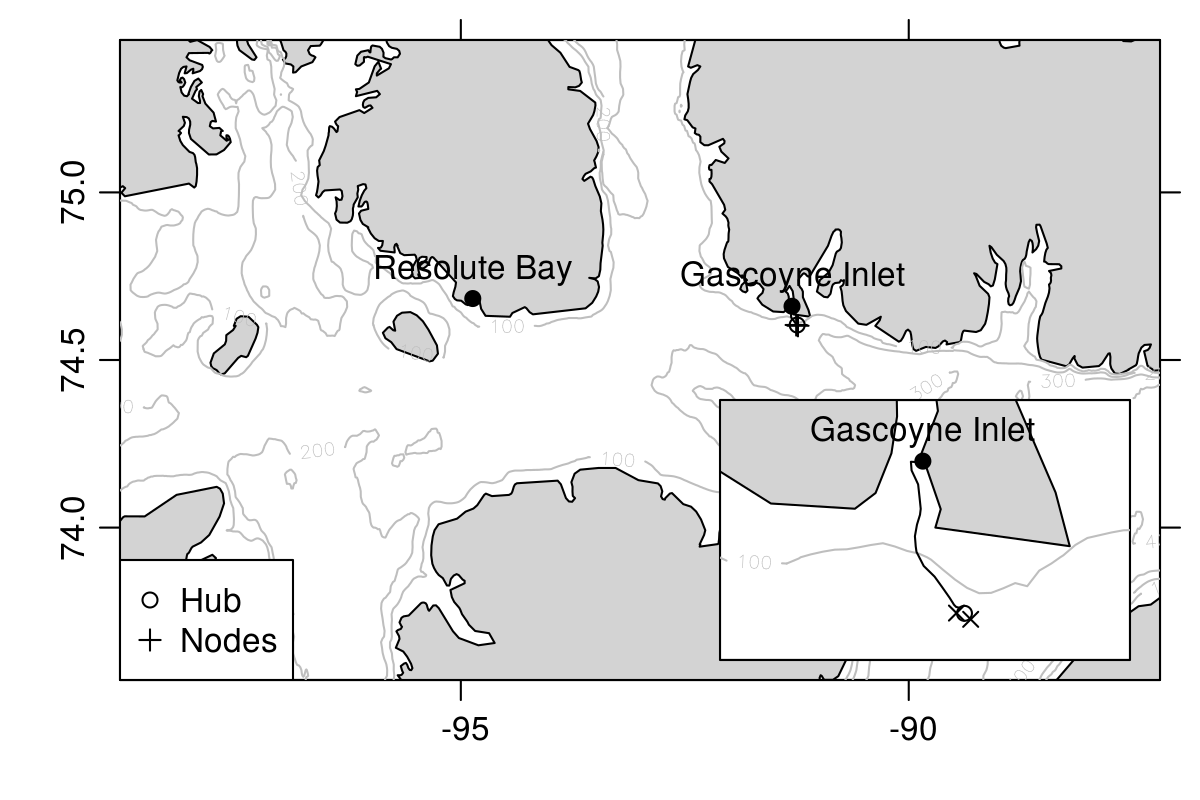
\includegraphics[width = 0.8\textwidth]{./figures/01_BSFieldSiteOverview.png}
\caption[Map of field site]{Map of the Barrow Strait field site showing the locations of the BSRTO Hub and Node moorings.}
\label{f:map}
\end{figure}



\begin{figure}
\centering
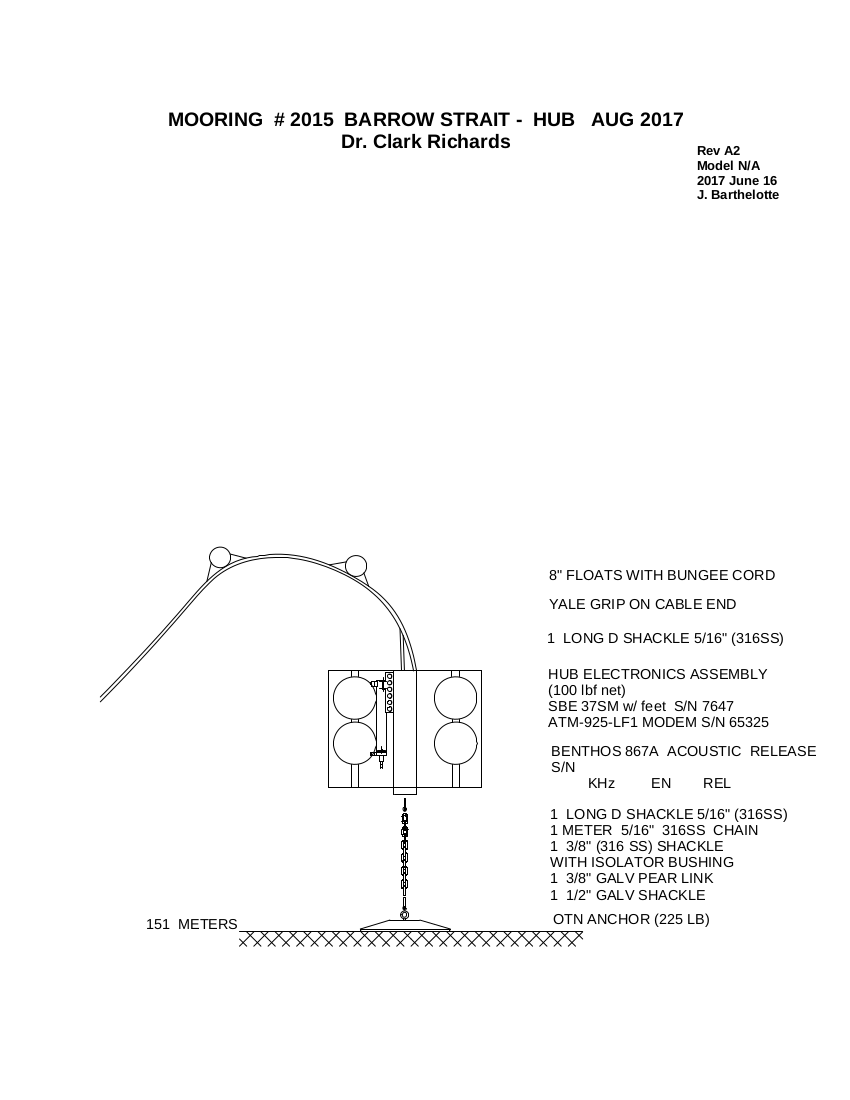
\includegraphics[width = 0.8\textwidth]{./figures/HUB.png}
\caption[Mooring Diagram: Hub]{Diagram of the Hub mooring.}
\label{f:md_hub}
\end{figure}

\begin{figure}
\centering
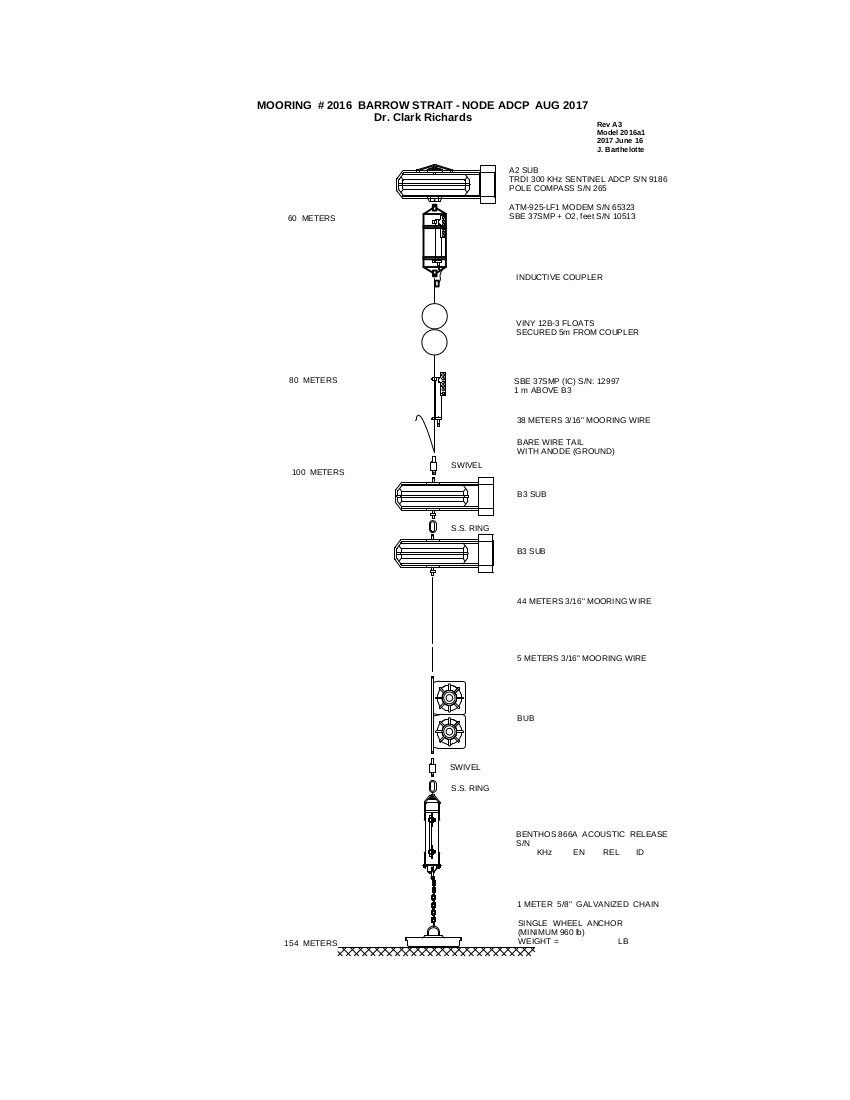
\includegraphics[width = 0.8\textwidth]{./figures/ADCP.png}
\caption[Mooring Diagram: ADCP Node]{Diagram of the ADCP Node mooring.}
\label{f:md_adcp}
\end{figure}

\begin{figure}
\centering
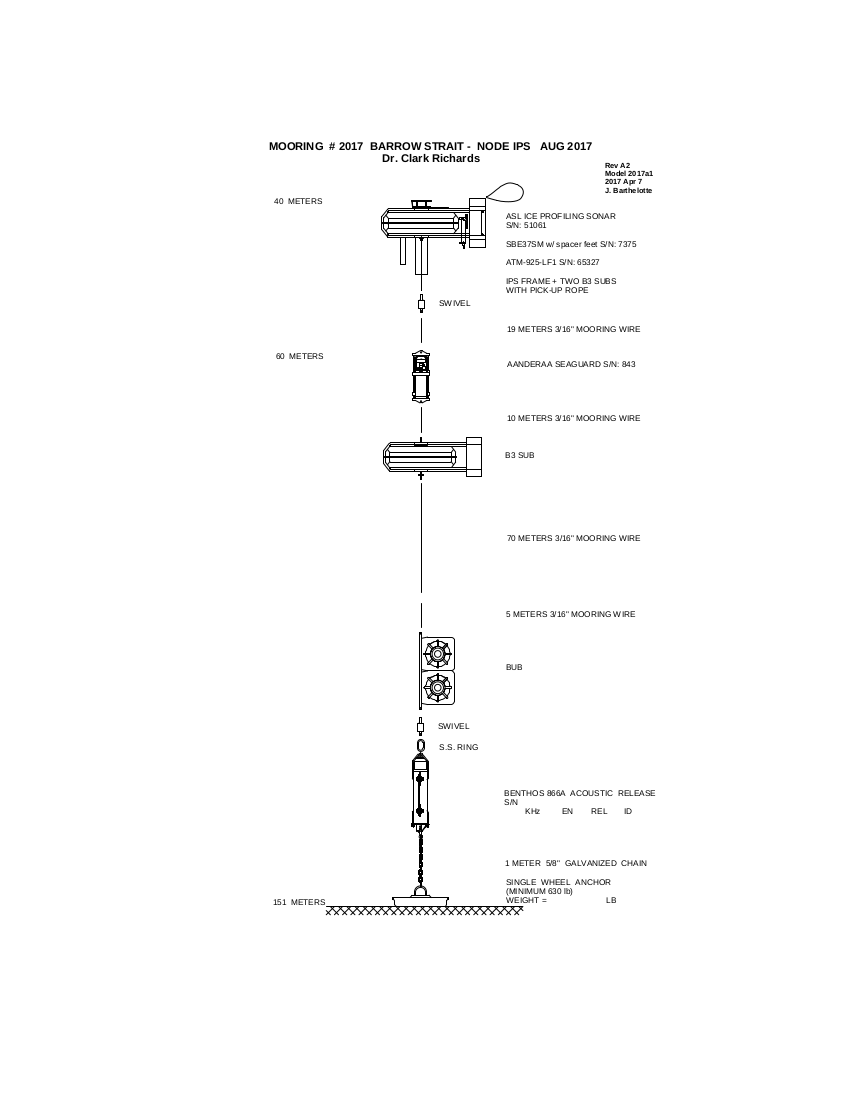
\includegraphics[width = 0.8\textwidth]{./figures/IPS.png}
\caption[Mooring Diagram: IPS node]{Diagram of the IPS Node mooring.}
\label{f:md_ips}
\end{figure}



\begin{figure}
\centering
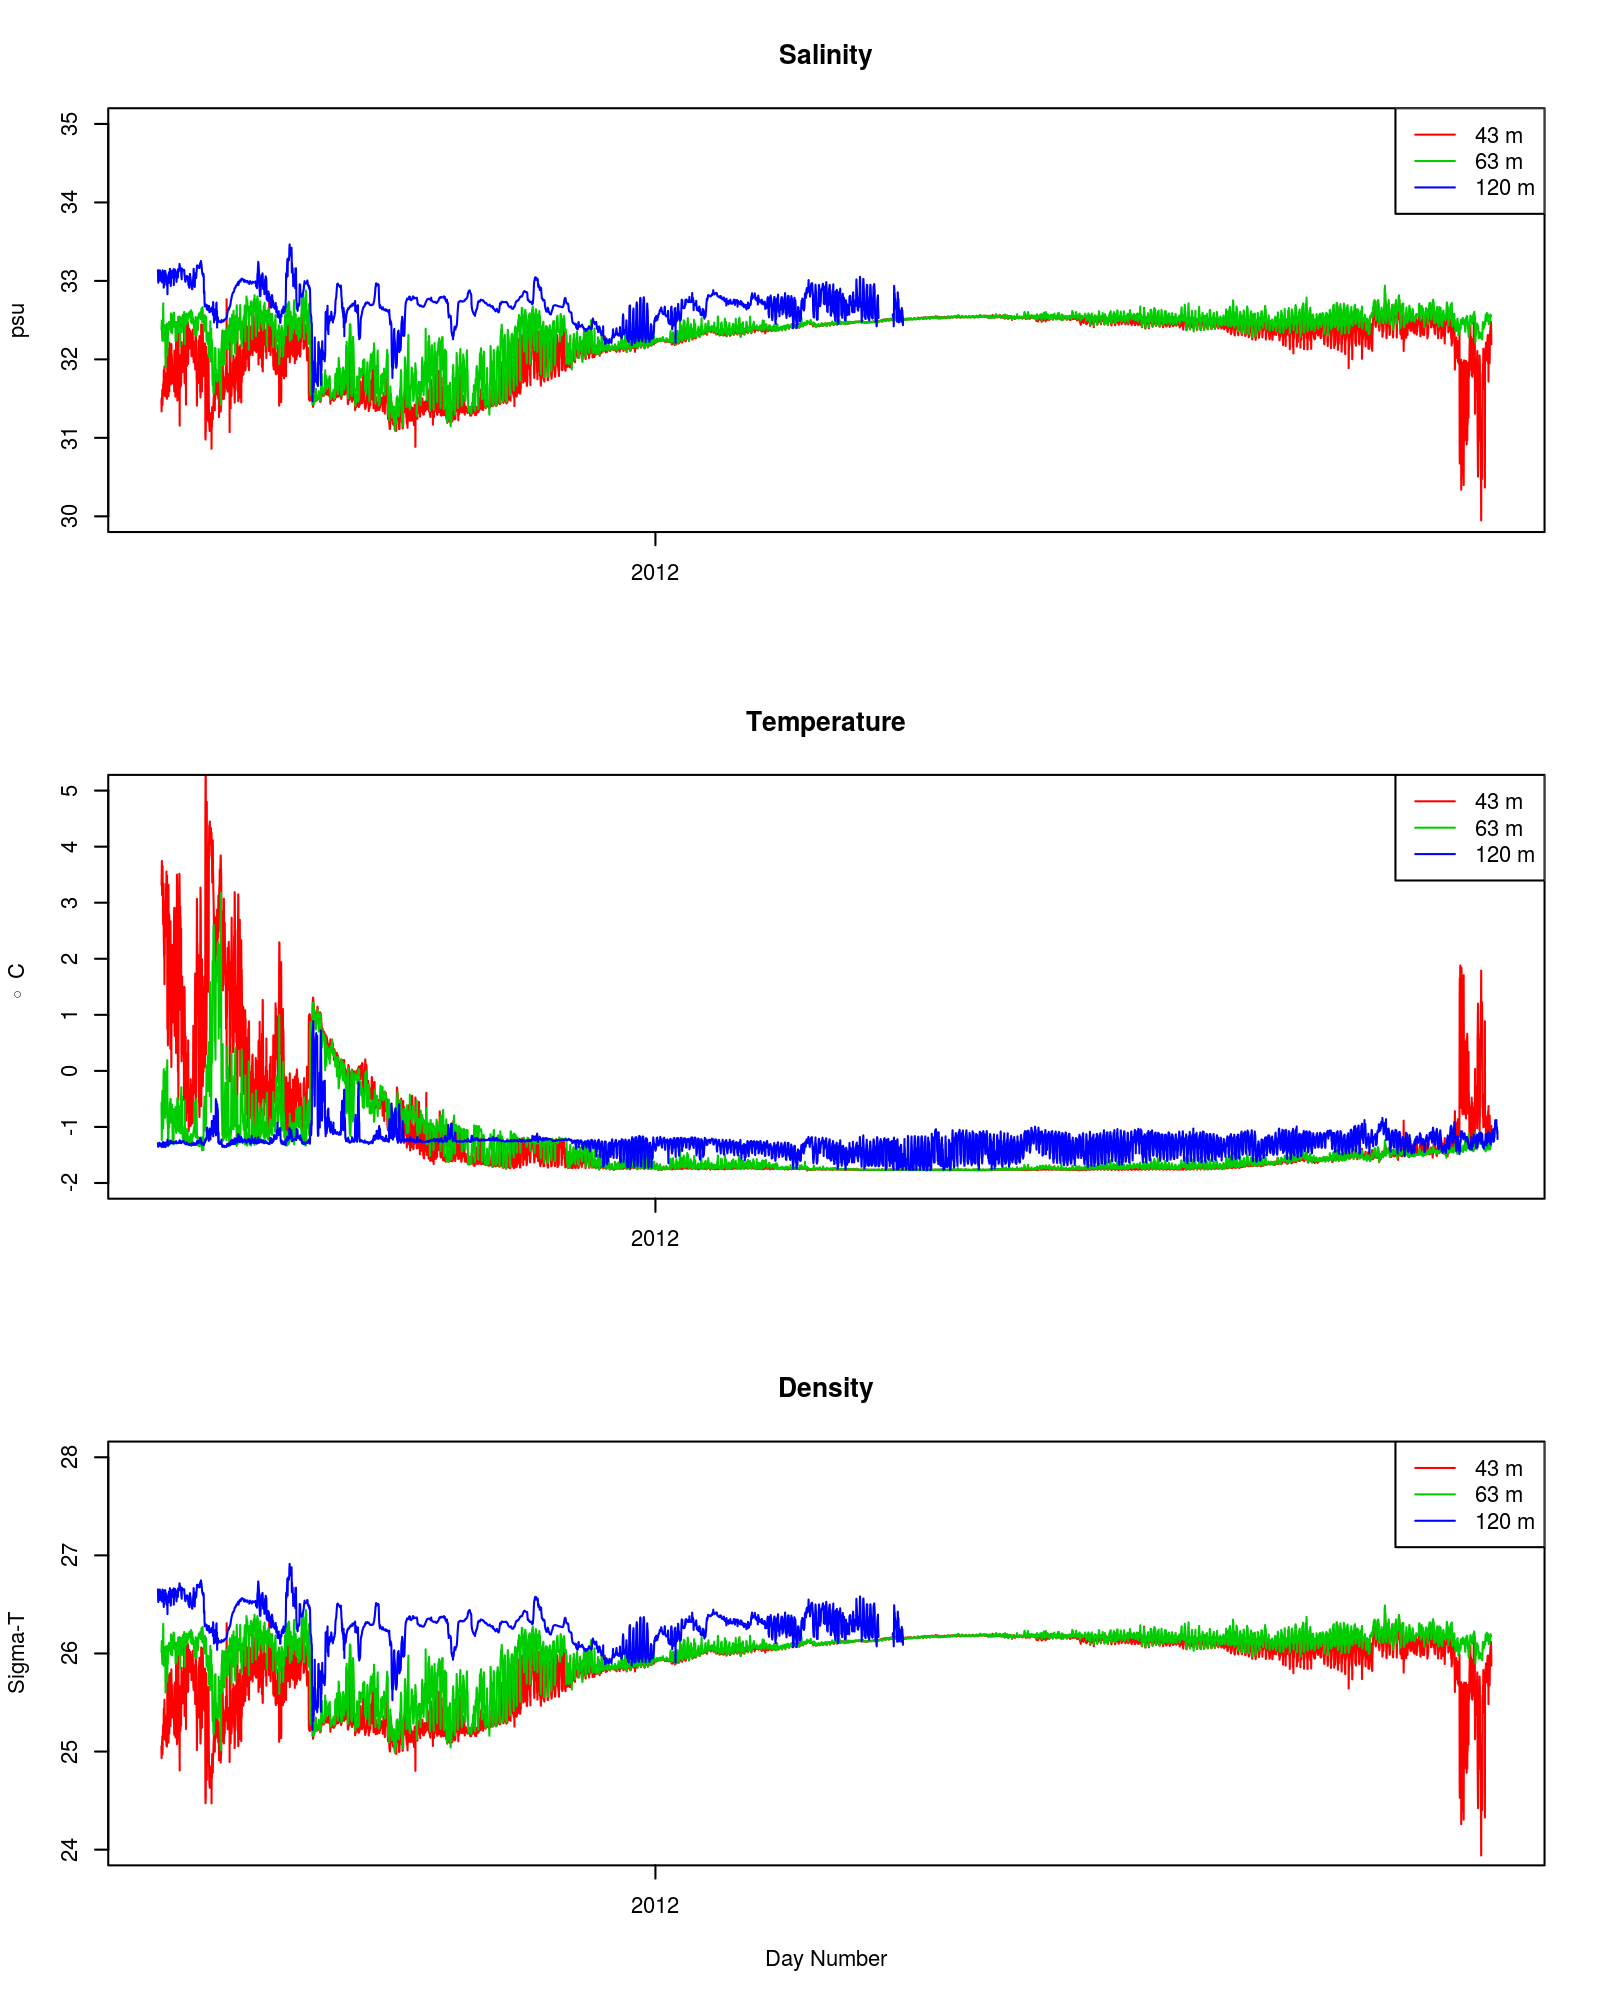
\includegraphics[width = 0.8\textwidth]{./figures/05_mctd_2011_2012.png}
\caption[Moored CTD, August 2011-2012]{Moored CTD data, August 2011 - August 2012.}
\label{f:mctd_2011_2012}
\end{figure}

\begin{figure}
\centering
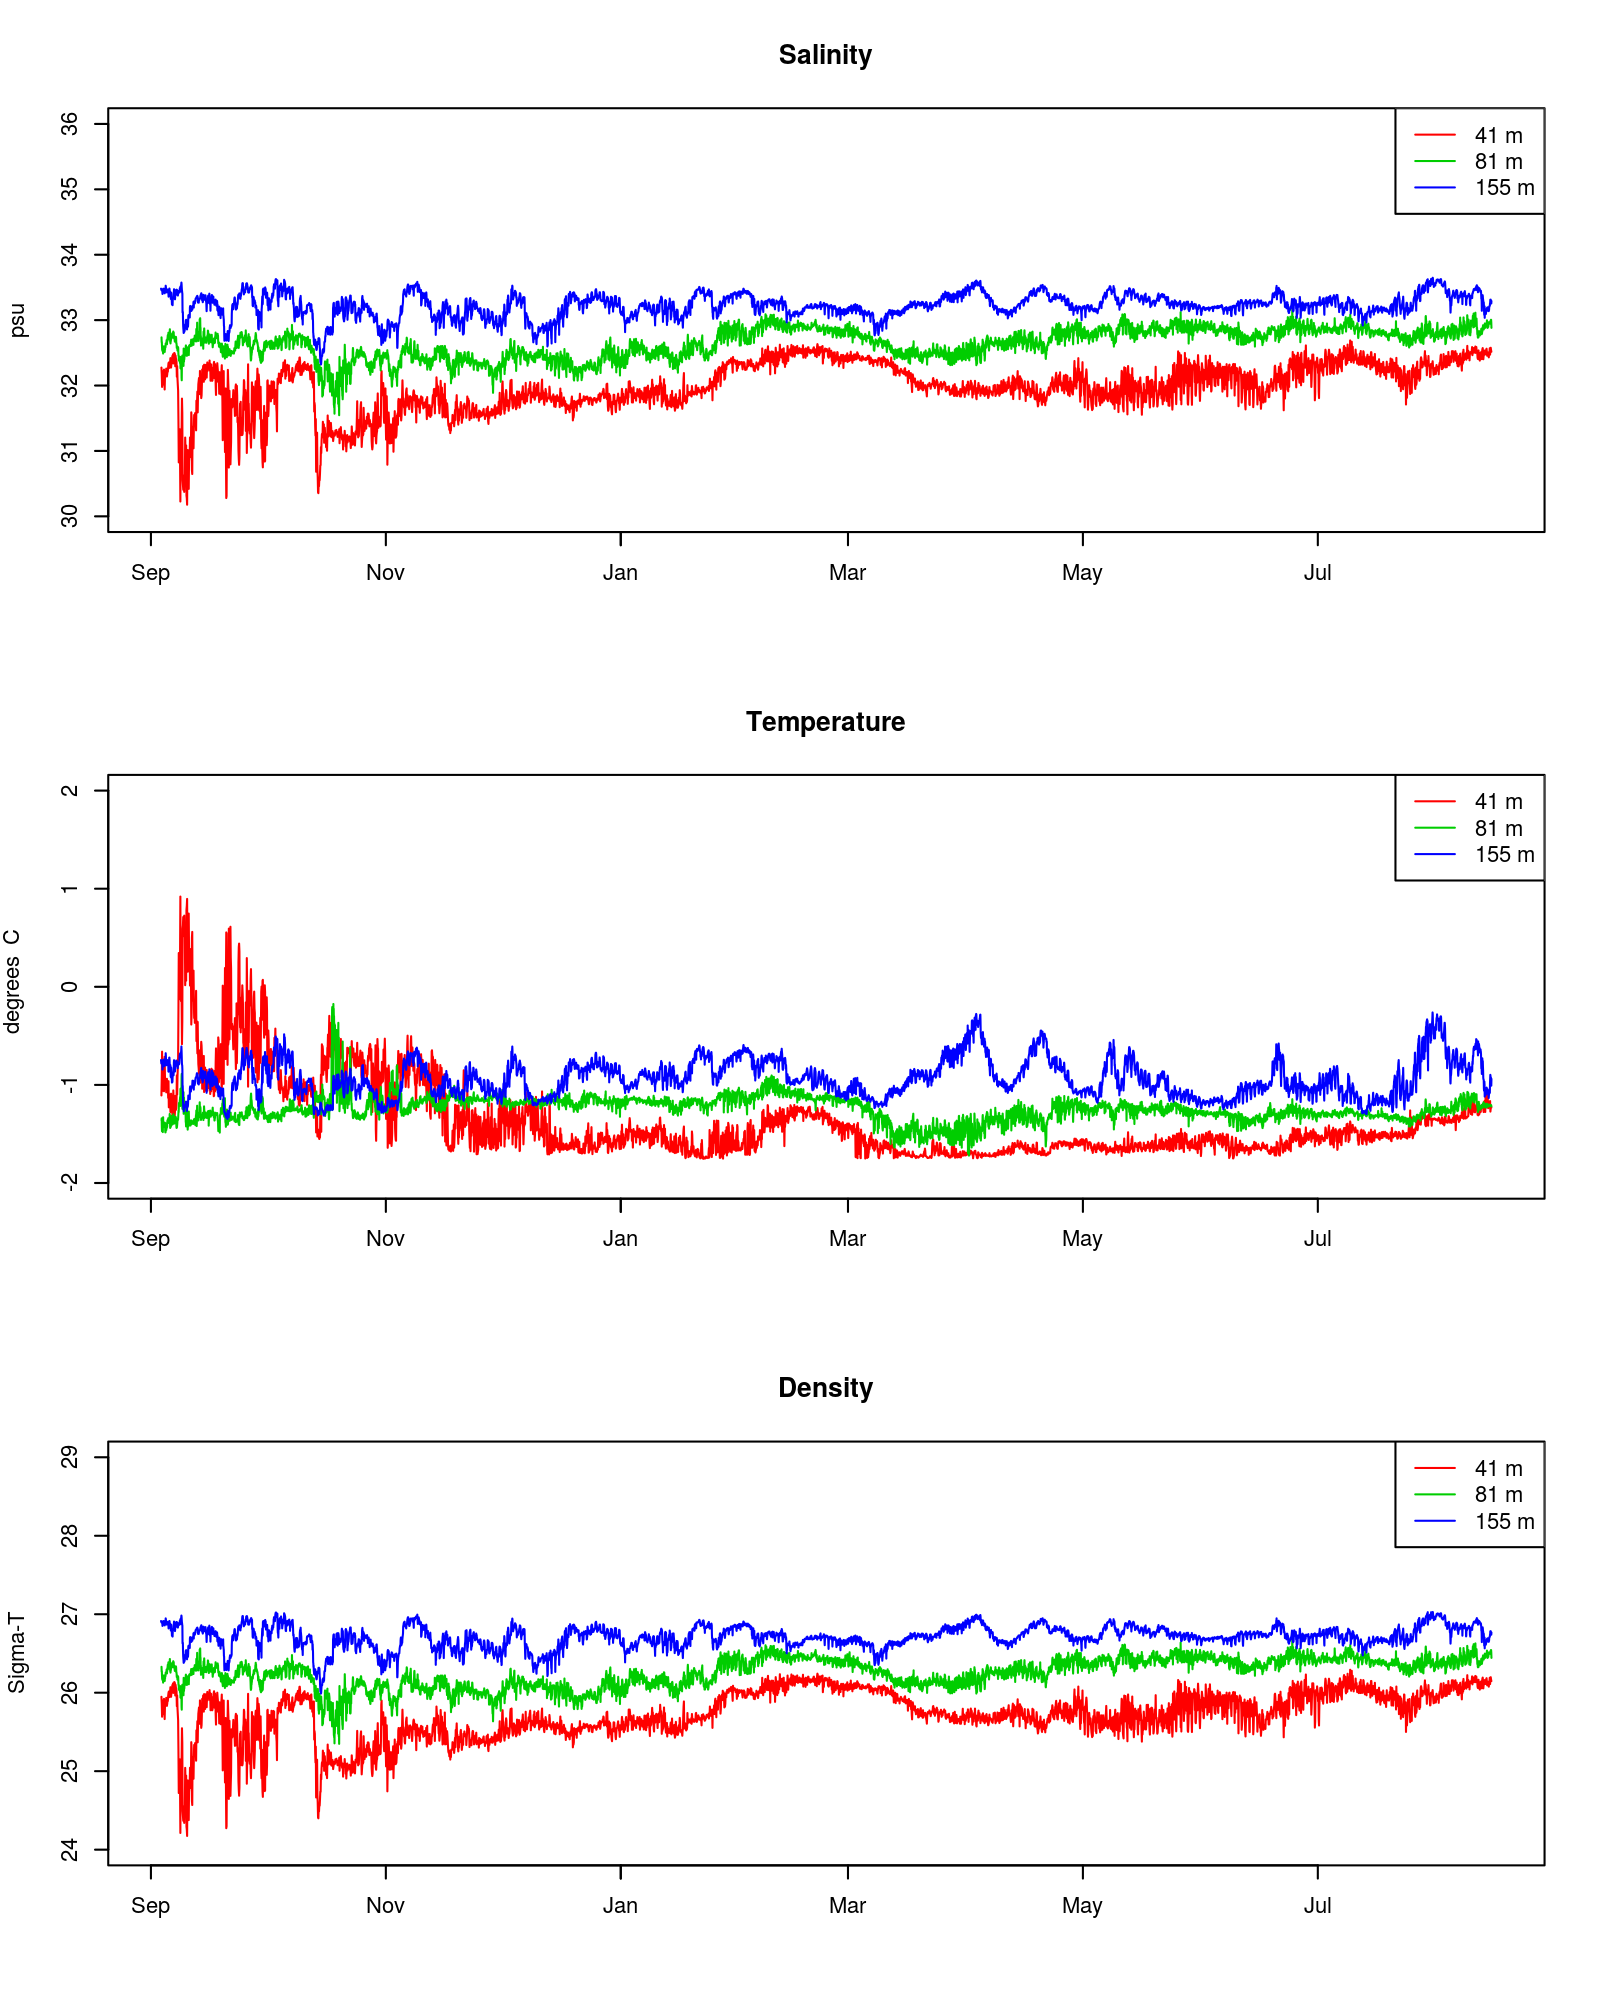
\includegraphics[width = 0.8\textwidth]{./figures/06_mctd_2012_2013.png}
\caption[Moored CTD, August 2012-2013]{Moored CTD data, August 2012 - August 2013.}
\label{f:mctd_2012_2013}
\end{figure}

\begin{figure}
\centering
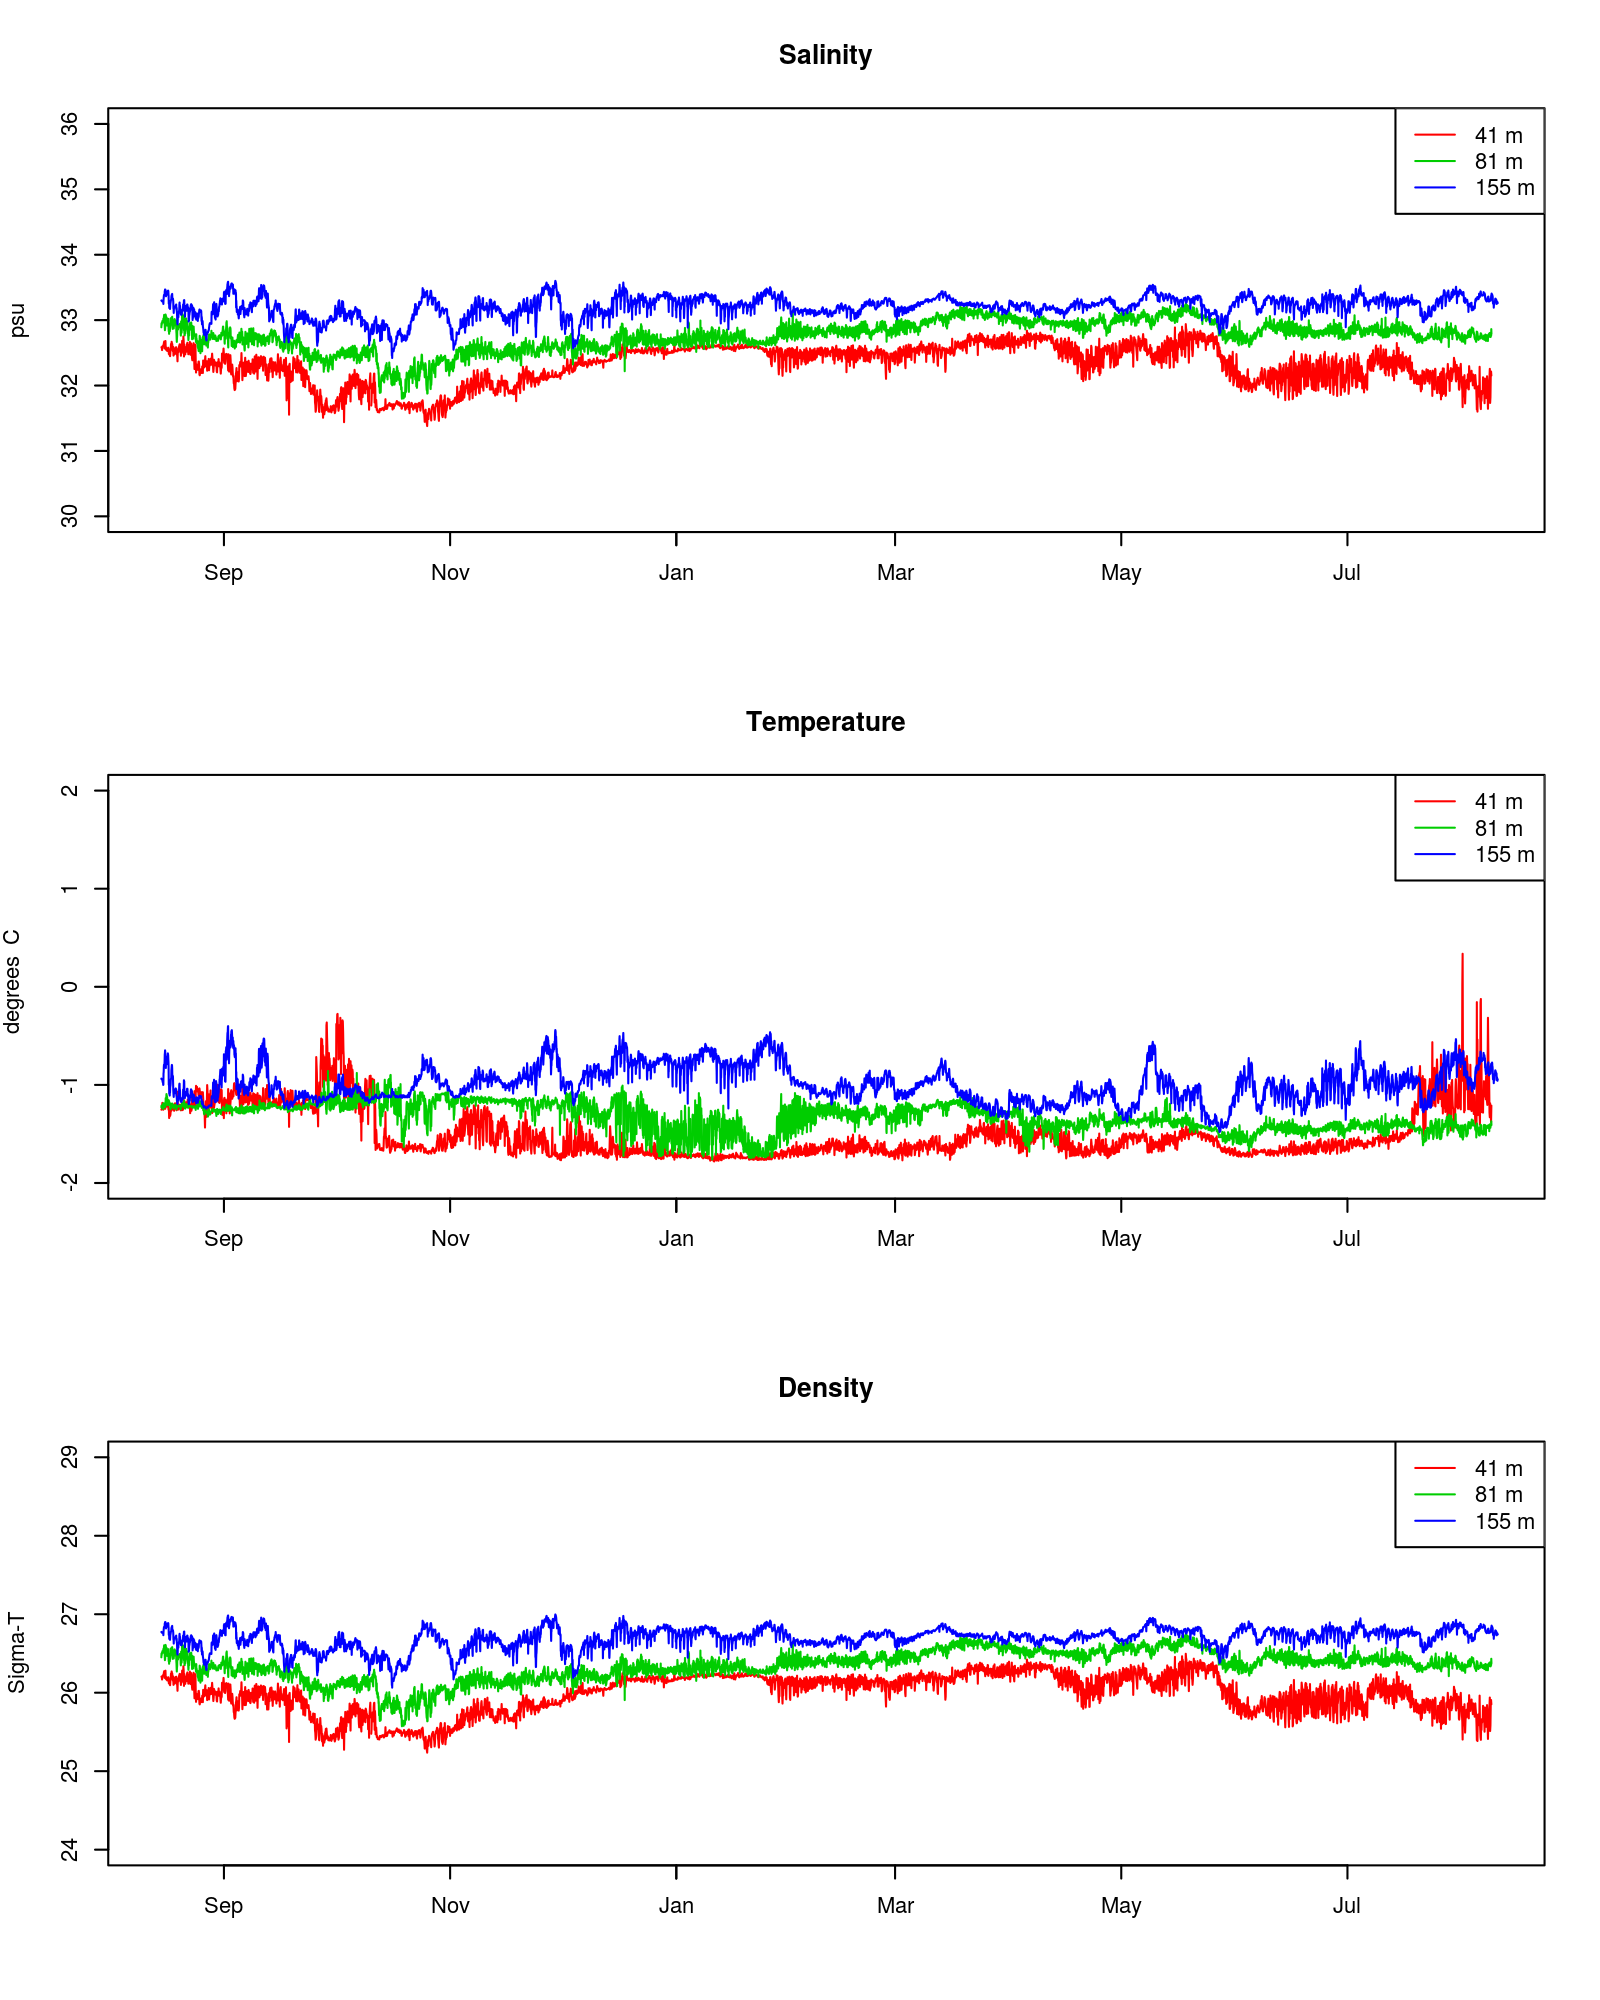
\includegraphics[width = 0.8\textwidth]{./figures/07_mctd_2013_2014.png}
\caption[Moored CTD, August 2013-2014]{Moored CTD data, August 2013 - August 2014.}
\label{f:mctd_2013_2014}
\end{figure}

\begin{figure}
\centering
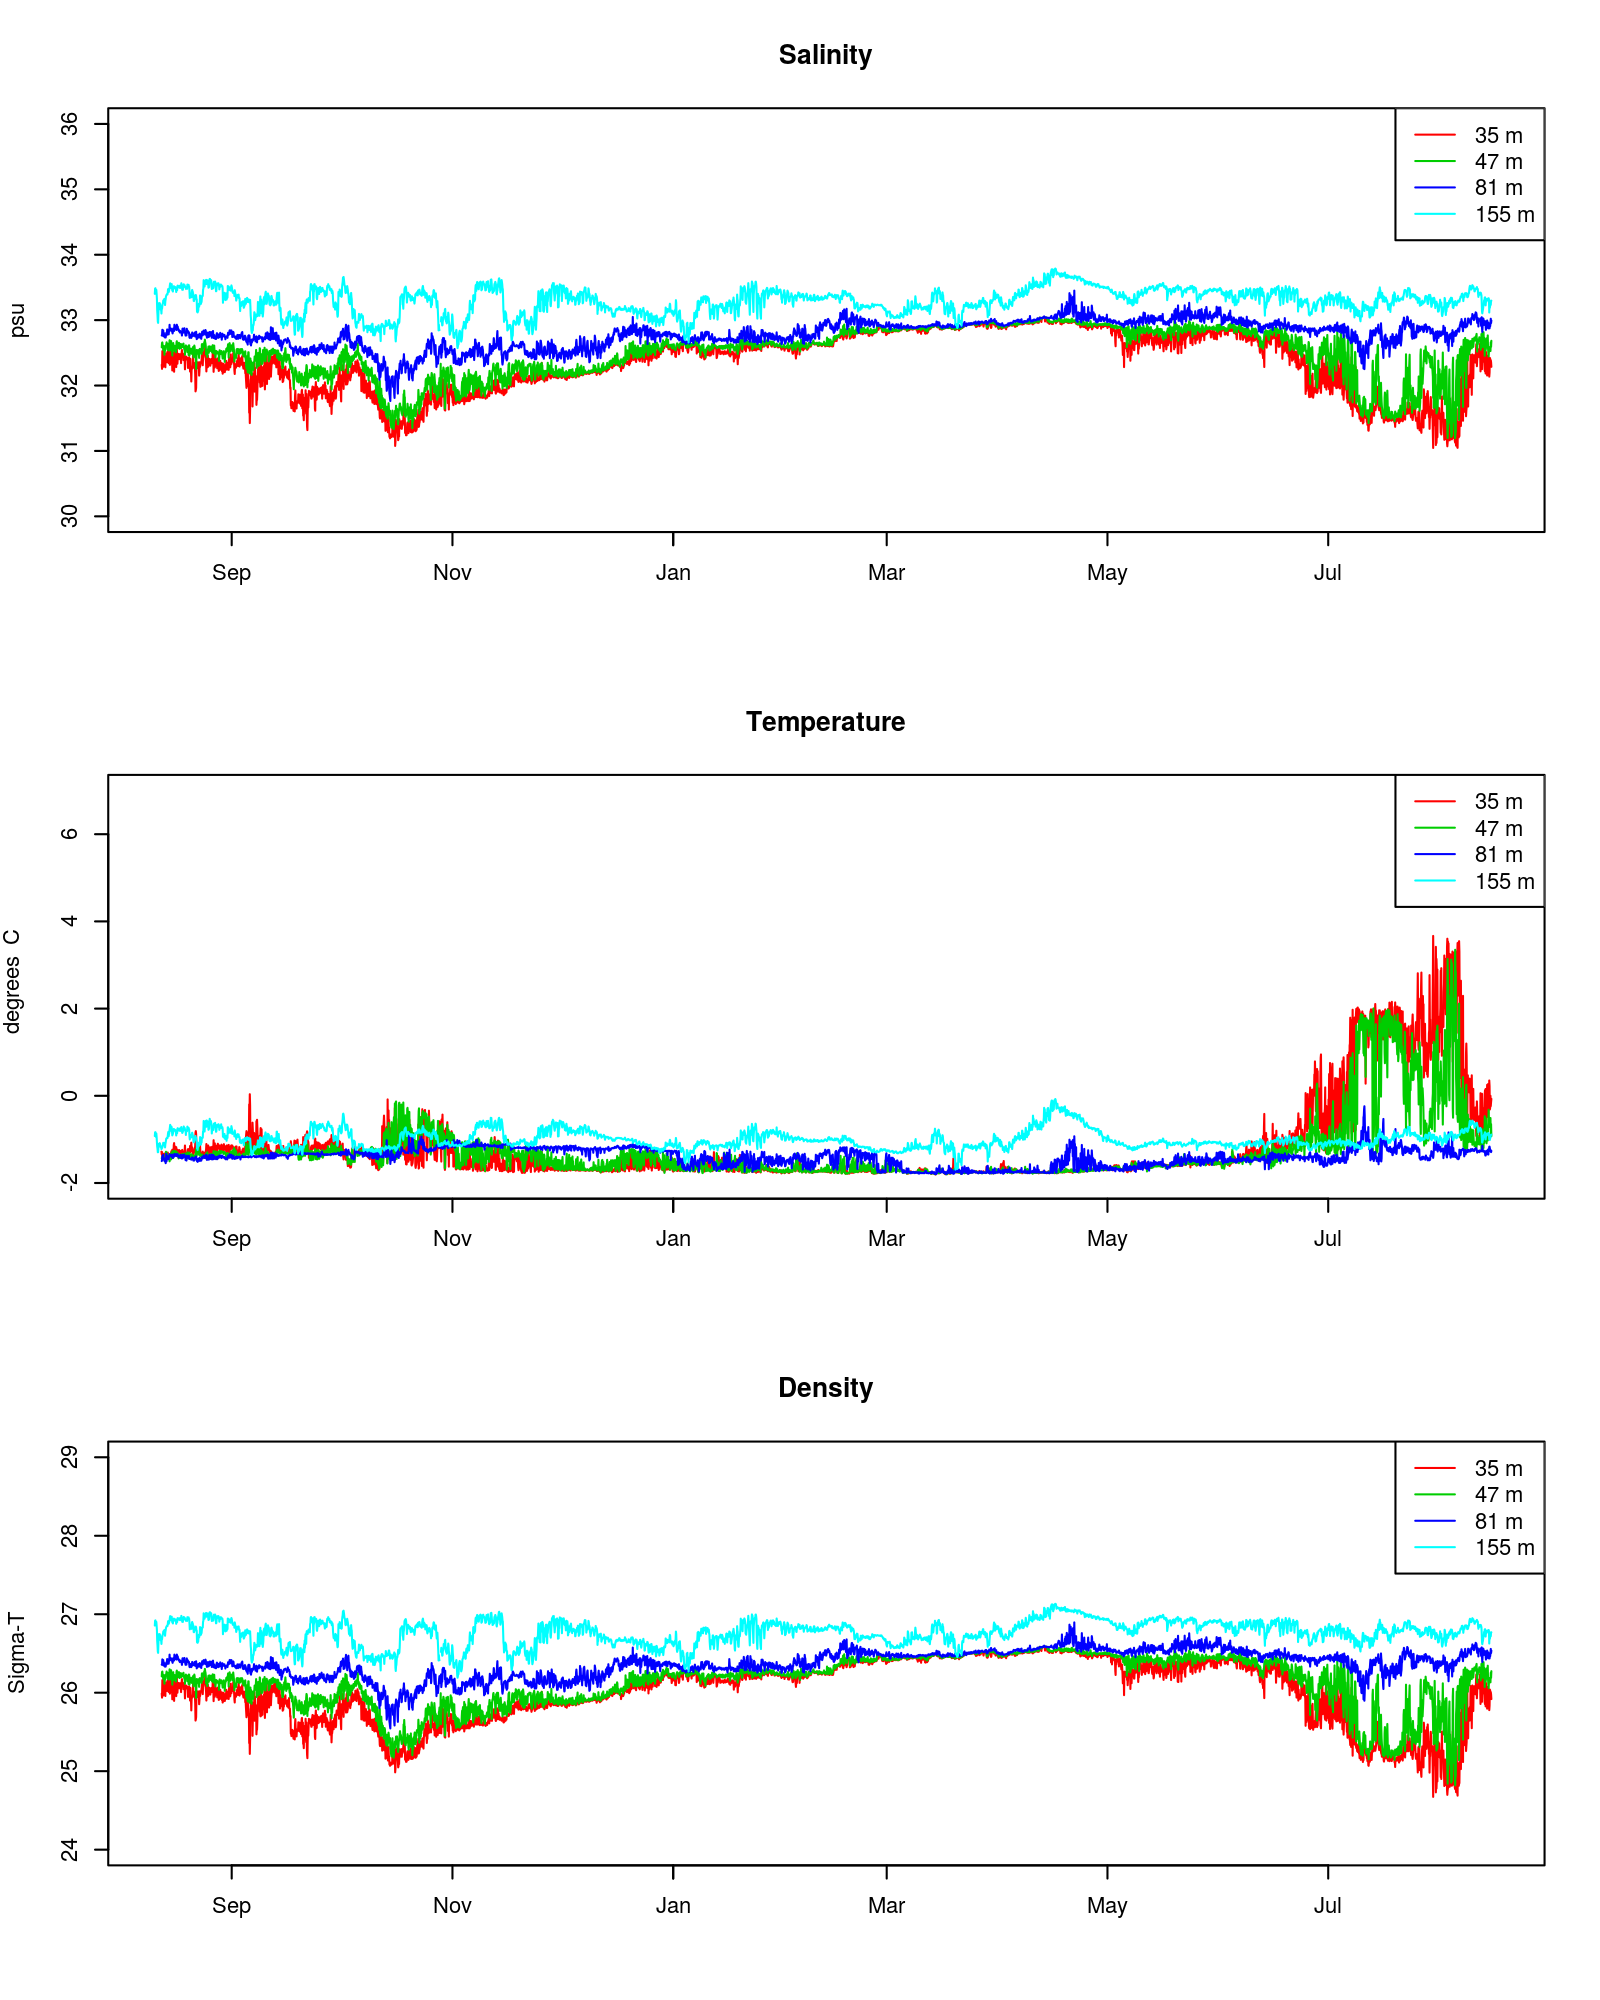
\includegraphics[width = 0.8\textwidth]{./figures/08_mctd_2014_2015.png}
\caption[Moored CTD, August 2014-2015]{Moored CTD data, August 2014 - August 2015.}
\label{f:mctd_2014_2015}
\end{figure}

\begin{figure}
\centering
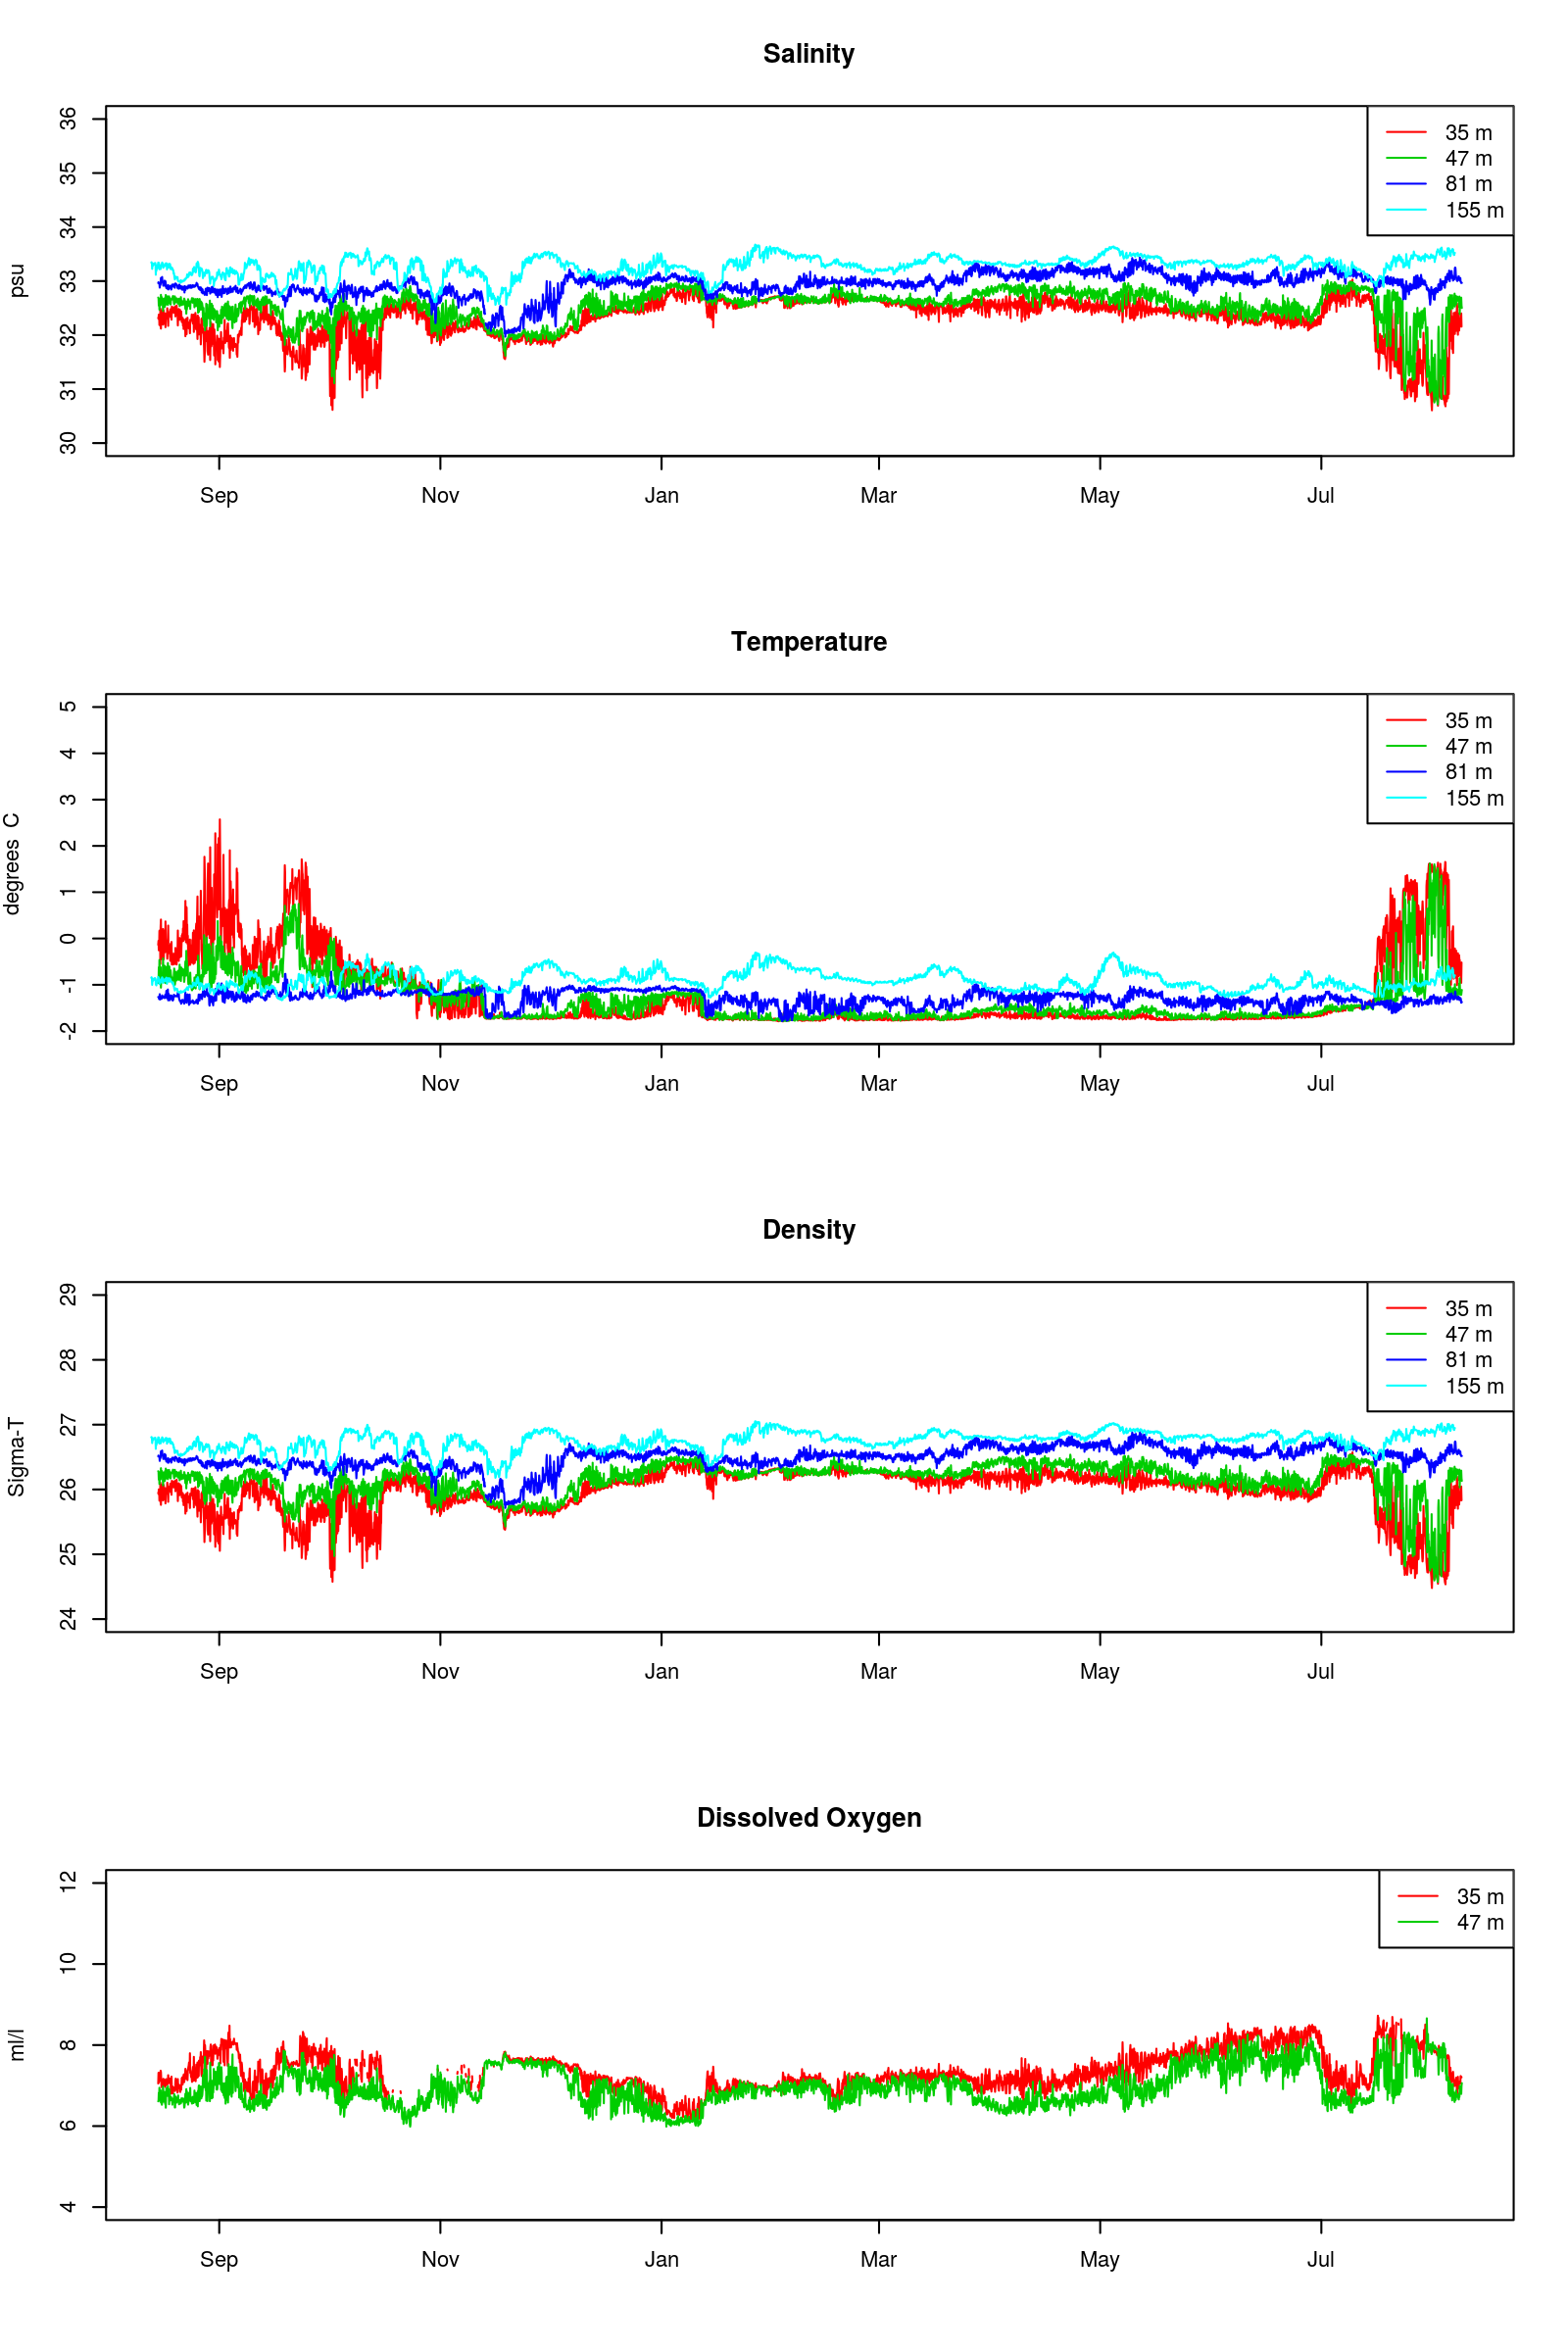
\includegraphics[width = 0.8\textwidth]{./figures/09_mctd_2015_2016.png}
\caption[Moored CTD, August 2015-2016]{Moored CTD data, August 2015 - August 2016.}
\label{f:mctd_2015_2016}
\end{figure}



\begin{figure}
\centering
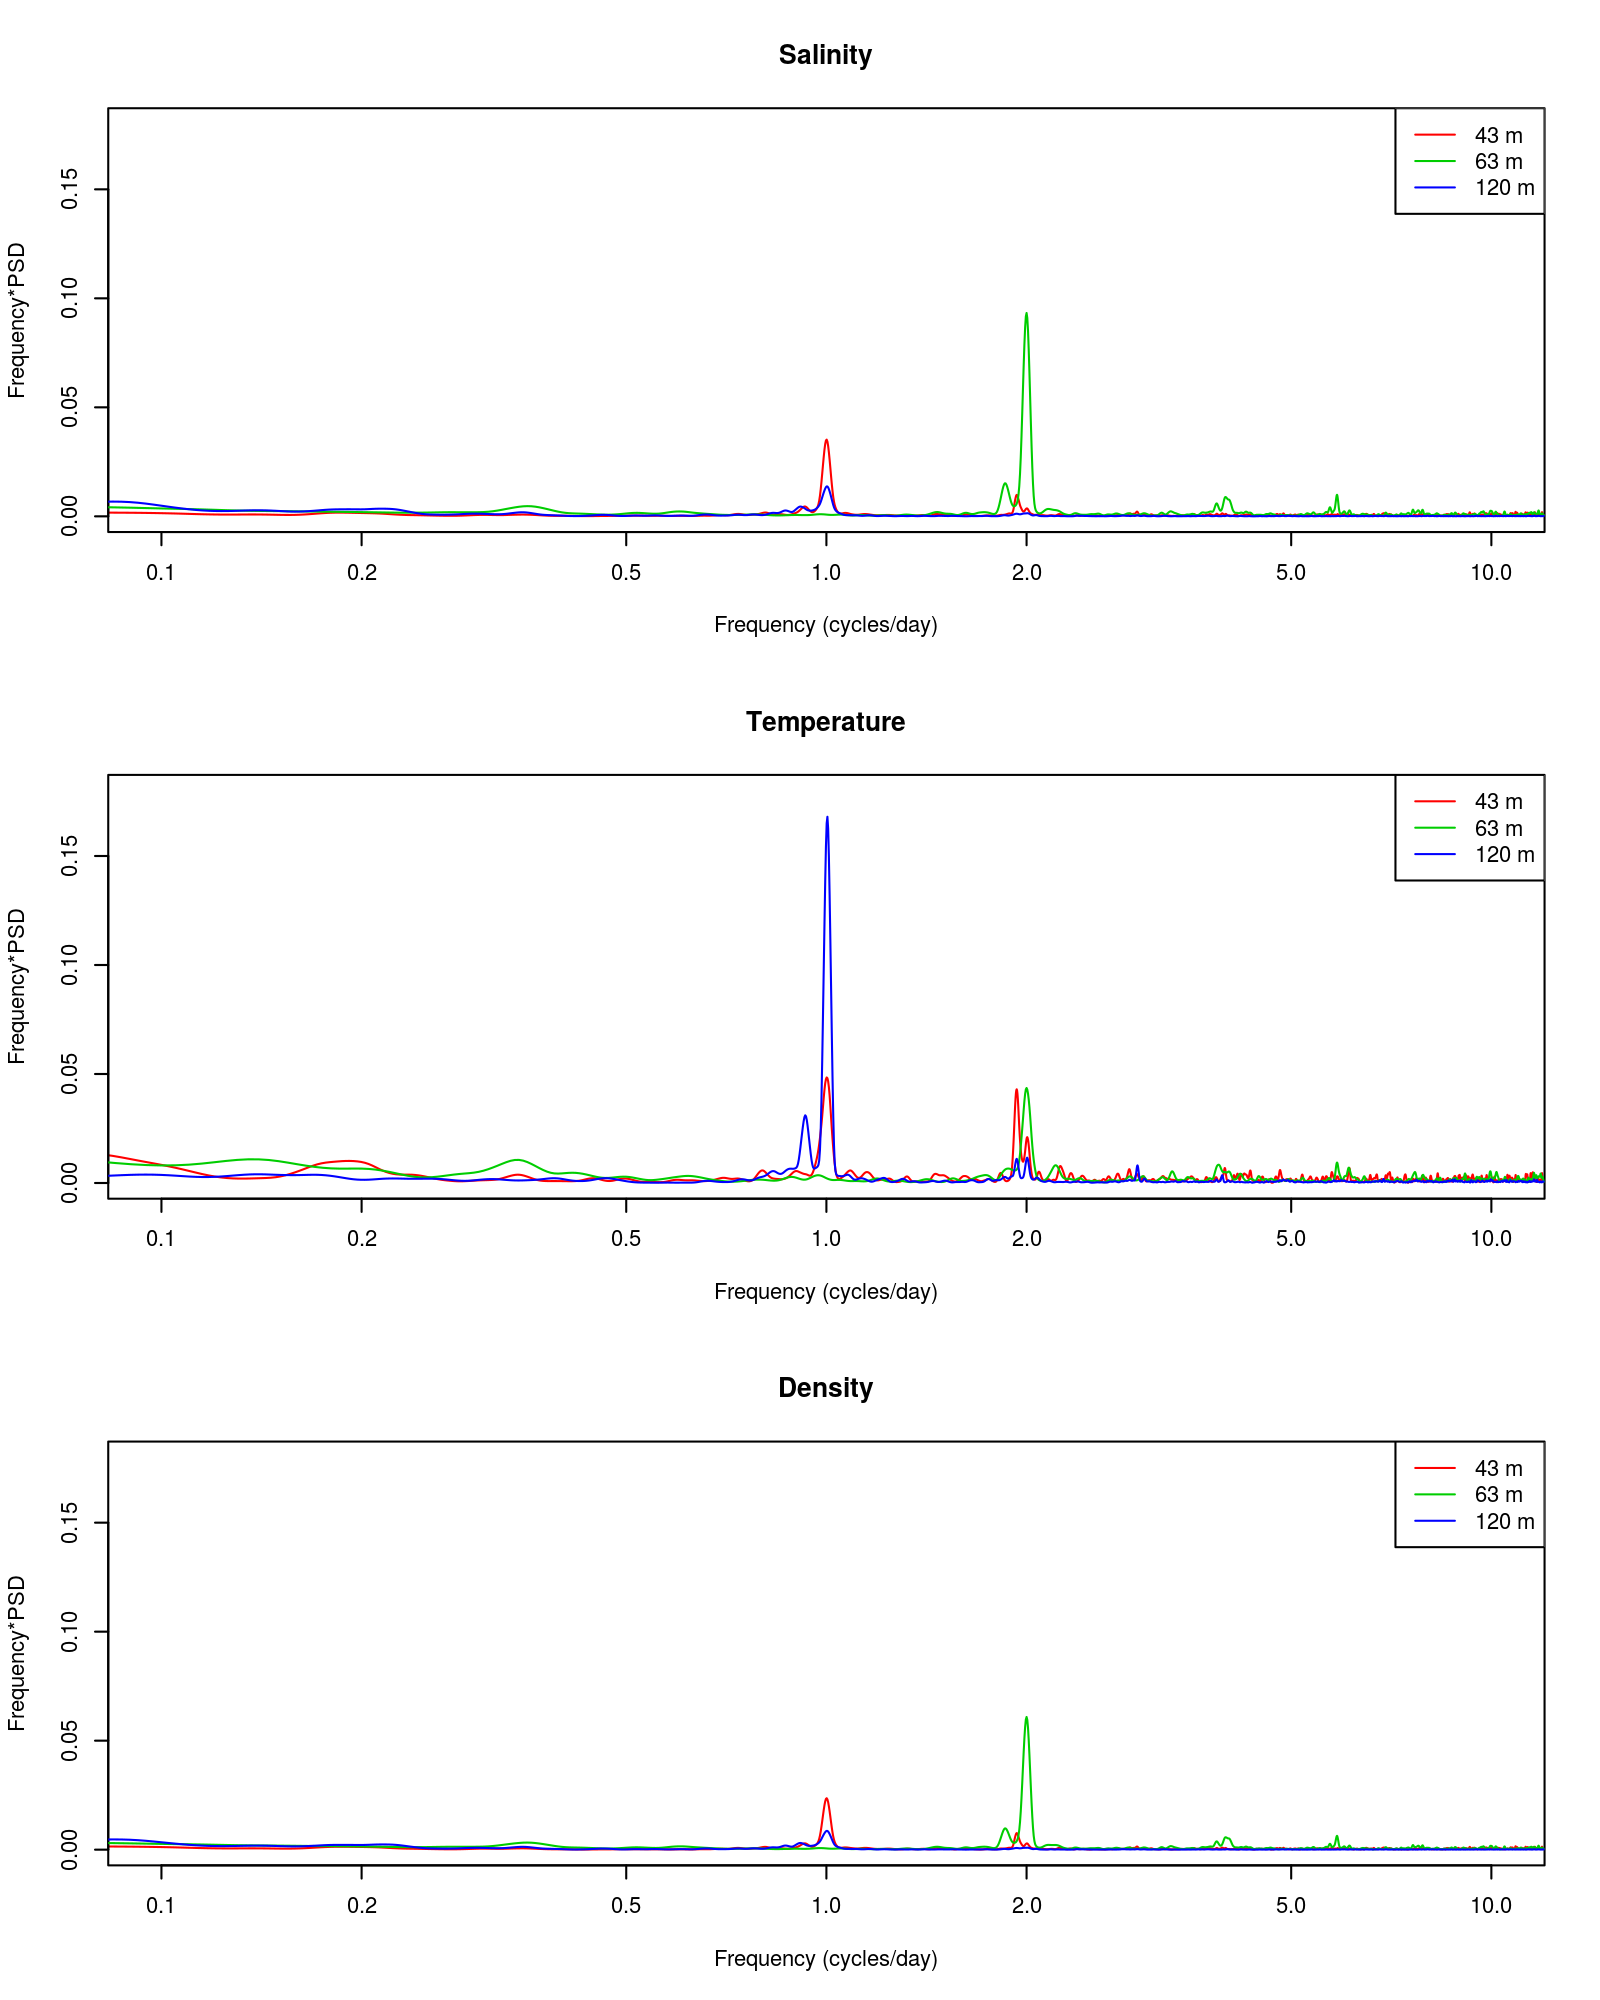
\includegraphics[width = 0.8\textwidth]{./figures/10_mctd_ps_2011_2012.png}
\caption[Power spectra of moored CTD, 2011-2012]{Power spectra of moored CTD data, August 2011 - August 2012.}
\label{f:mctd_ps_2011_2012}
\end{figure}

\begin{figure}
\centering
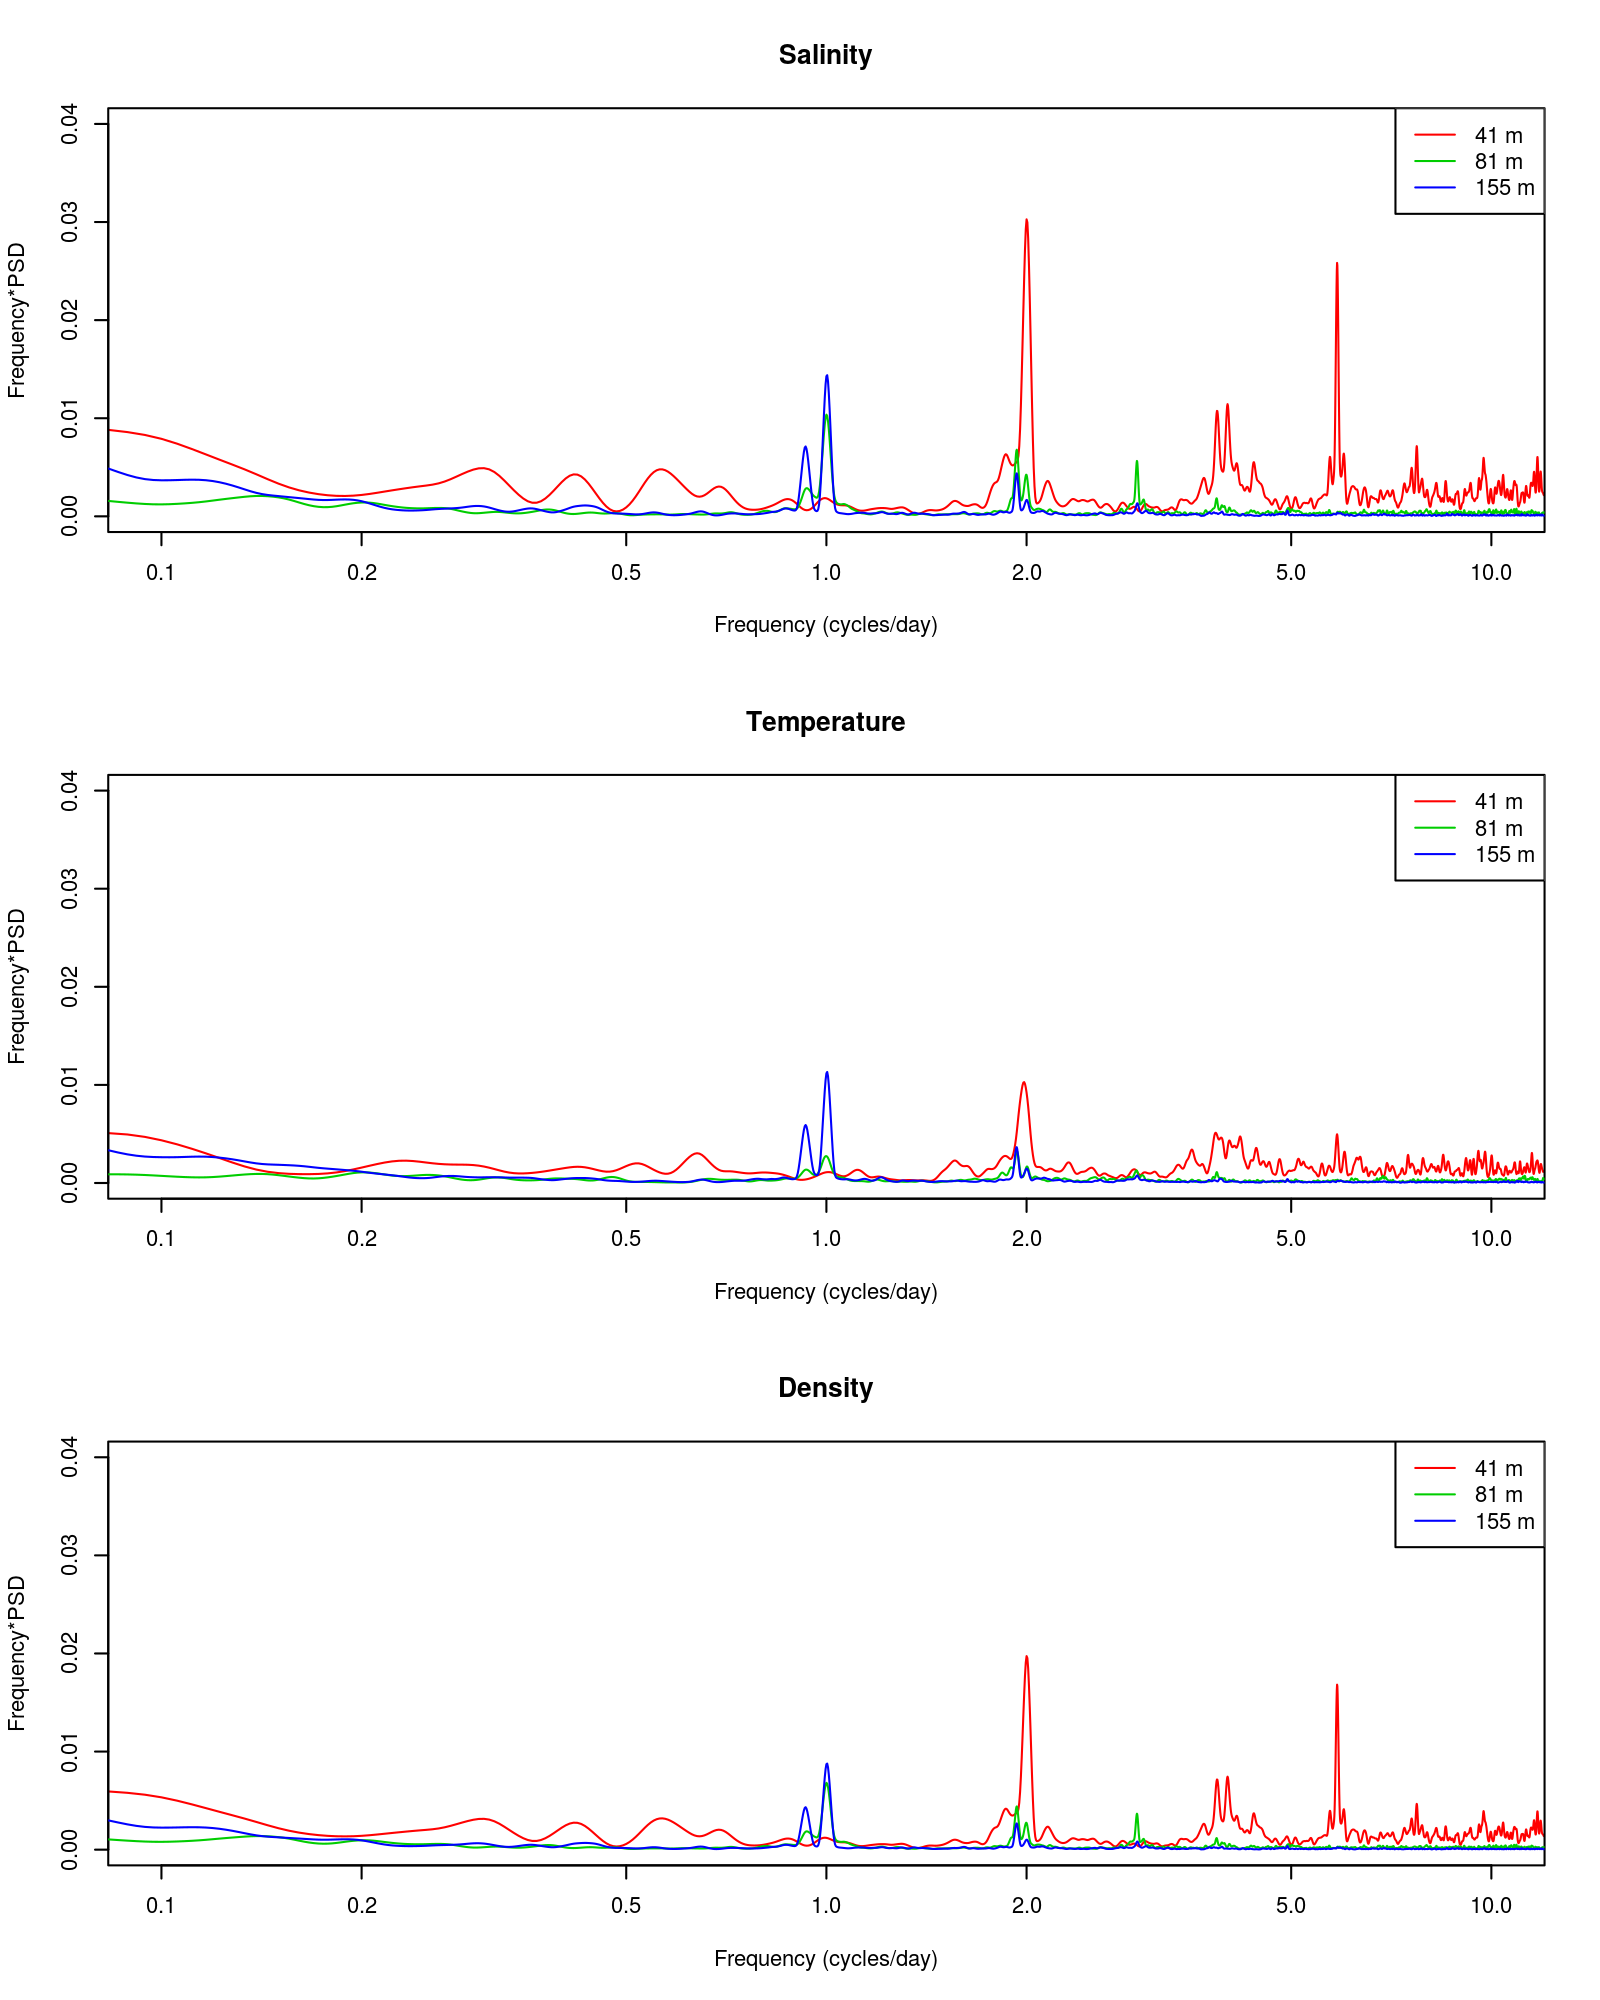
\includegraphics[width = 0.8\textwidth]{./figures/11_mctd_ps_2012_2013.png}
\caption[Power spectra of moored CTD, 2012-2013]{Power spectra of moored CTD data, August 2012 - August 2013.}
\label{f:mctd_ps_2012_2013}
\end{figure}

\begin{figure}
\centering
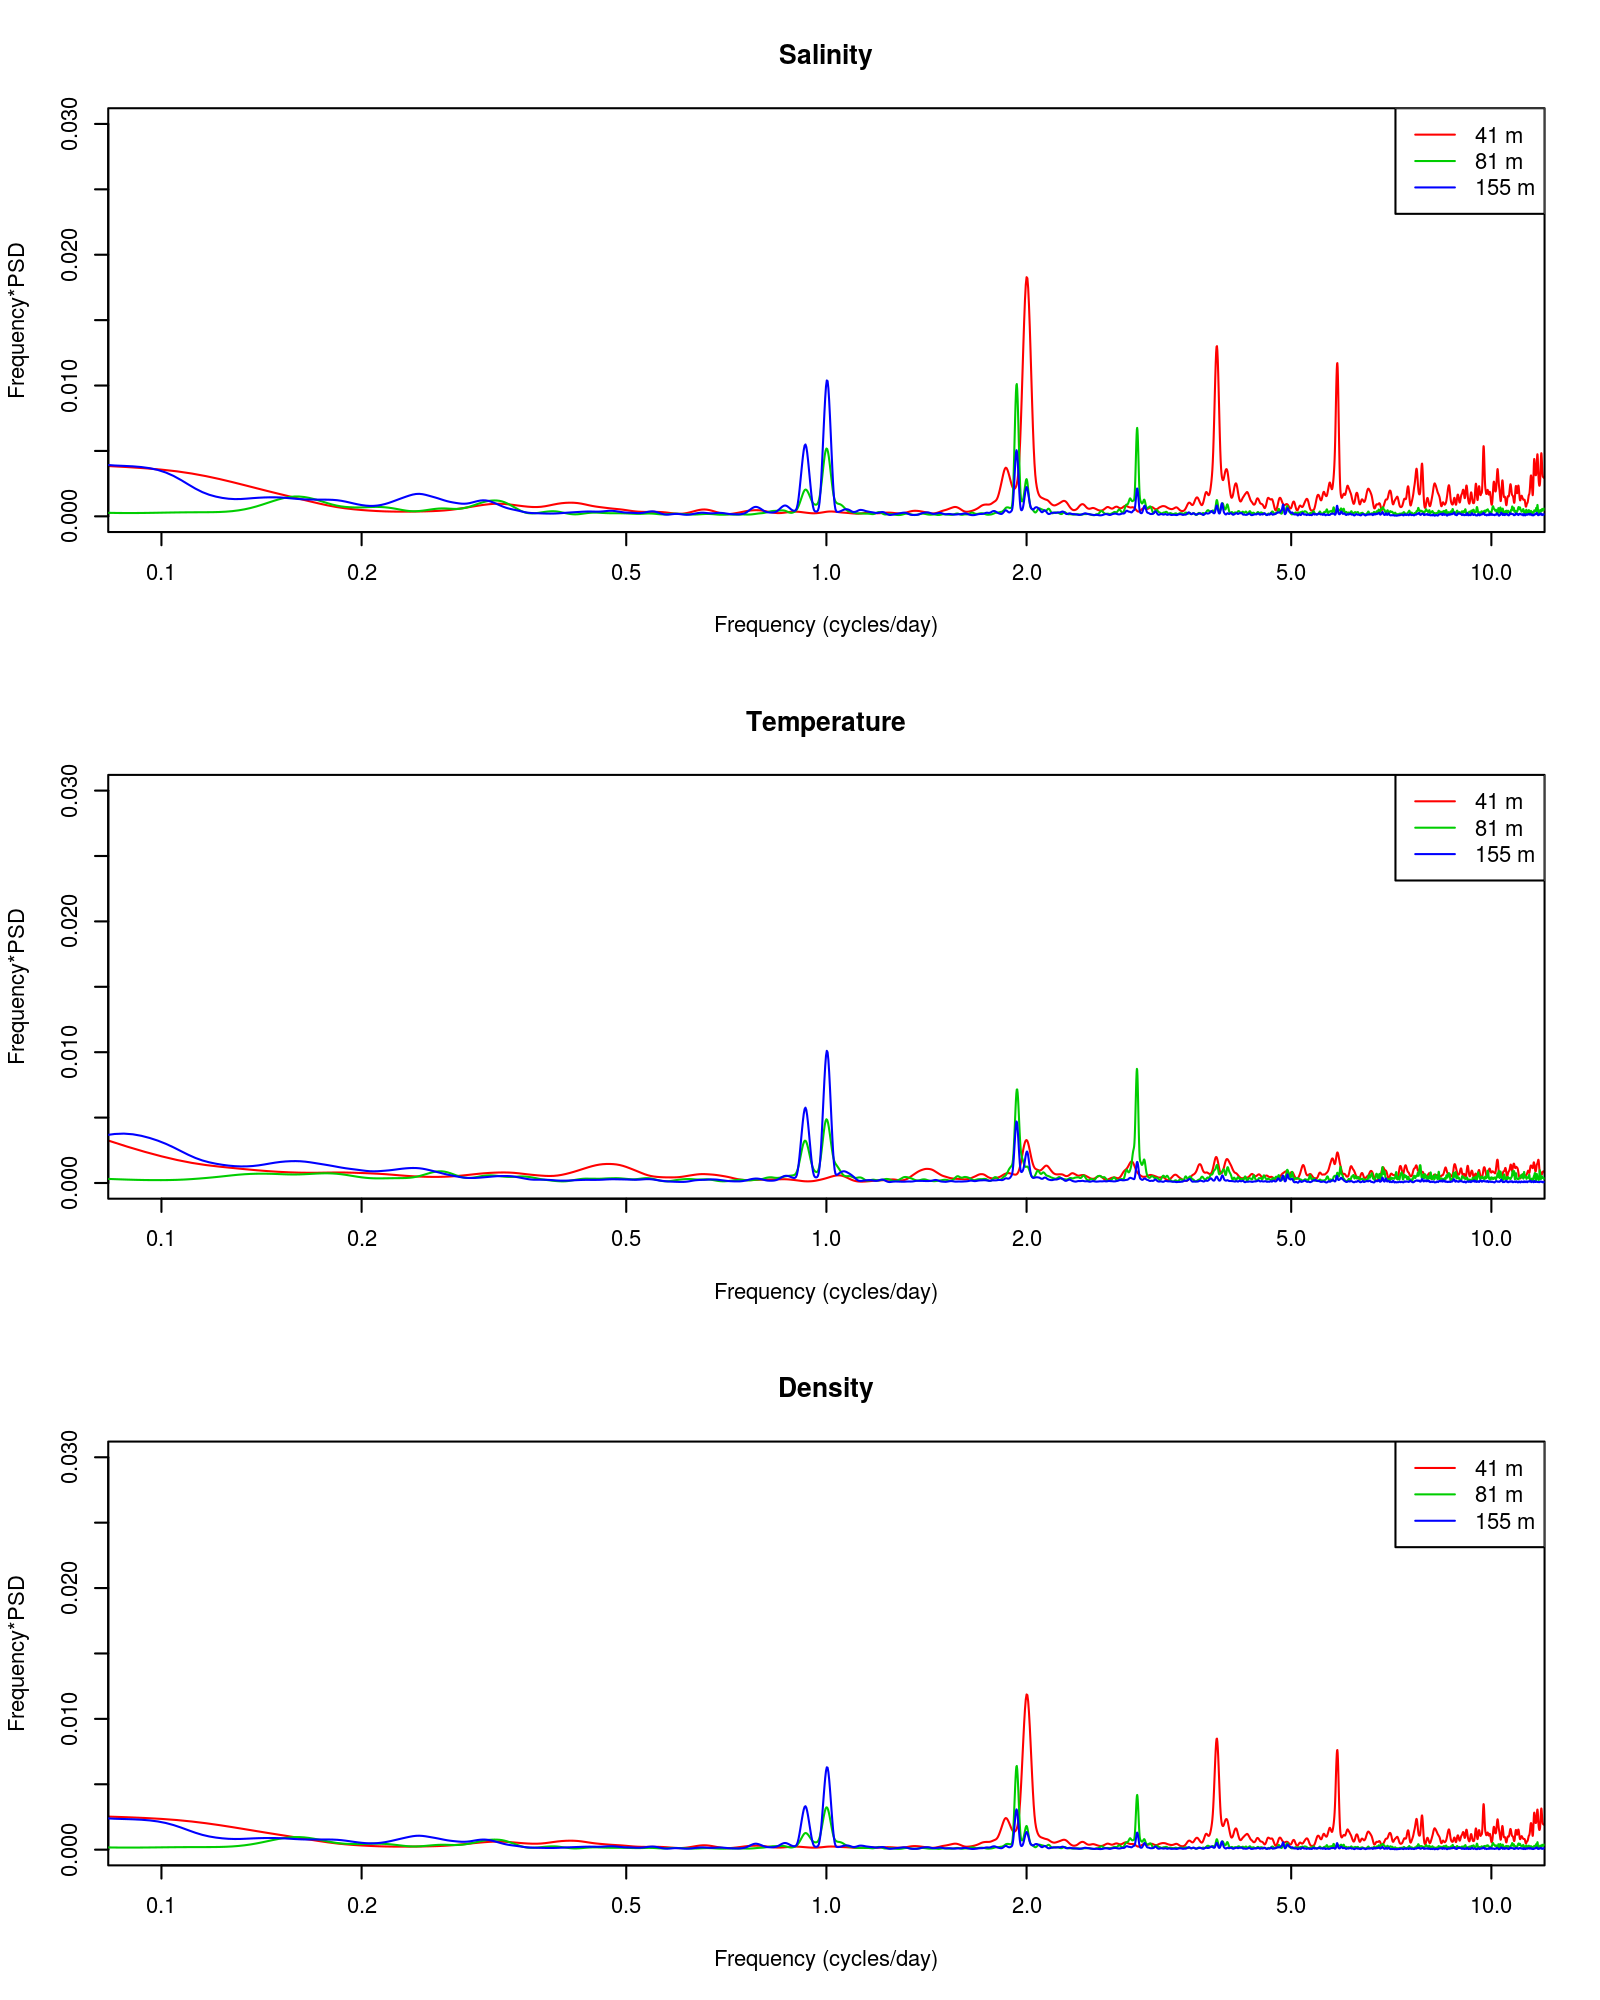
\includegraphics[width = 0.8\textwidth]{./figures/12_mctd_ps_2013_2014.png}
\caption[Power spectra of moored CTD, 2013-2014]{Power spectra of moored CTD data, August 2013 - August 2014.}
\label{f:mctd_ps_2013_2014}
\end{figure}

\begin{figure}
\centering
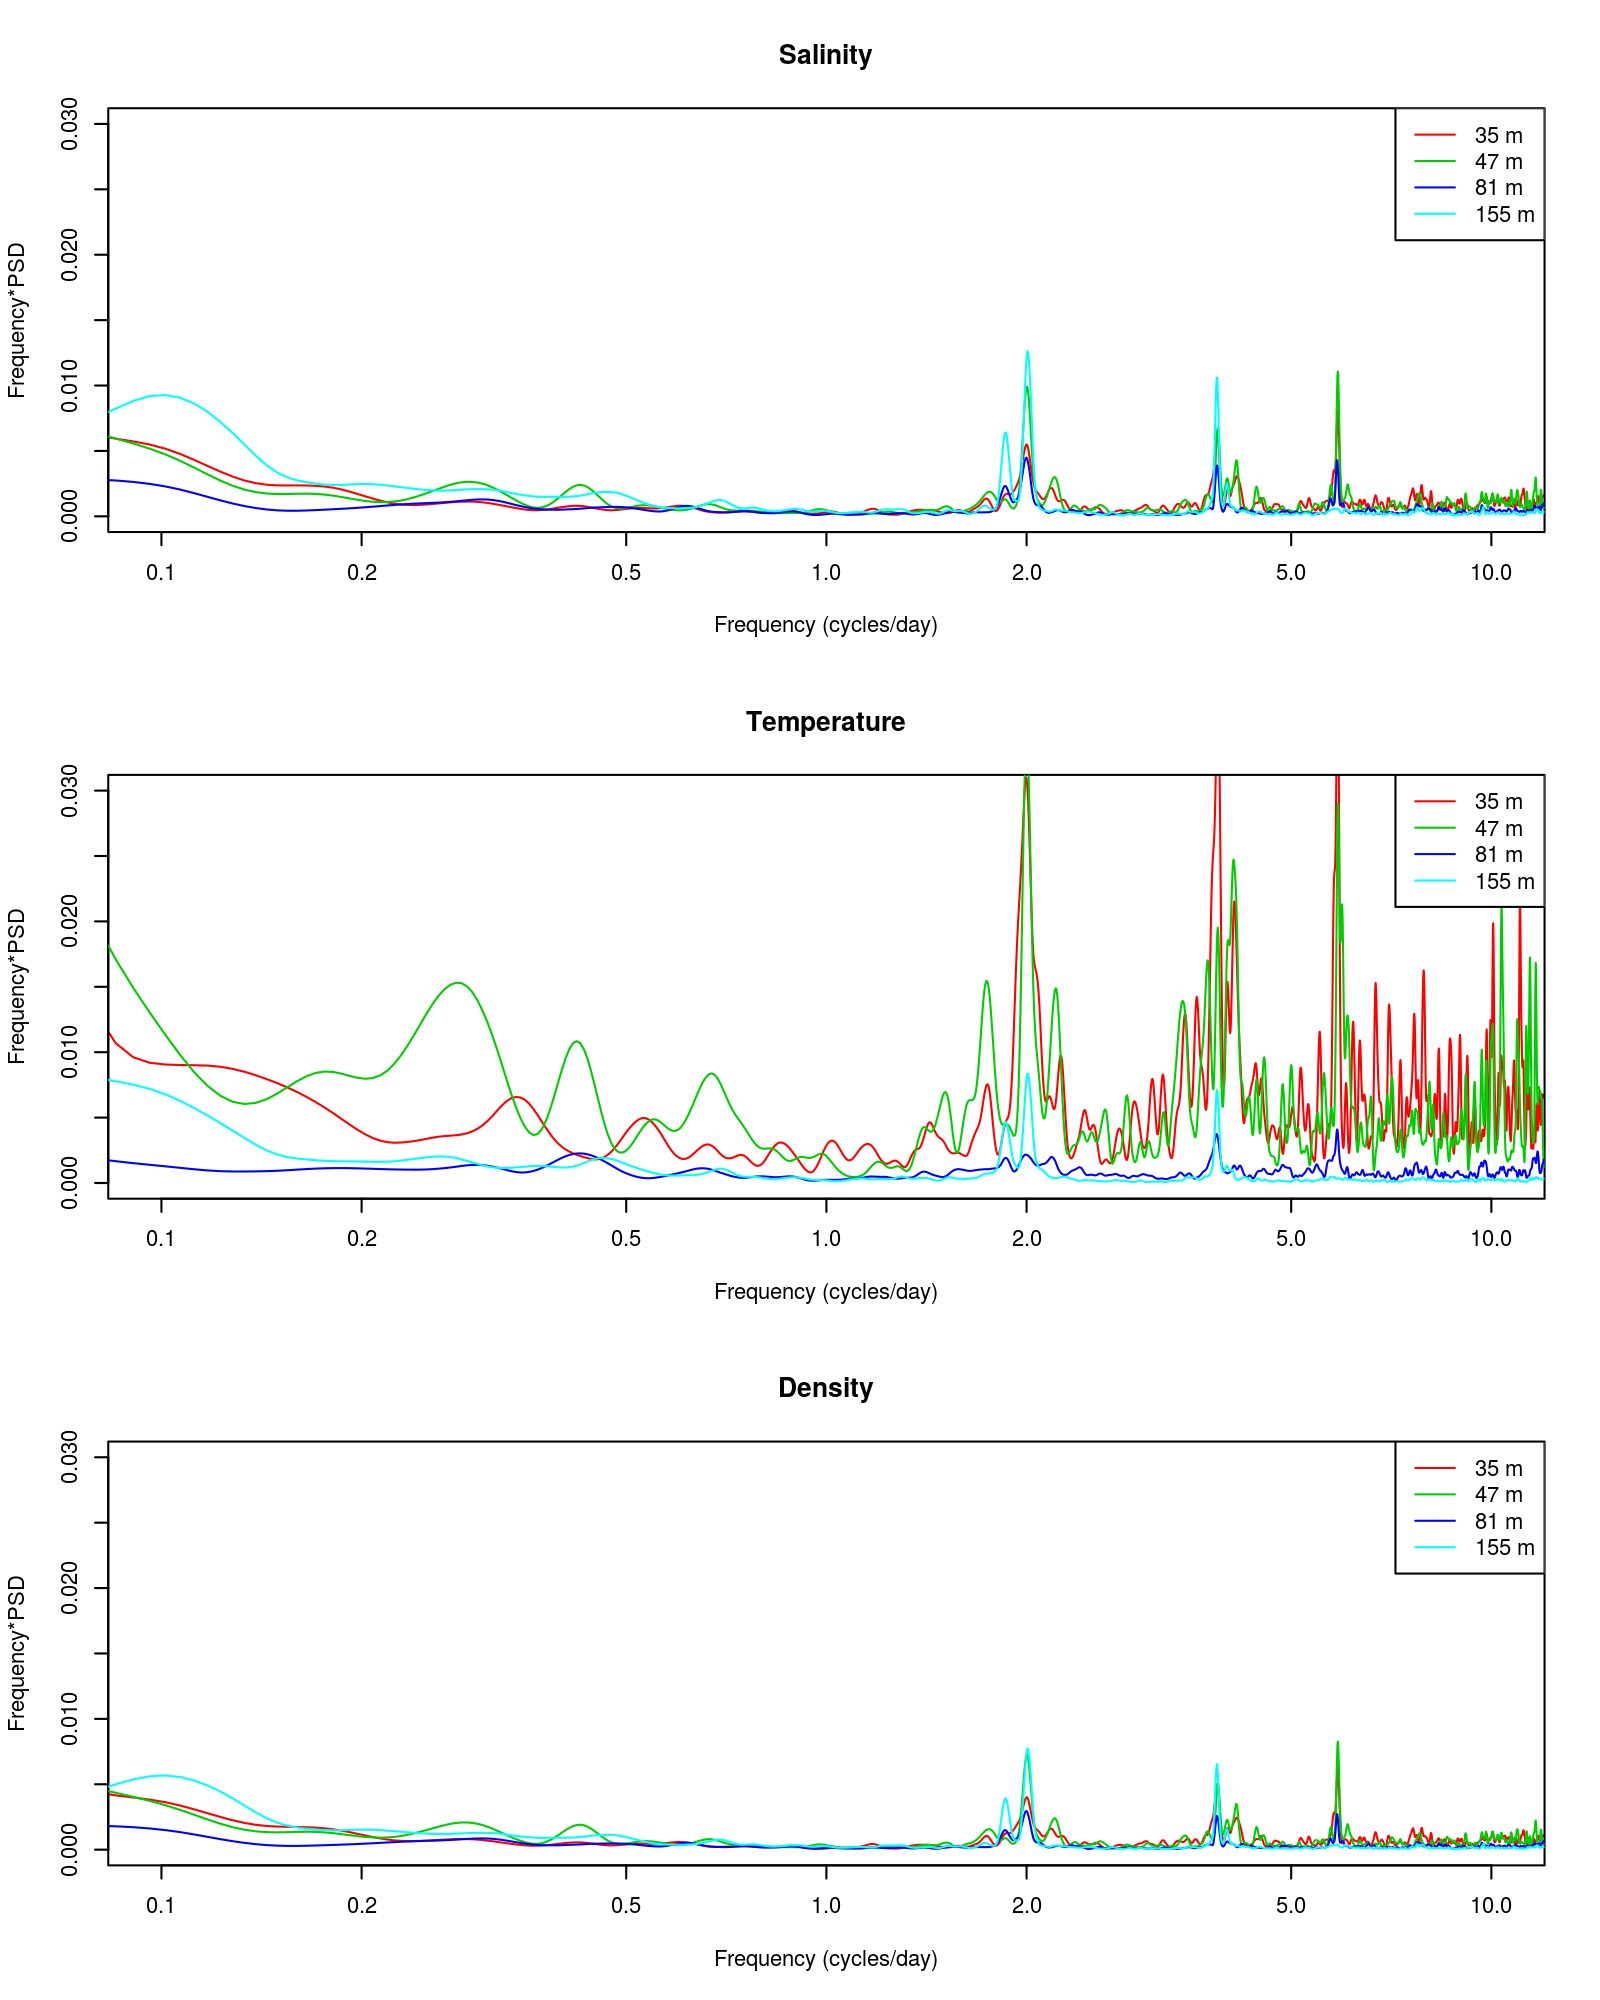
\includegraphics[width = 0.8\textwidth]{./figures/13_mctd_ps_2014_2015.png}
\caption[Power spectra of moored CTD, 2014-2015]{Power spectra of moored CTD data, August 2014 - August 2015.}
\label{f:mctd_ps_2014_2015}
\end{figure}

\begin{figure}  
\centering
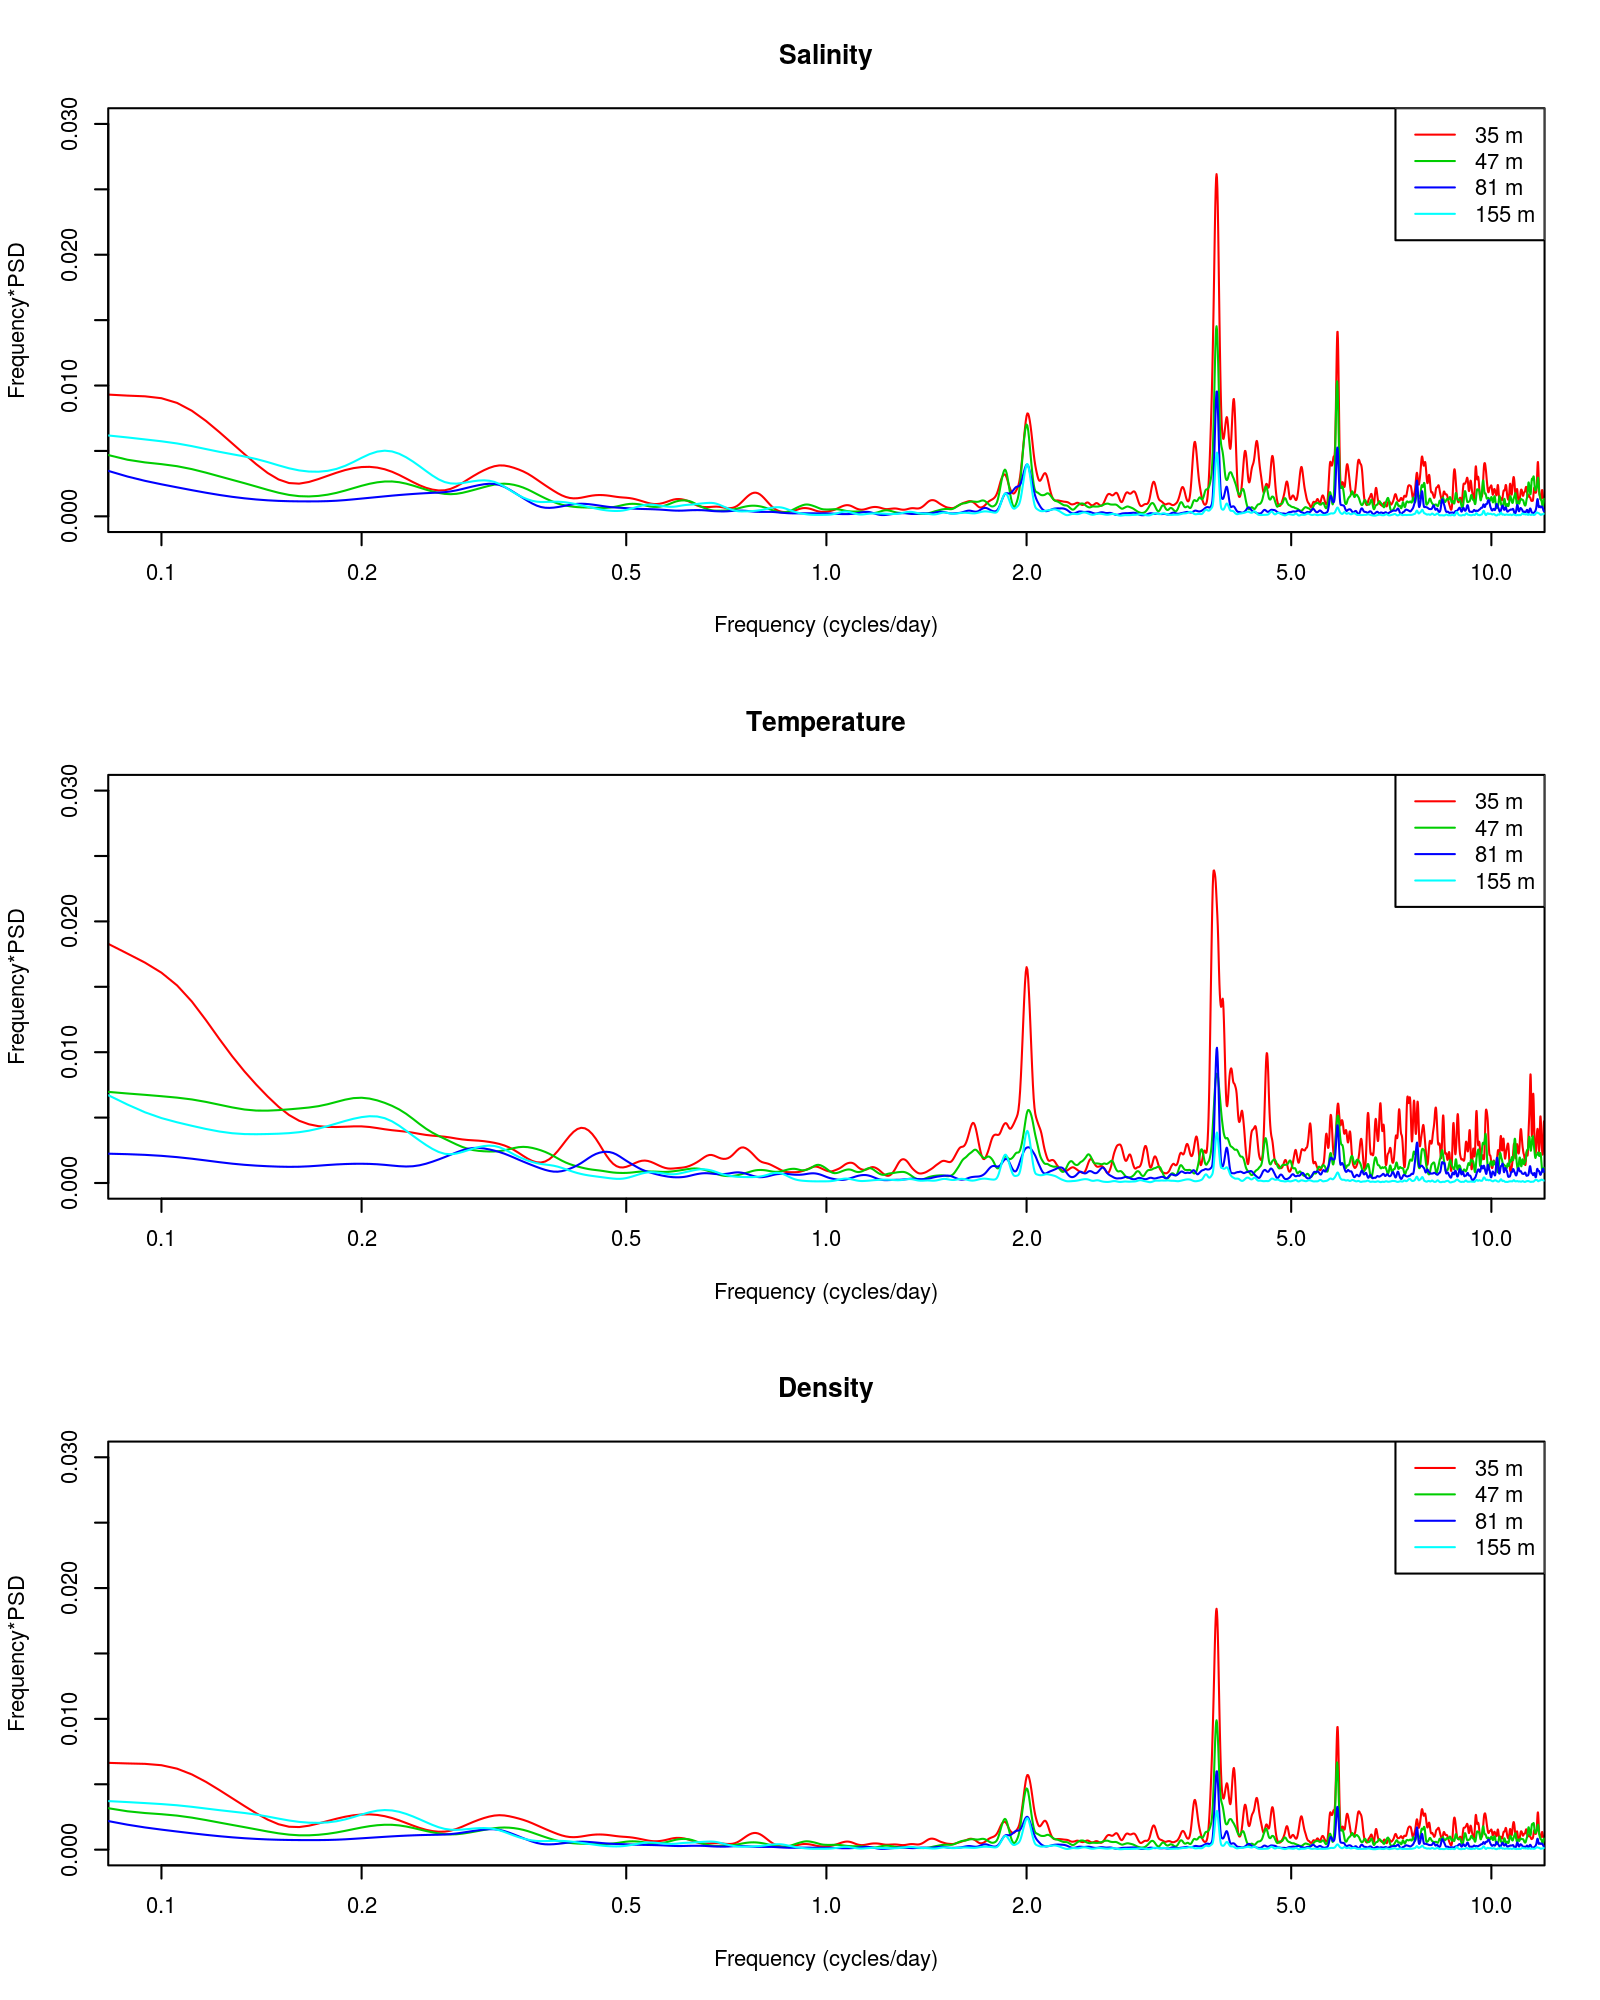
\includegraphics[width = 0.8\textwidth]{./figures/14_mctd_ps_2015_2016.png}
\caption[Power spectra of moored CTD, 2015-2016]{Power spectra of moored CTD data, August 2015 - August 2016.}
\label{f:mctd_ps_2015_2016}
\end{figure}



\begin{figure}  
\centering
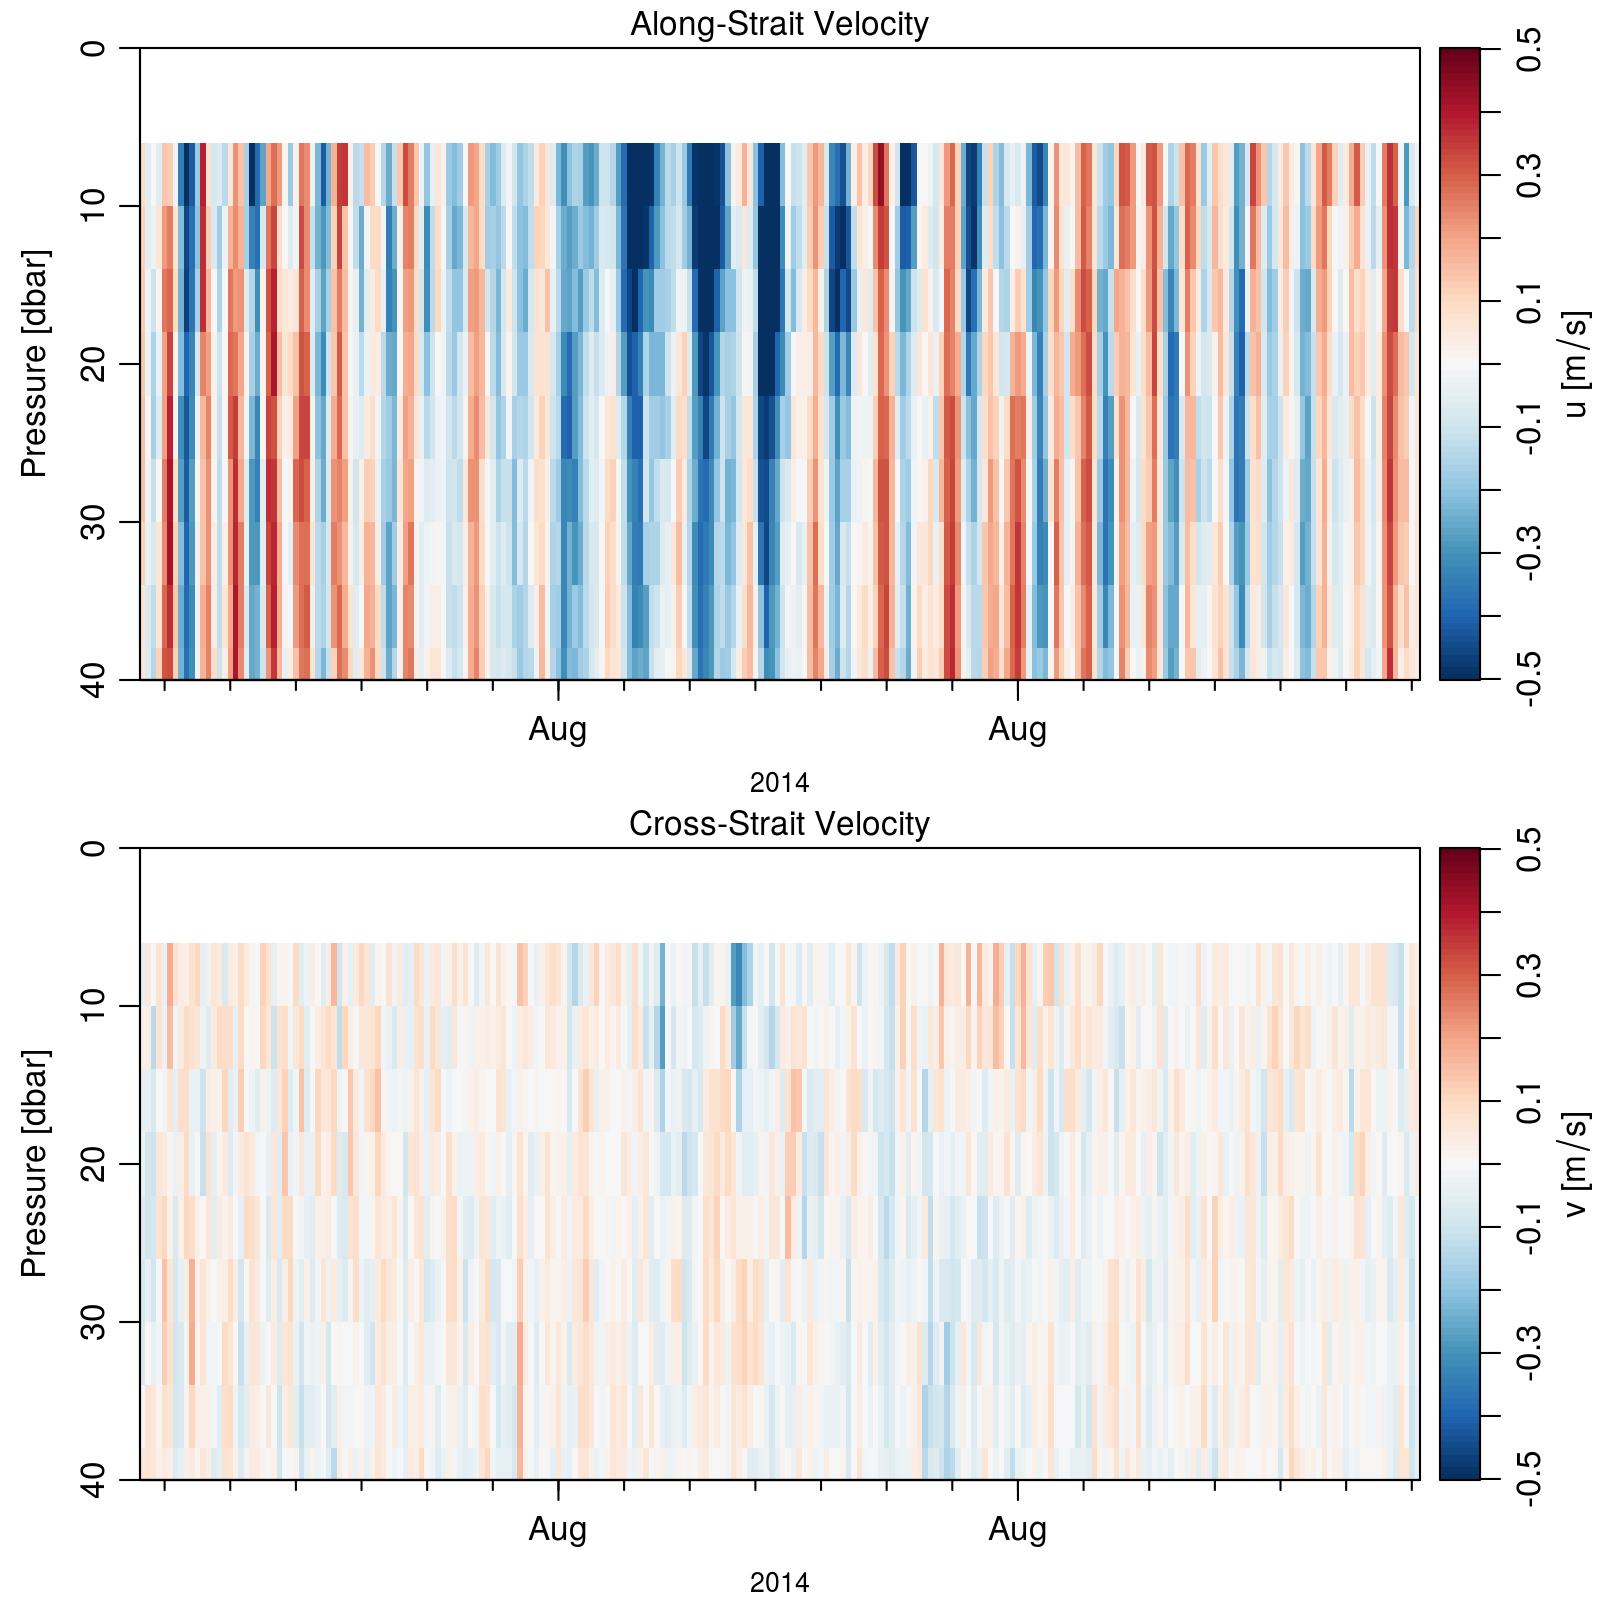
\includegraphics[width = 0.8\textwidth]{./figures/15_madcp_2014.png}
\caption[Bi-hourly ADCP data, Sept. 1 - Sept 20, 2014]{Bi-hourly moored ADCP data, September 1 2014 - September 30 2014.}
\label{f:madcp_sept2014}
\end{figure}

\begin{figure}  
\centering
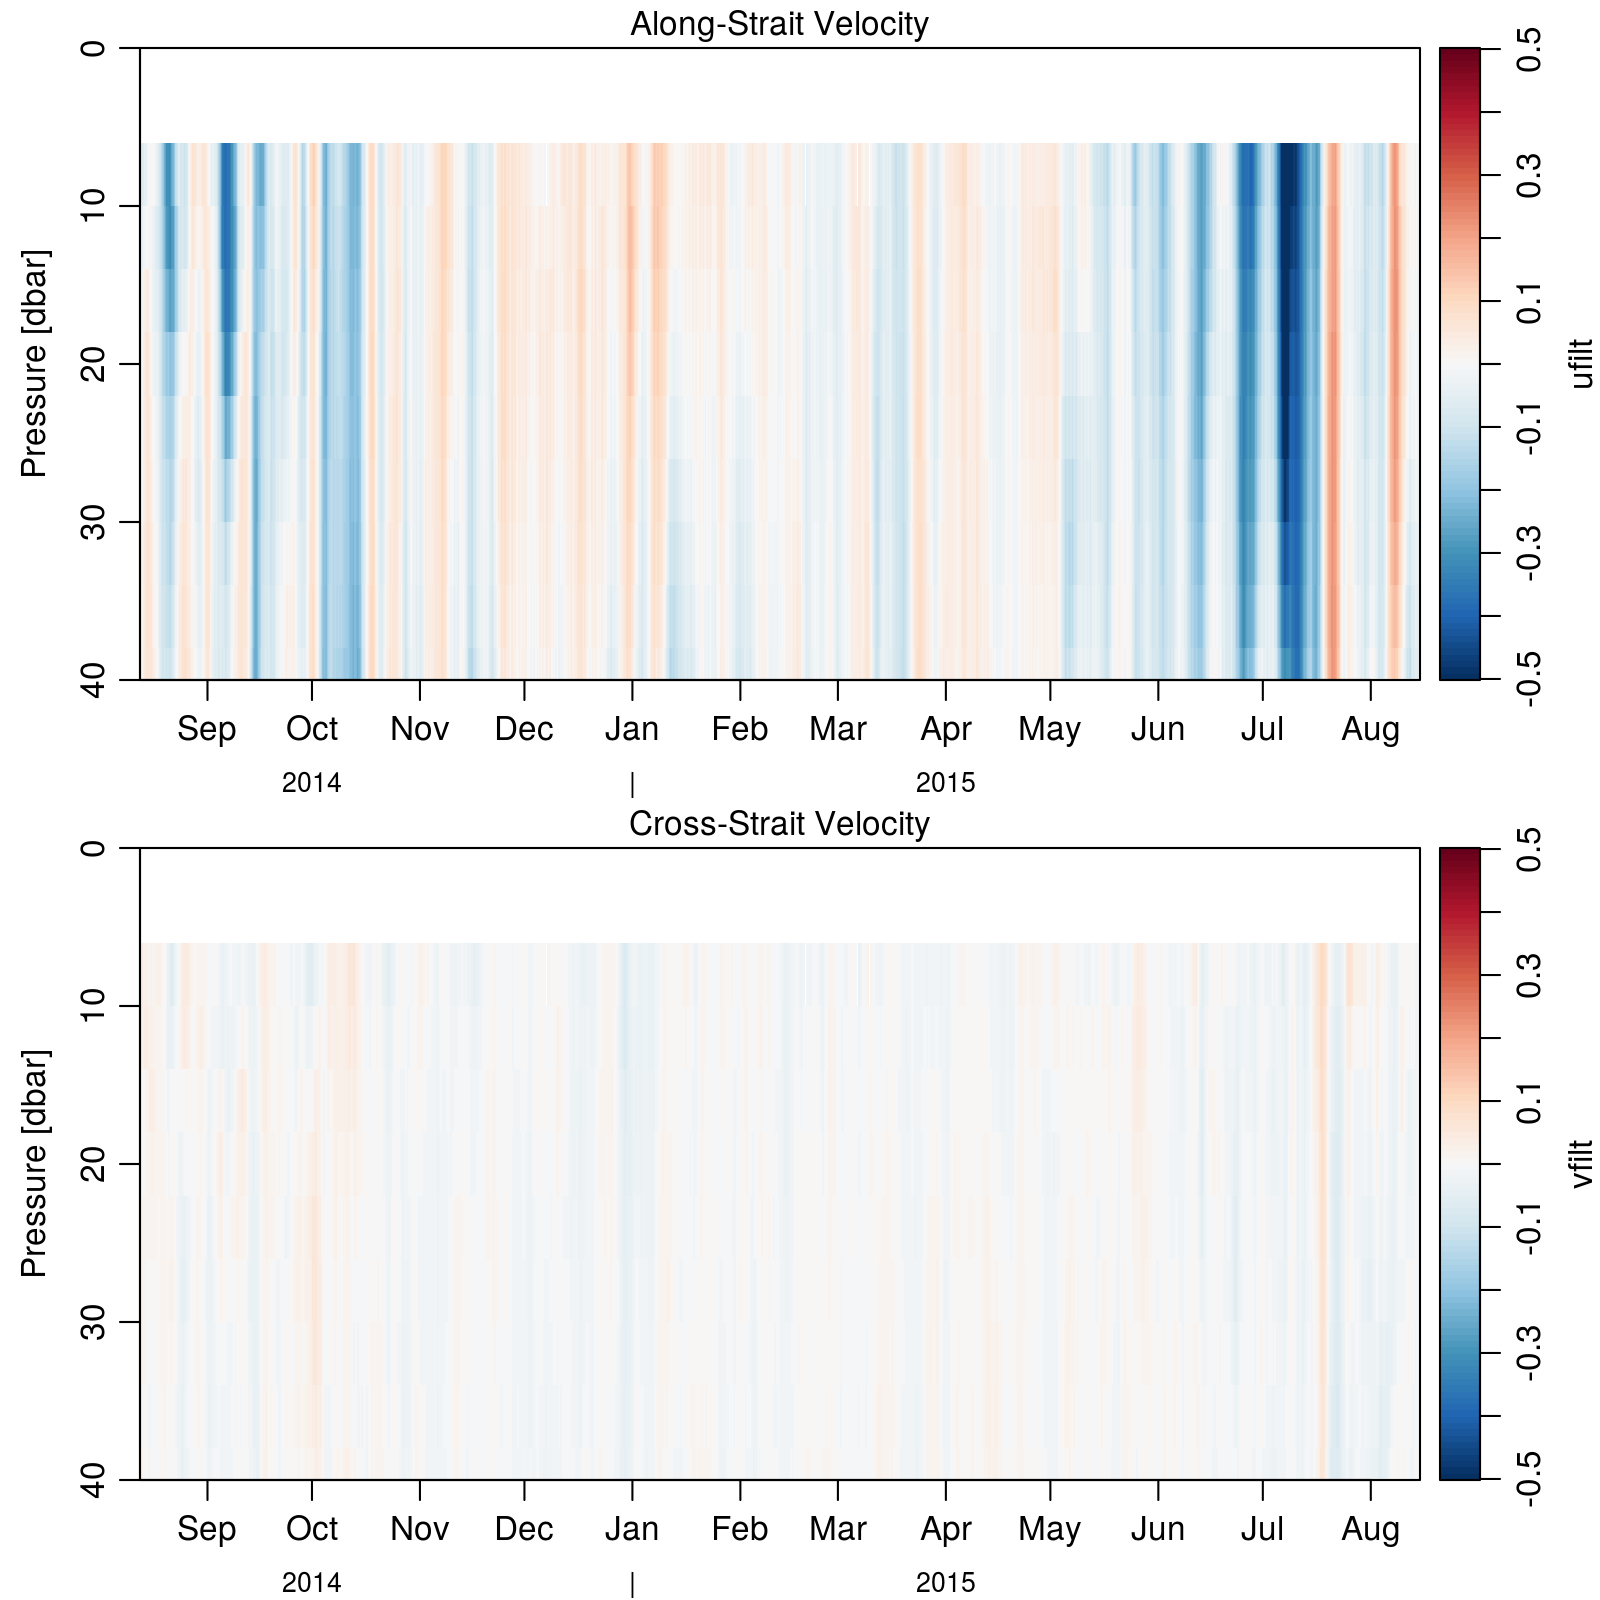
\includegraphics[width = 0.8\textwidth]{./figures/17_madcp_lpf_2014_2015.png}
\caption[Low-pass filtered ADCP data, 2014-2015]{Low-pass filtered ADCP data, August 2014 - August 2015}
\label{f:madcp_lpf_2014_2015}
\end{figure}

\begin{figure}  
\centering
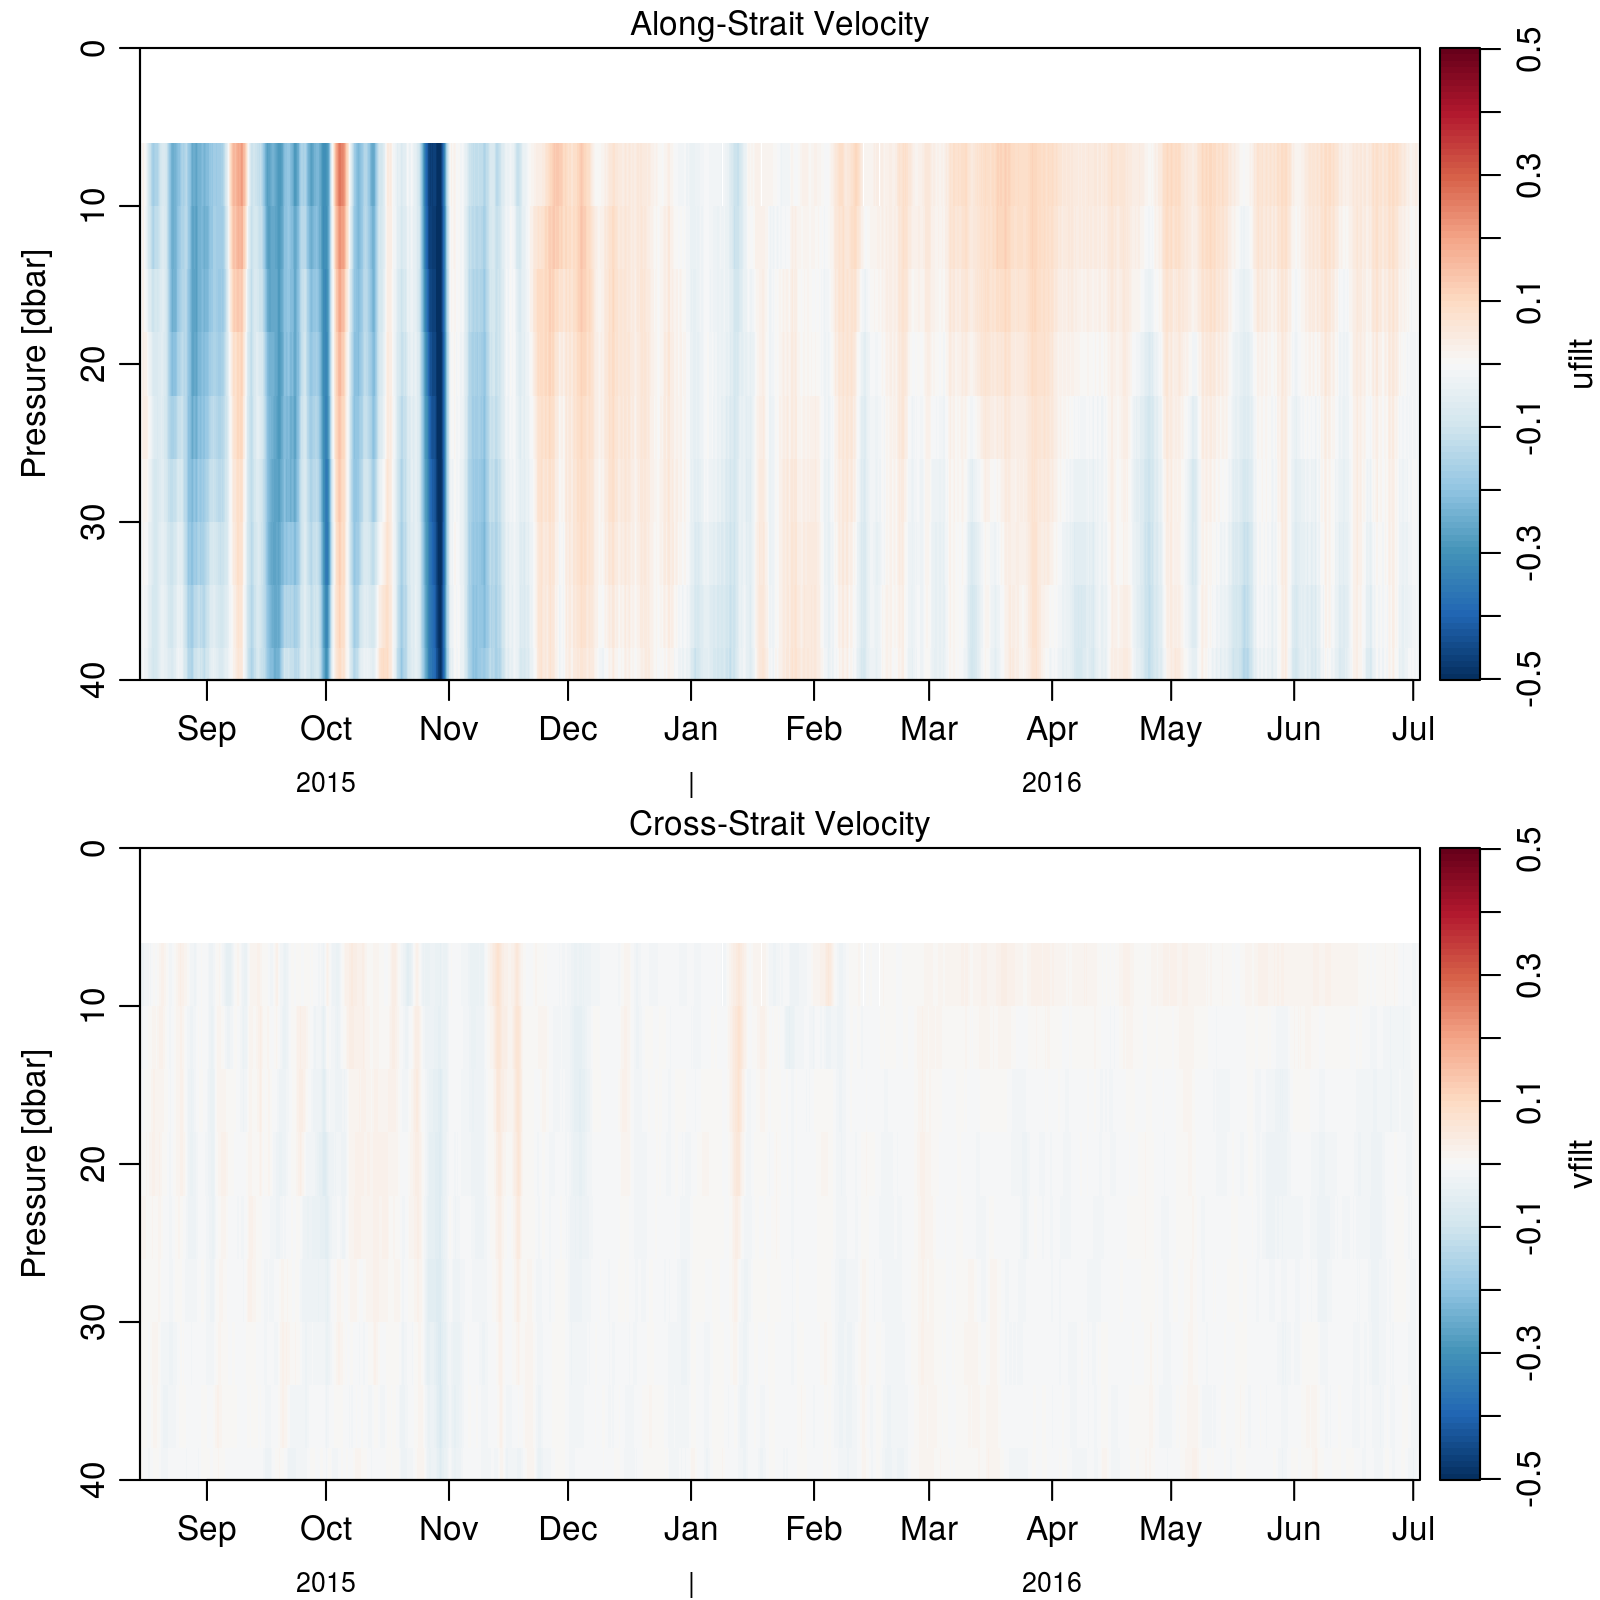
\includegraphics[width = 0.8\textwidth]{./figures/18_madcp_lpf_2015_2016.png}
\caption[Low-pass filtered ADCP data, 2015-2016]{Low-pass filtered ADCP data, August 2015 - August 2016}
\label{f:madcp_lpf_2015_2016}
\end{figure}



\begin{figure}  
\centering
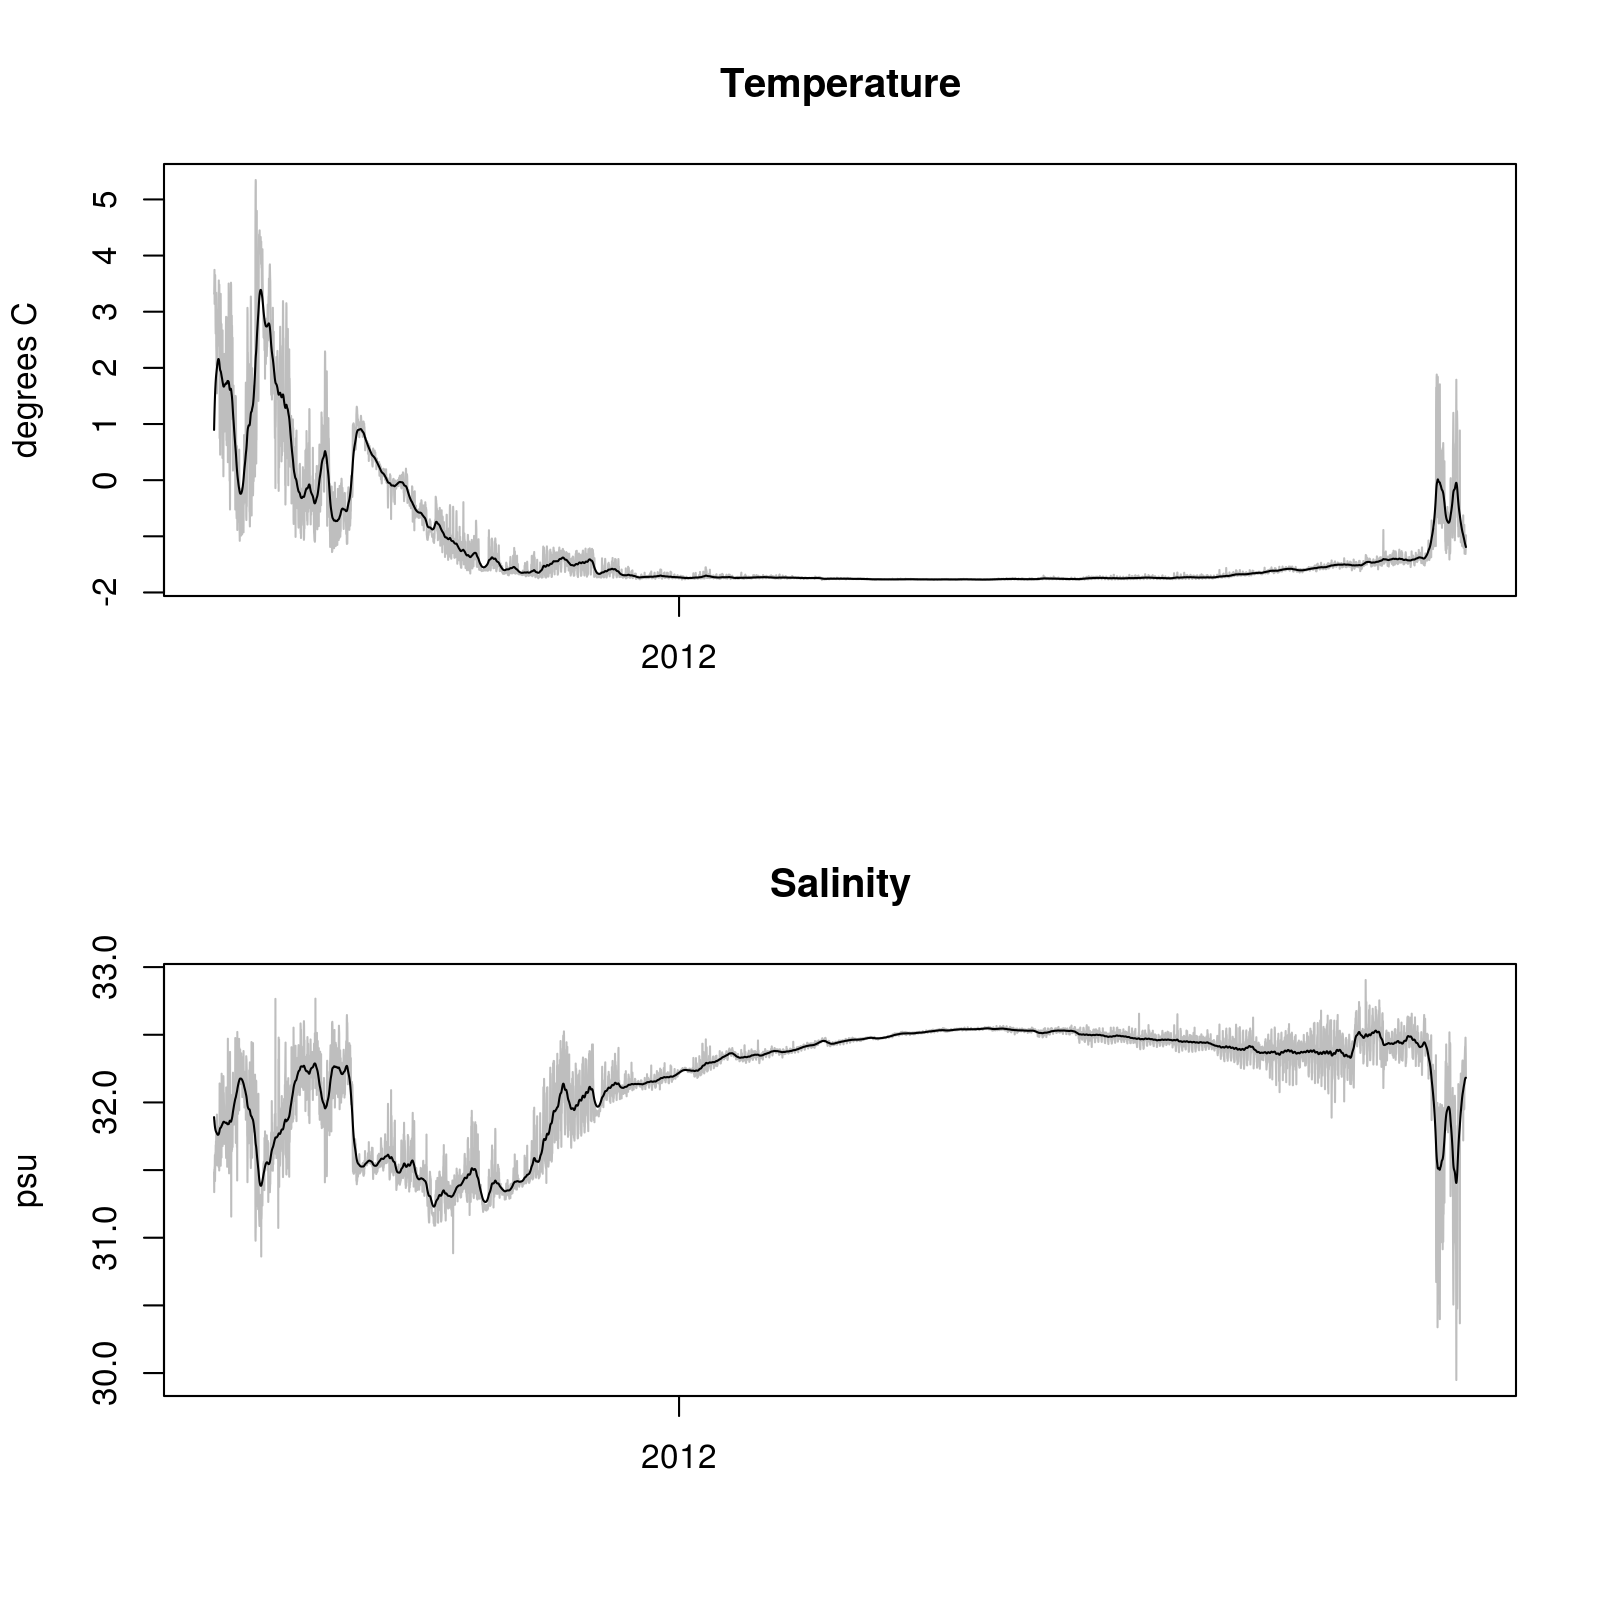
\includegraphics[width = 0.8\textwidth]{./figures/19_lpf_TS_43m_2011_2012.png}
\caption[Low-pass filtered T, S (43 m), 2011-2012]{Low-pass filtered T, S (43 m), August 2011 - August 2012}
\label{f:ctd_43_lpf_2011_2012}
\end{figure}

\begin{figure}  
\centering
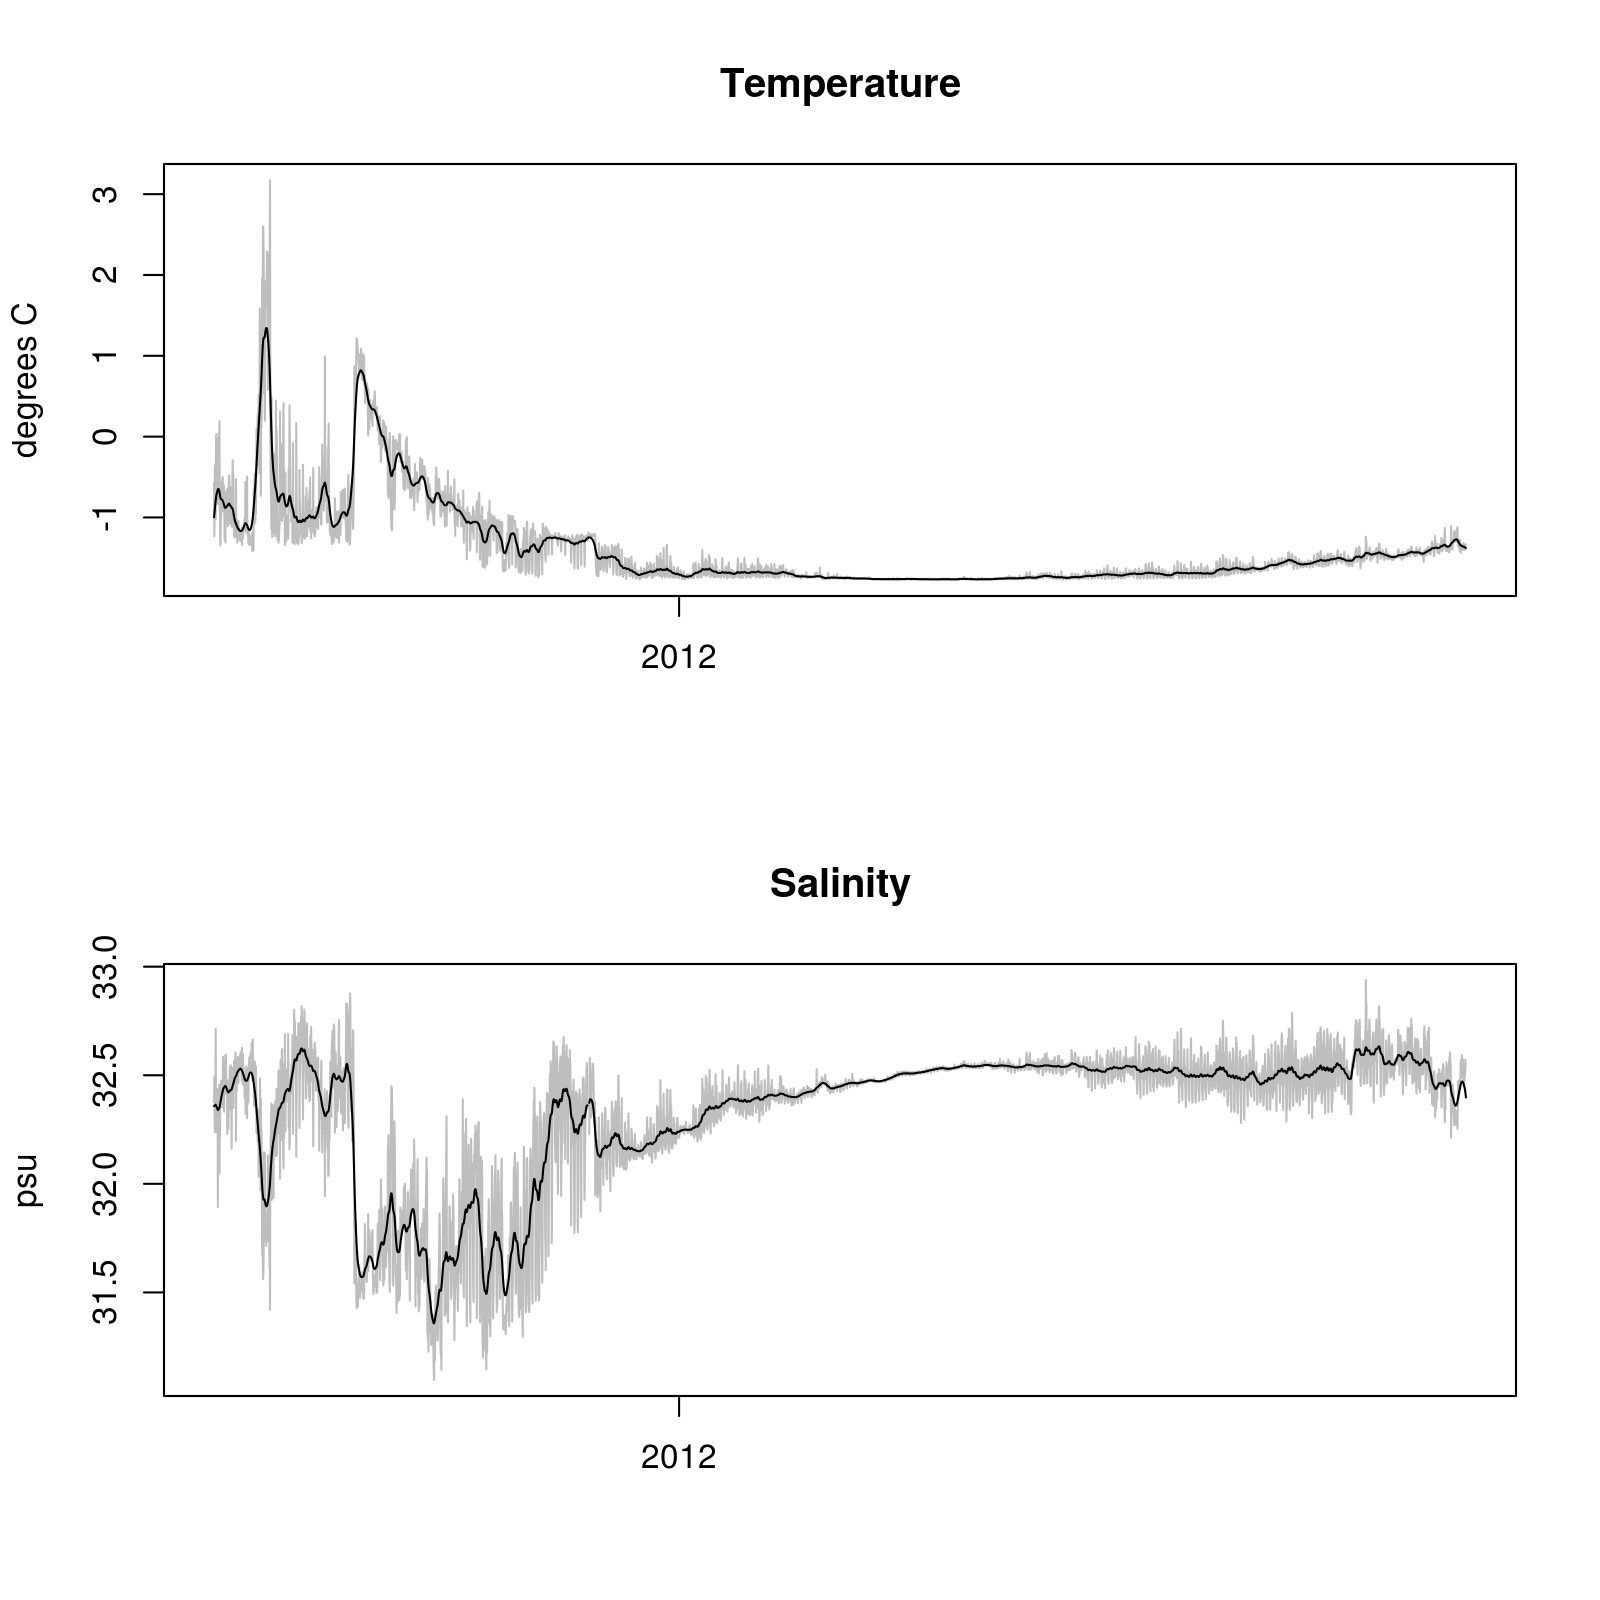
\includegraphics[width = 0.8\textwidth]{./figures/20_lpf_TS_63m_2011_2012.png}
\caption[Low-pass filtered T, S (63 m), 2011-2012]{Low-pass filtered T, S (63 m), August 2011 - August 2012}
\label{f:ctd_63_lpf_2011_2012}
\end{figure}

\begin{figure}  
\centering
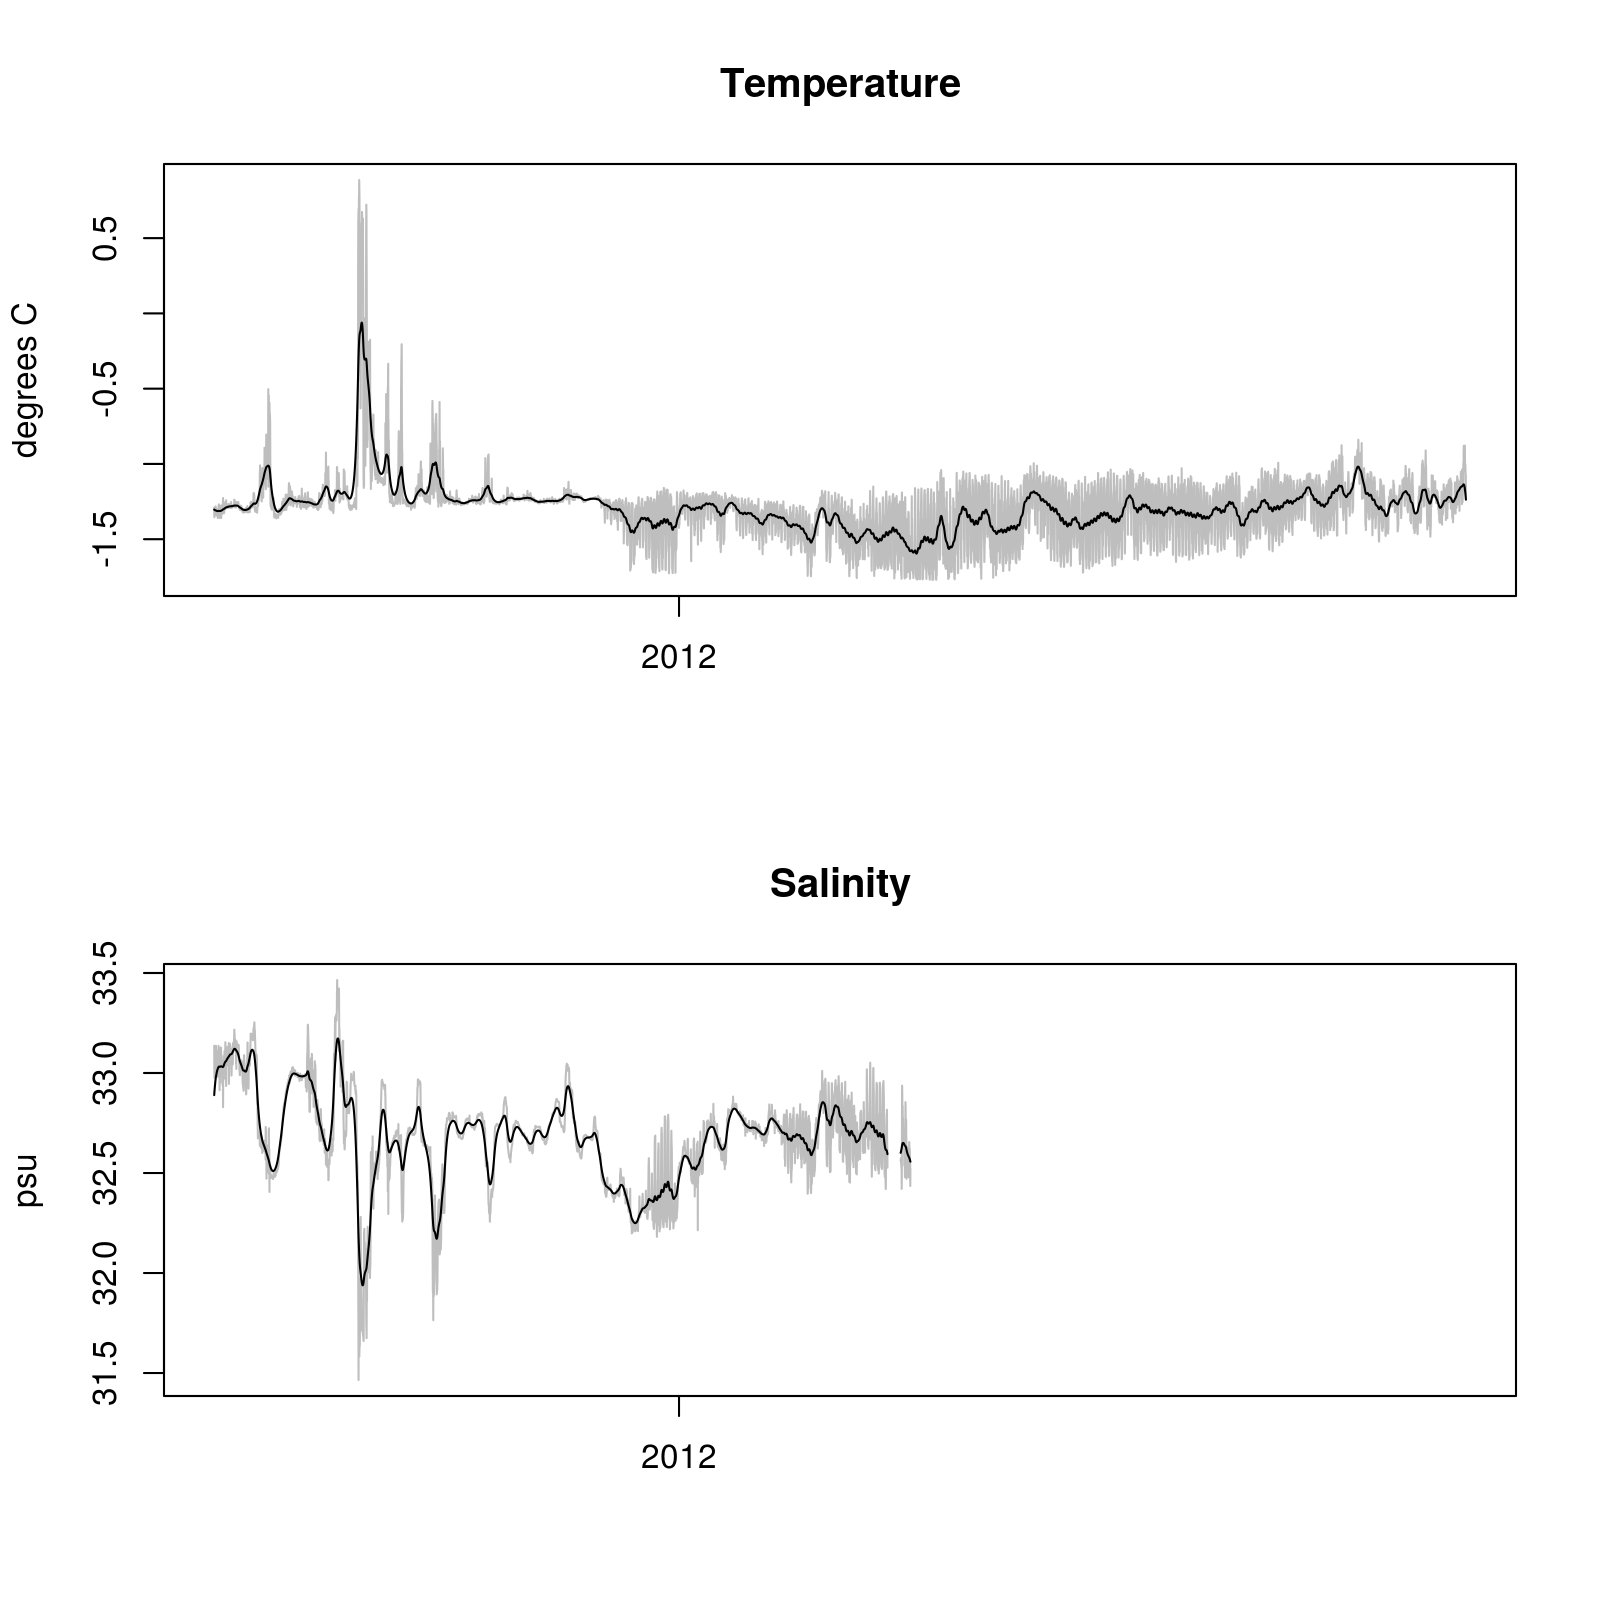
\includegraphics[width = 0.8\textwidth]{./figures/21_lpf_TS_120m_2011_2012.png}
\caption[Low-pass filtered T, S (120 m), 2011-2012]{Low-pass filtered T, S (120 m), August 2011 - August 2012}
\label{f:ctd_120_lpf_2011_2012}
\end{figure}


\begin{figure}  
\centering
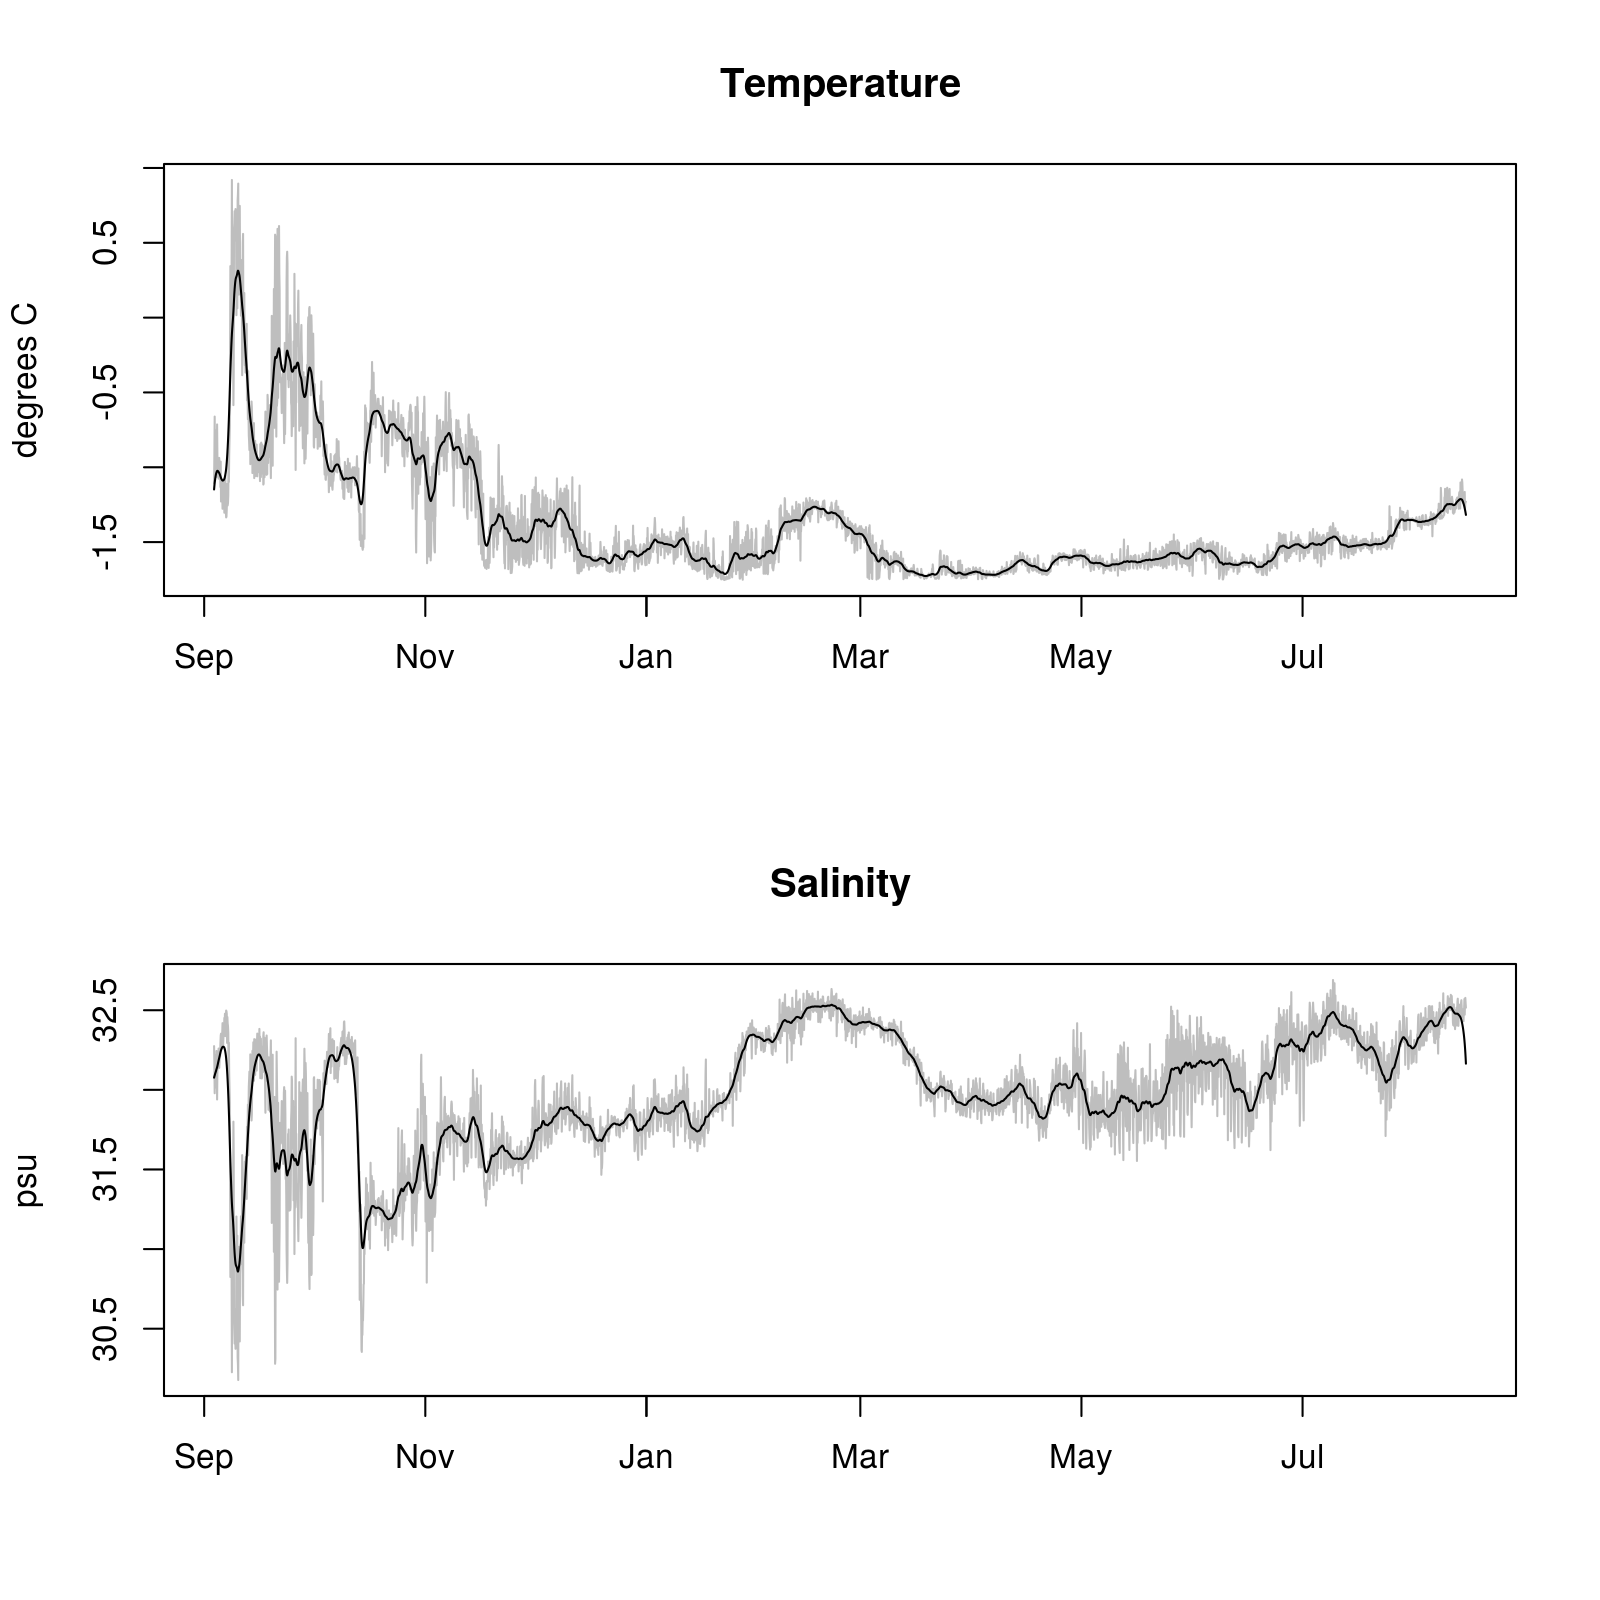
\includegraphics[width = 0.8\textwidth]{./figures/22_lpf_TS_41m_2012_2013.png}
\caption[Low-pass filtered T, S (41 m), 2012-2013]{Low-pass filtered T, S (41 m), August 2012 - August 2013}
\label{f:ctd_41_lpf_2012_2013}
\end{figure}

\begin{figure}  
\centering
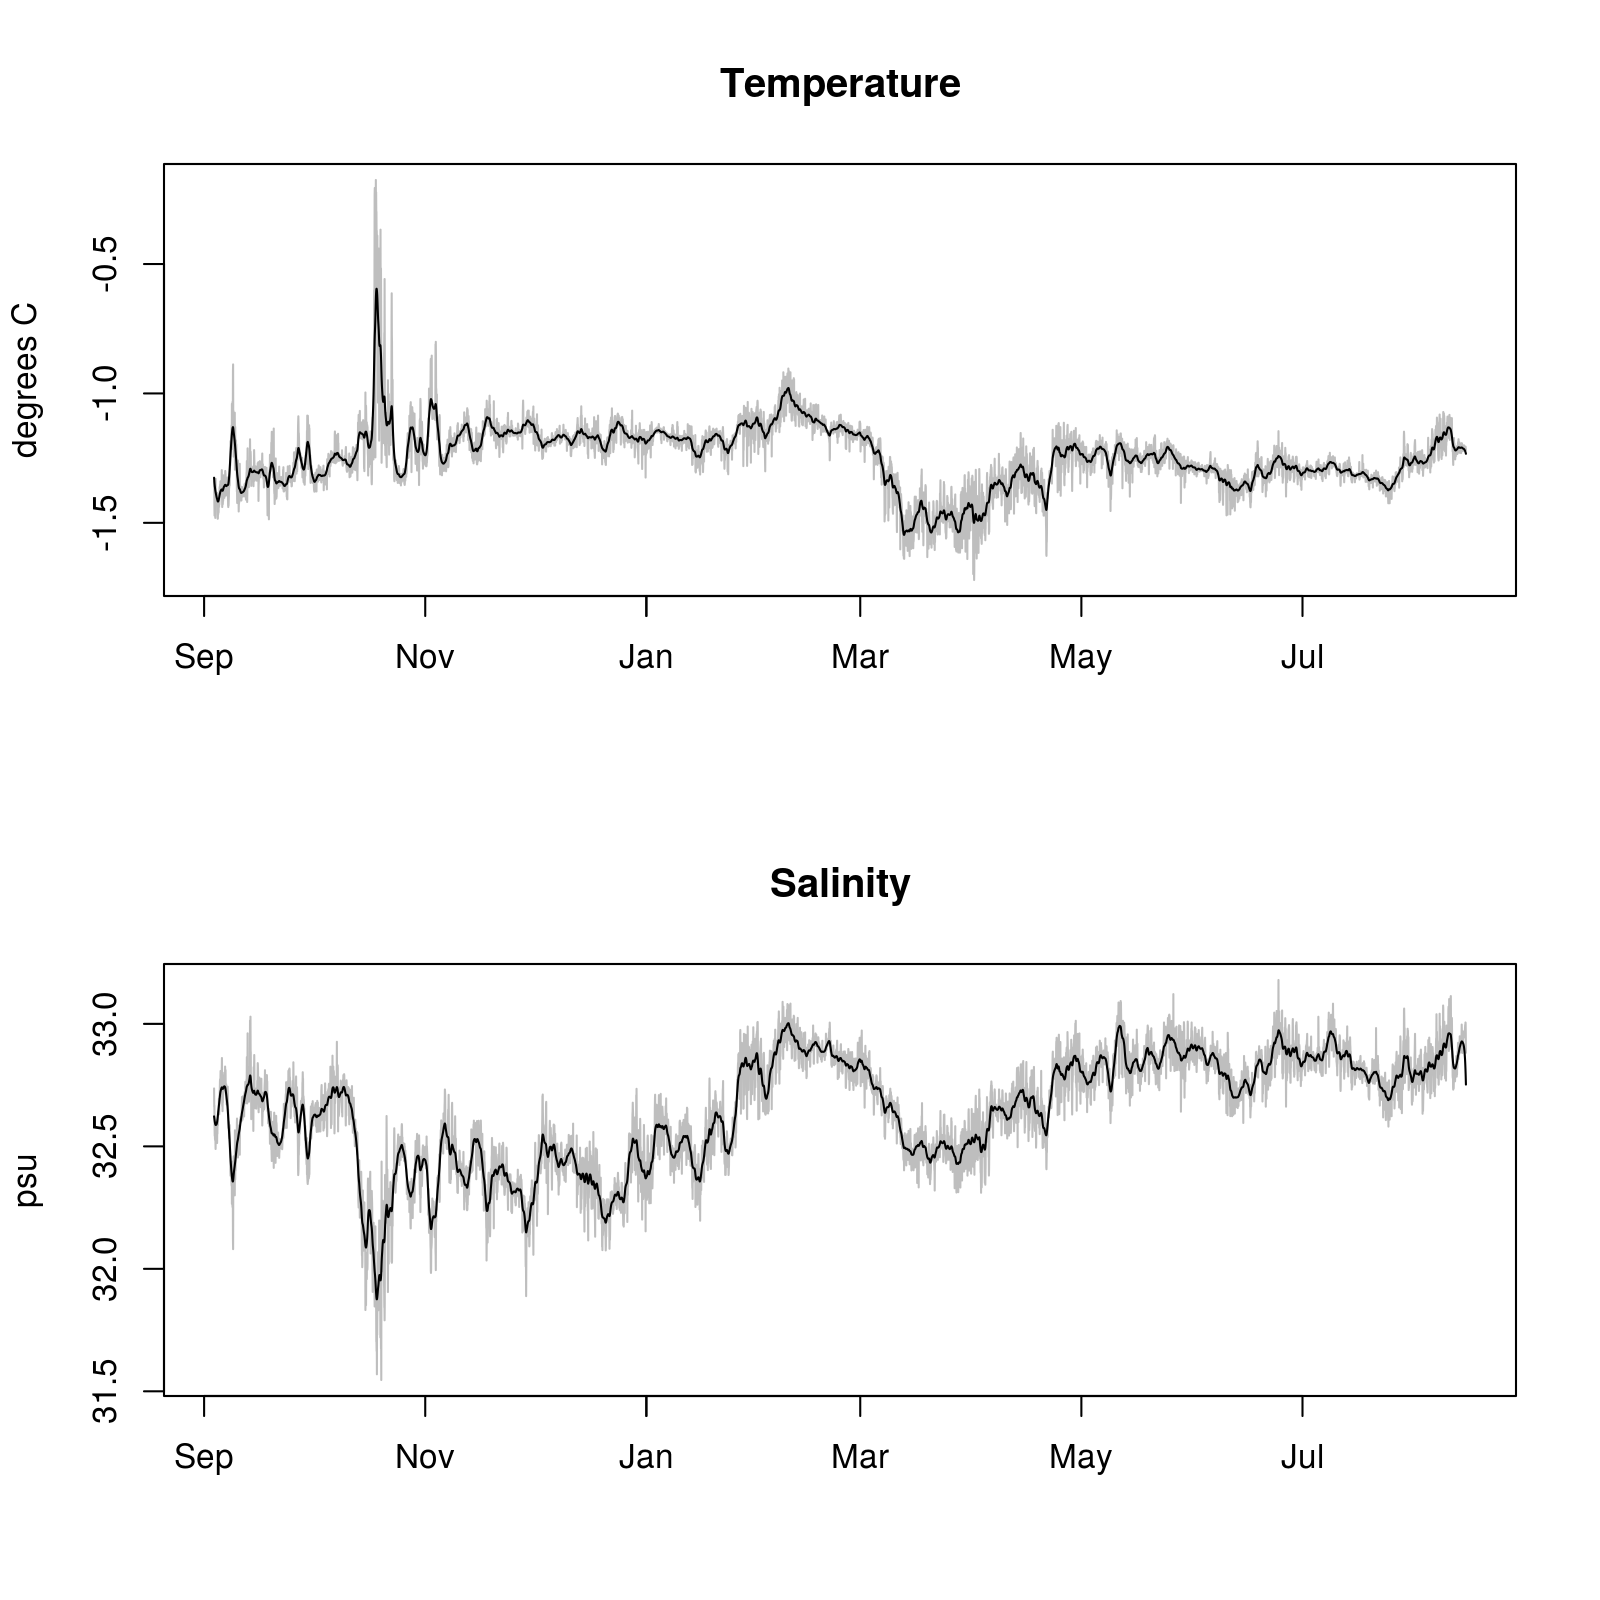
\includegraphics[width = 0.8\textwidth]{./figures/23_lpf_TS_81m_2012_2013.png}
\caption[Low-pass filtered T, S (81 m), 2012-2013]{Low-pass filtered T, S (81 m), August 2012 - August 2013}
\label{f:ctd_81_lpf_2012_2013}
\end{figure}

\begin{figure}  
\centering
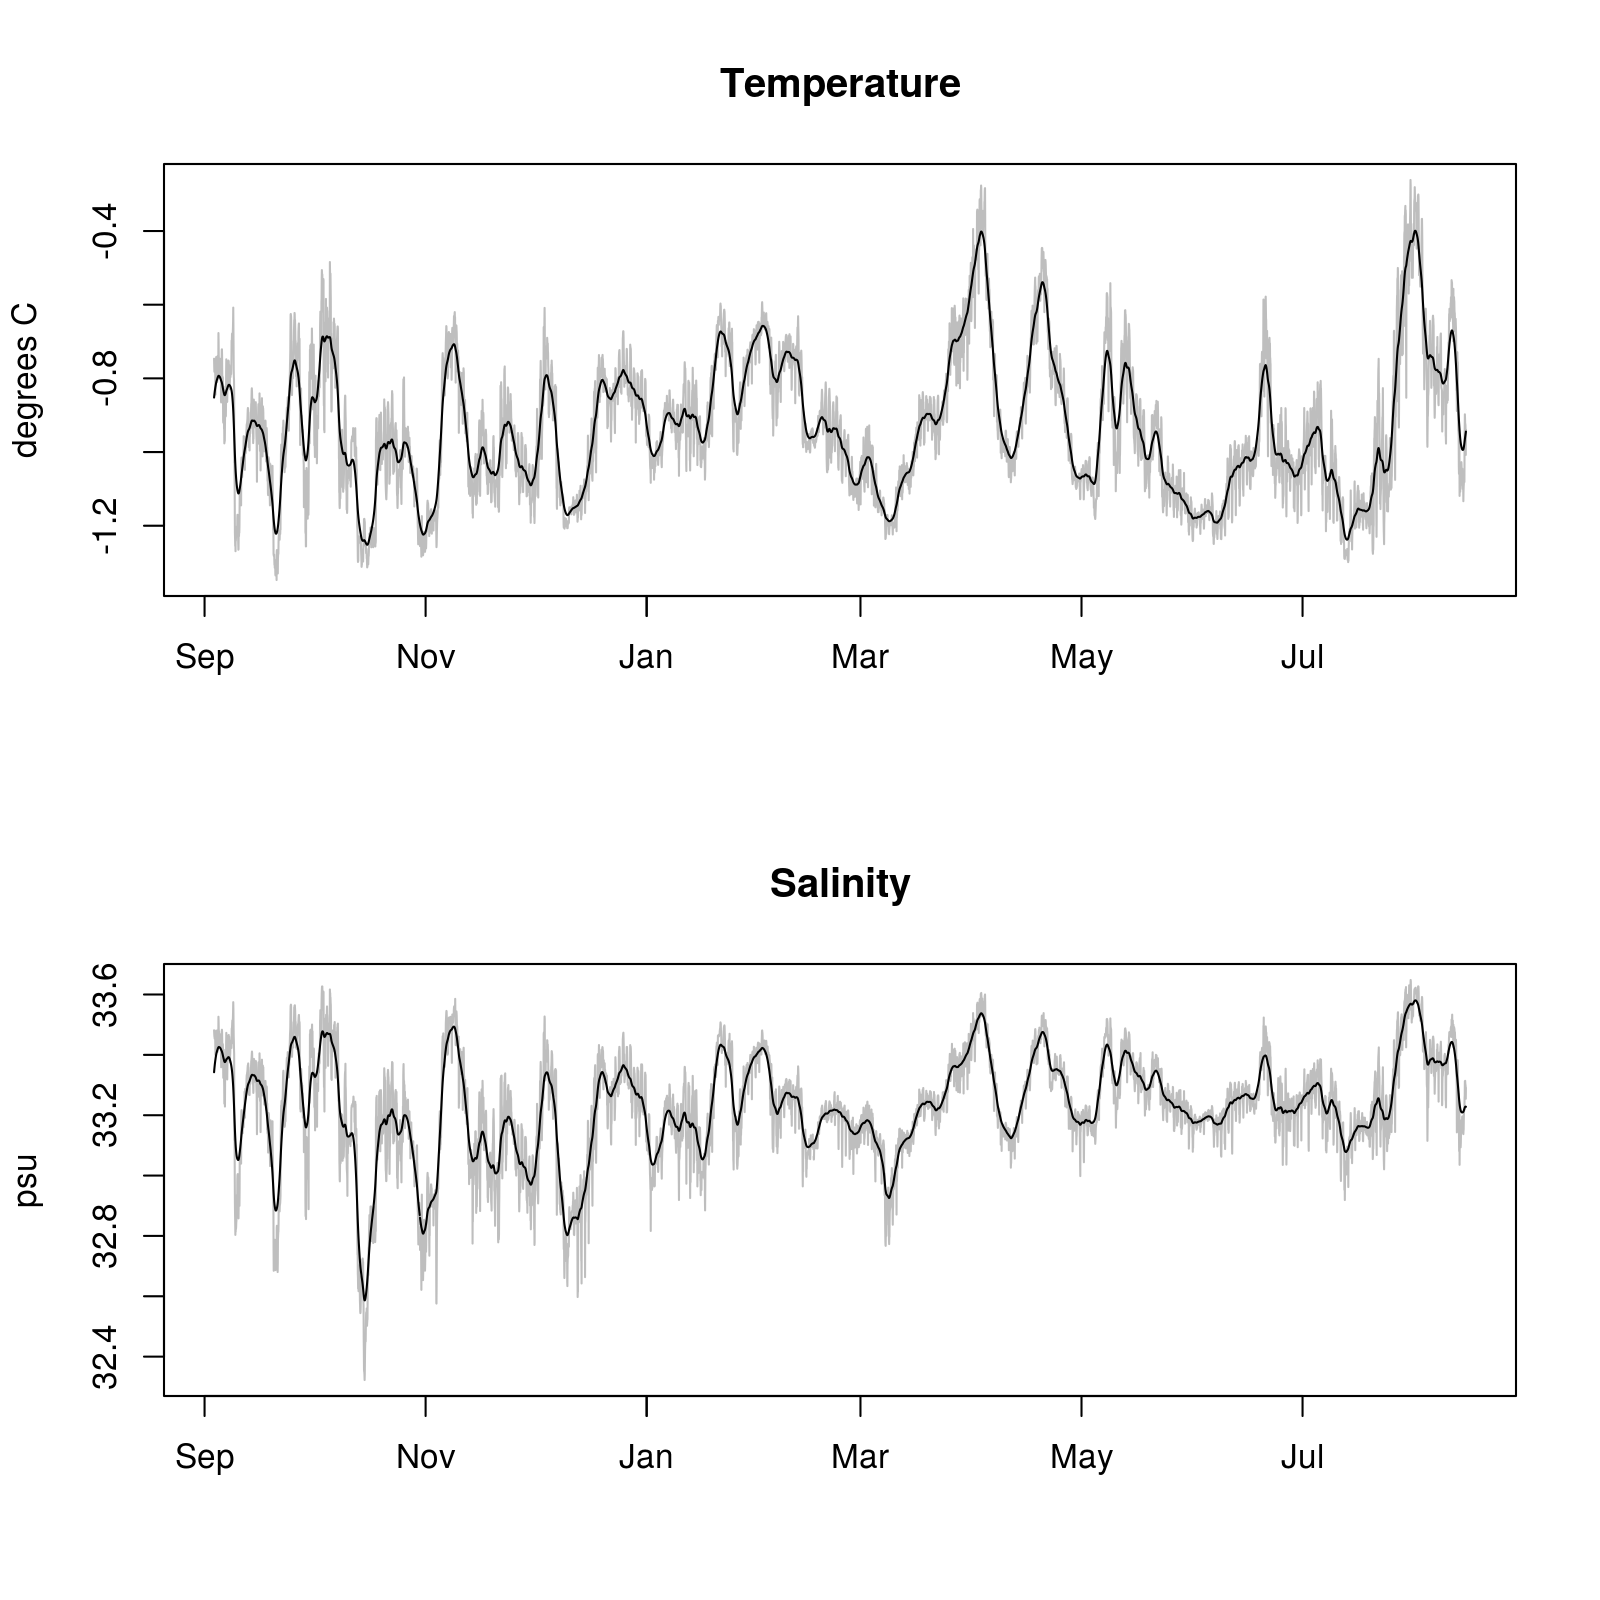
\includegraphics[width = 0.8\textwidth]{./figures/24_lpf_TS_155m_2012_2013.png}
\caption[Low-pass filtered T, S (155 m), 2012-2013]{Low-pass filtered T, S (155 m), August 2012 - August 2013}
\label{f:ctd_155_lpf_2012_2013}
\end{figure}


\begin{figure}  
\centering
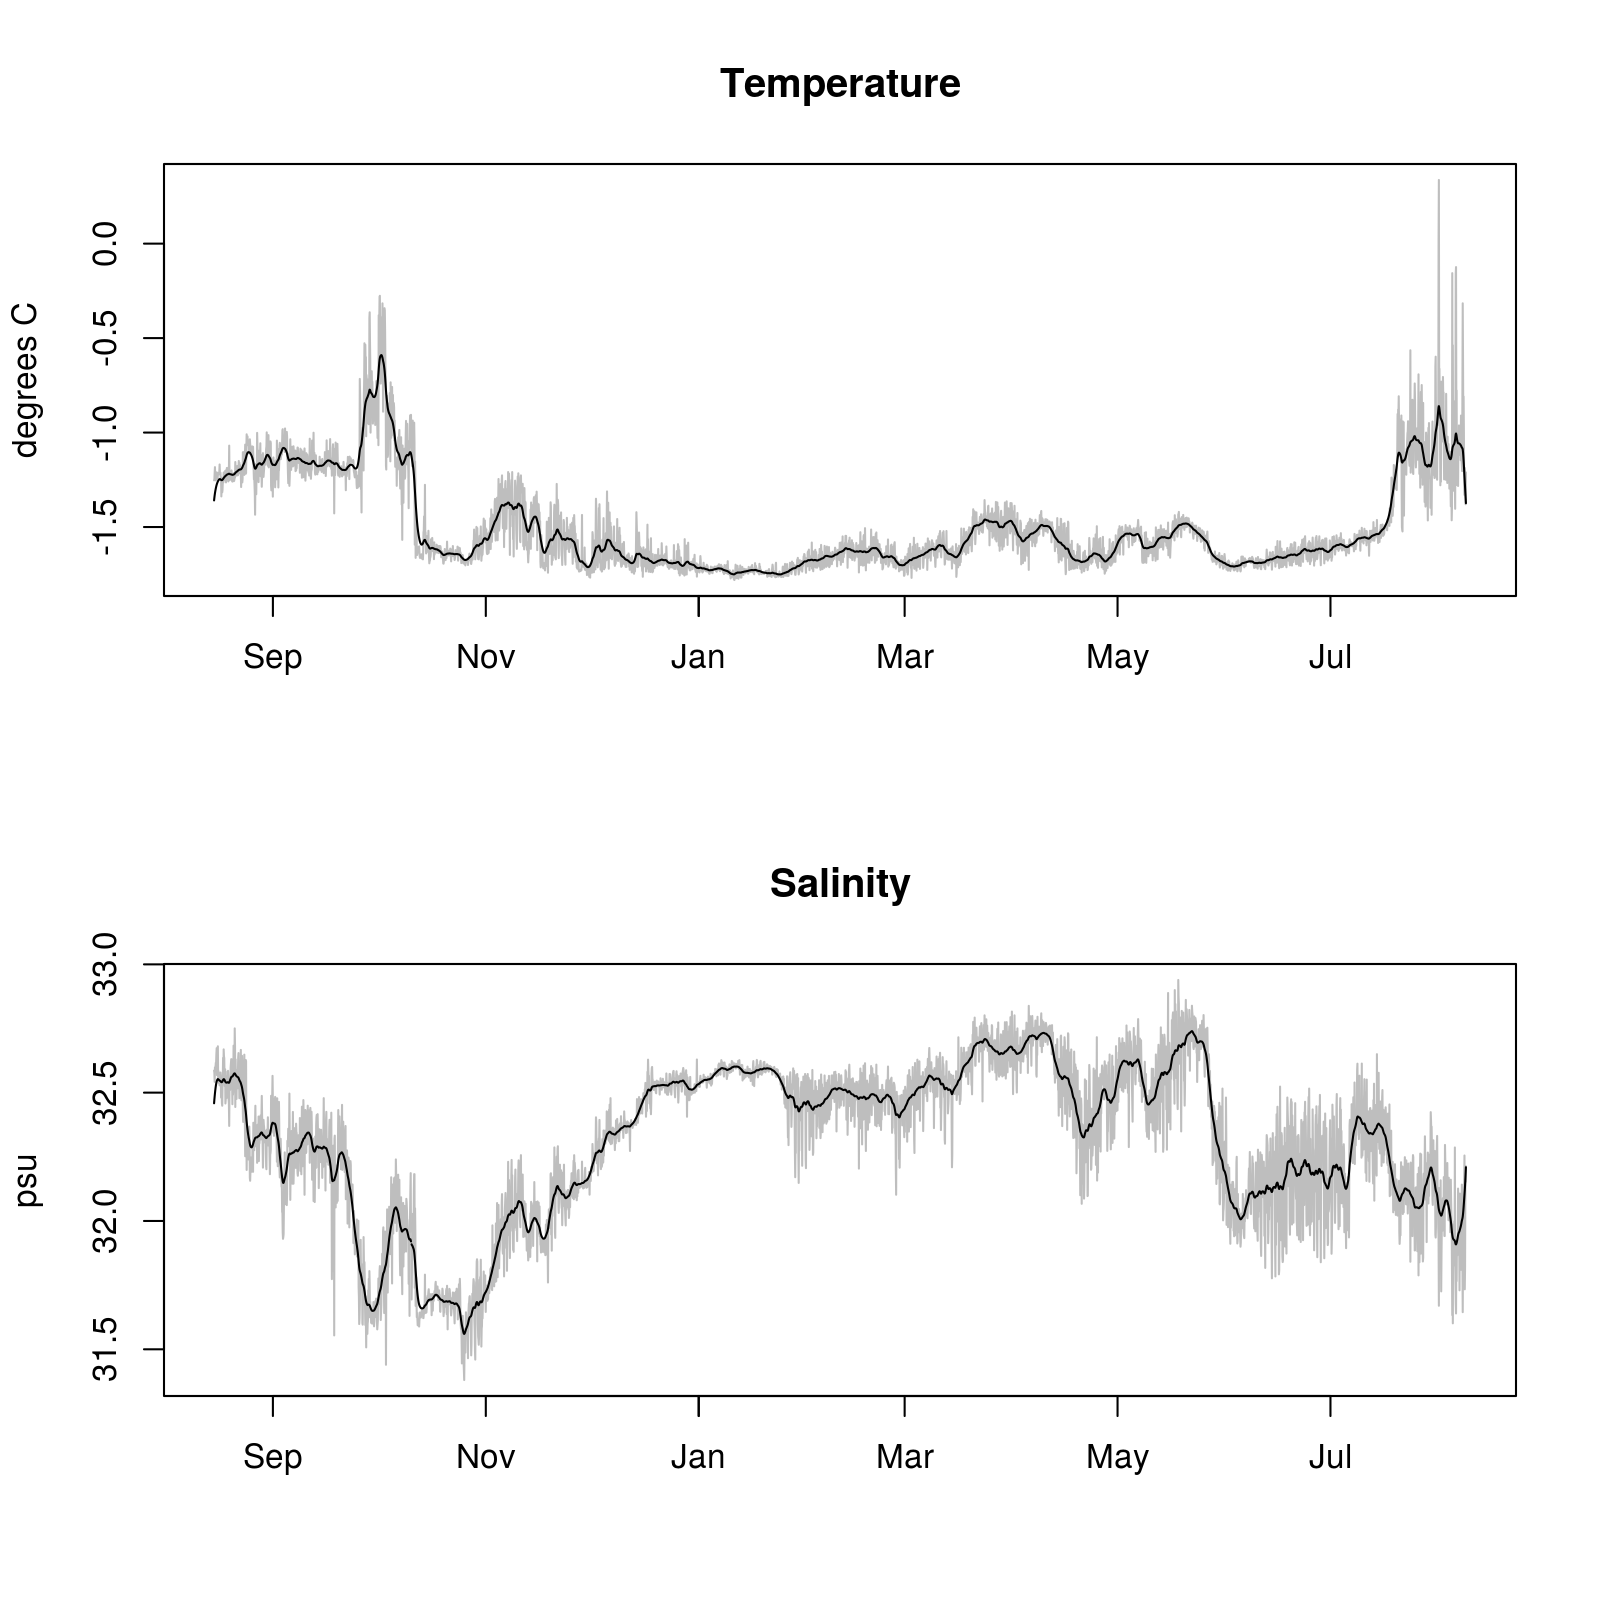
\includegraphics[width = 0.8\textwidth]{./figures/25_lpf_TS_41m_2013_2014.png}
\caption[Low-pass filtered T, S (41 m), 2013-2014]{Low-pass filtered T, S (41 m), August 2013 - August 2014}
\label{f:ctd_41_lpf_2013_2014}
\end{figure}

\begin{figure}  
\centering
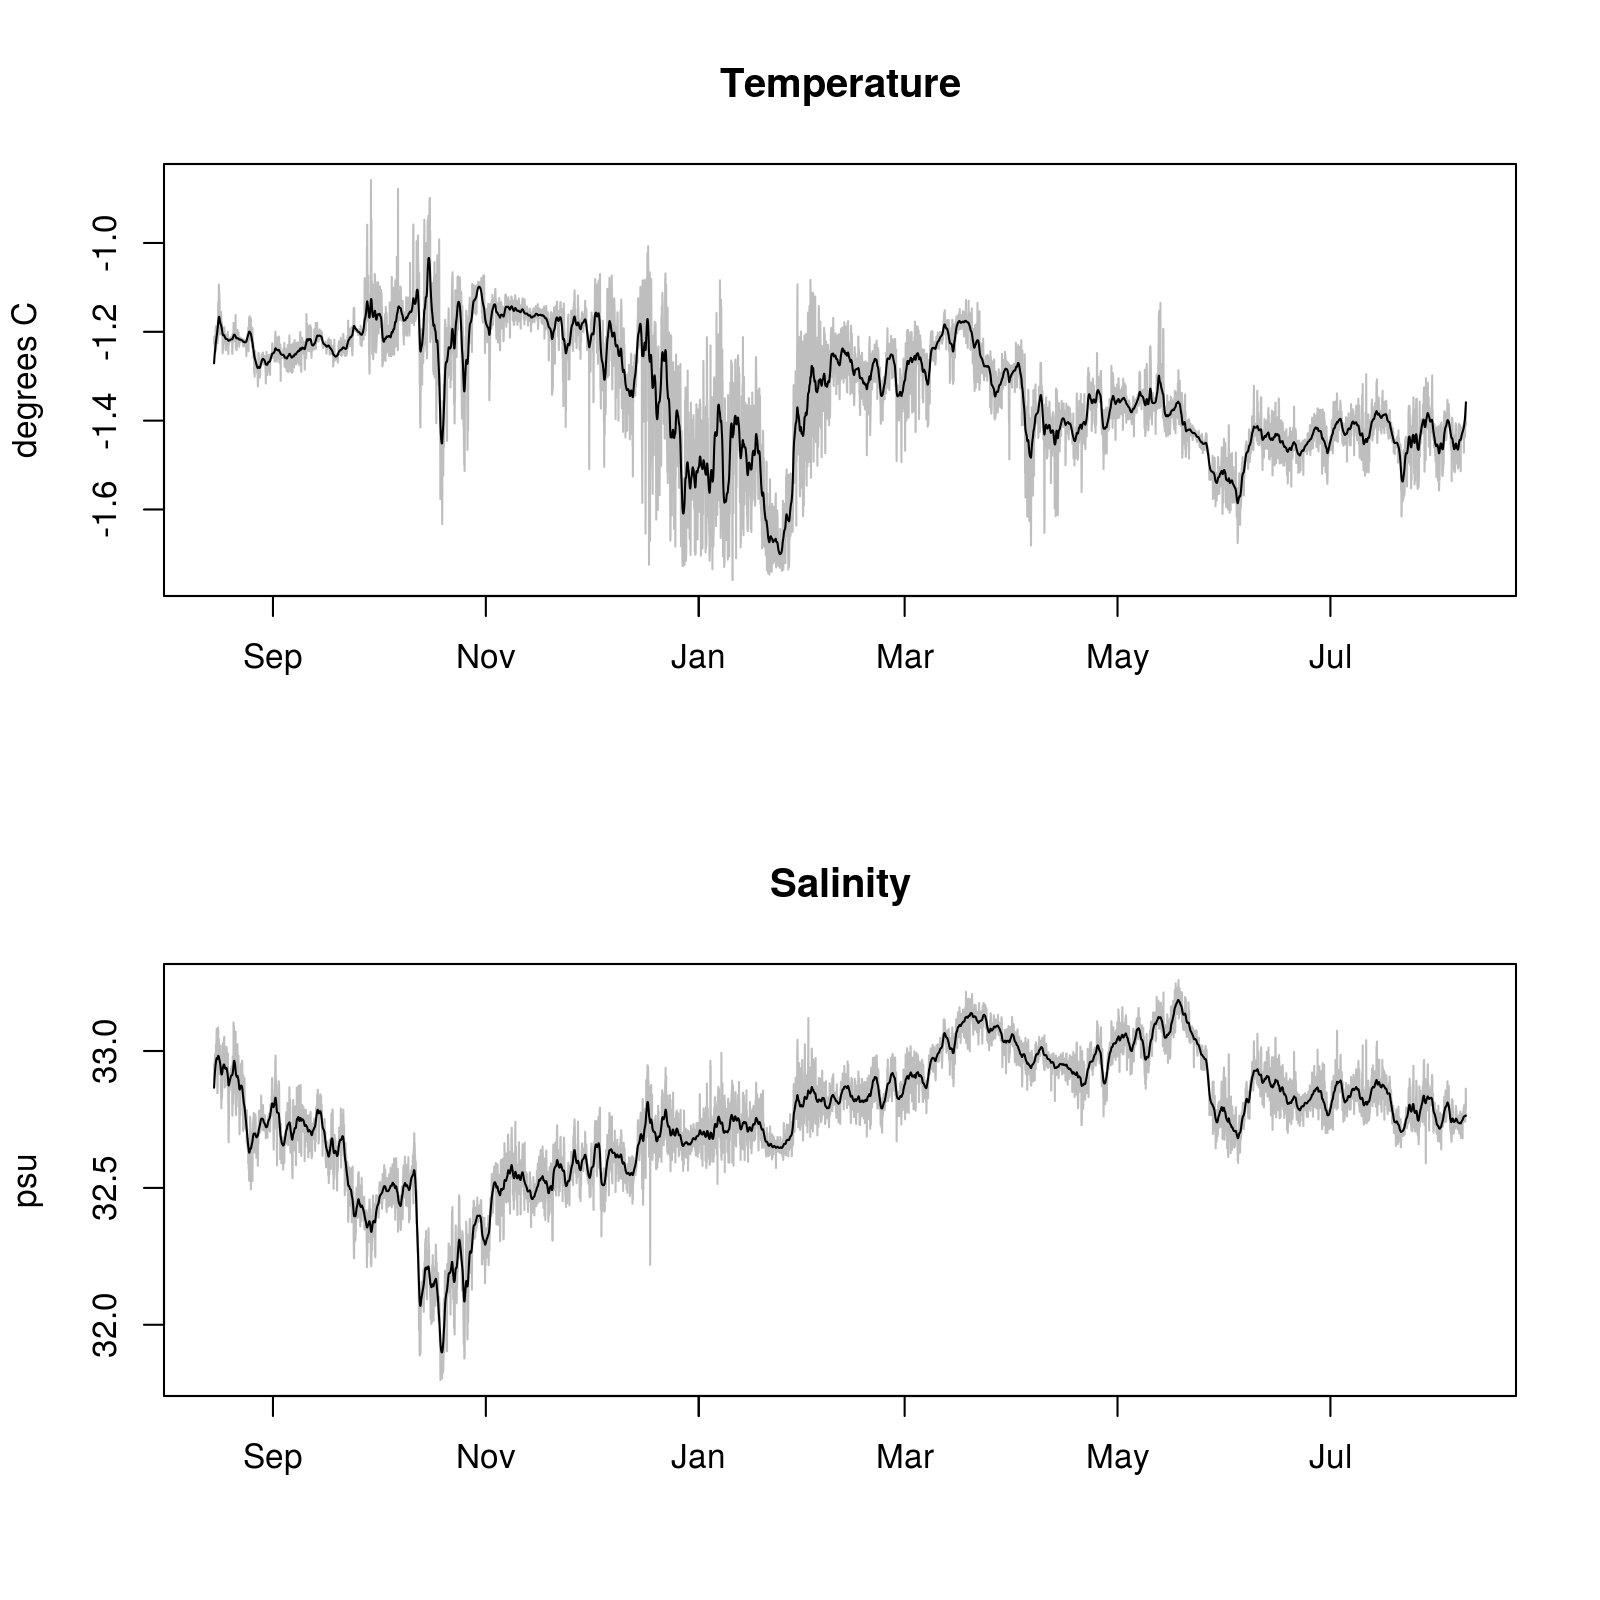
\includegraphics[width = 0.8\textwidth]{./figures/26_lpf_TS_81m_2013_2014.png}
\caption[Low-pass filtered T, S (81 m), 2013-2014]{Low-pass filtered T, S (81 m), August 2013 - August 2014}
\label{f:ctd_81_lpf_2013_2014}
\end{figure}

\begin{figure}  
\centering
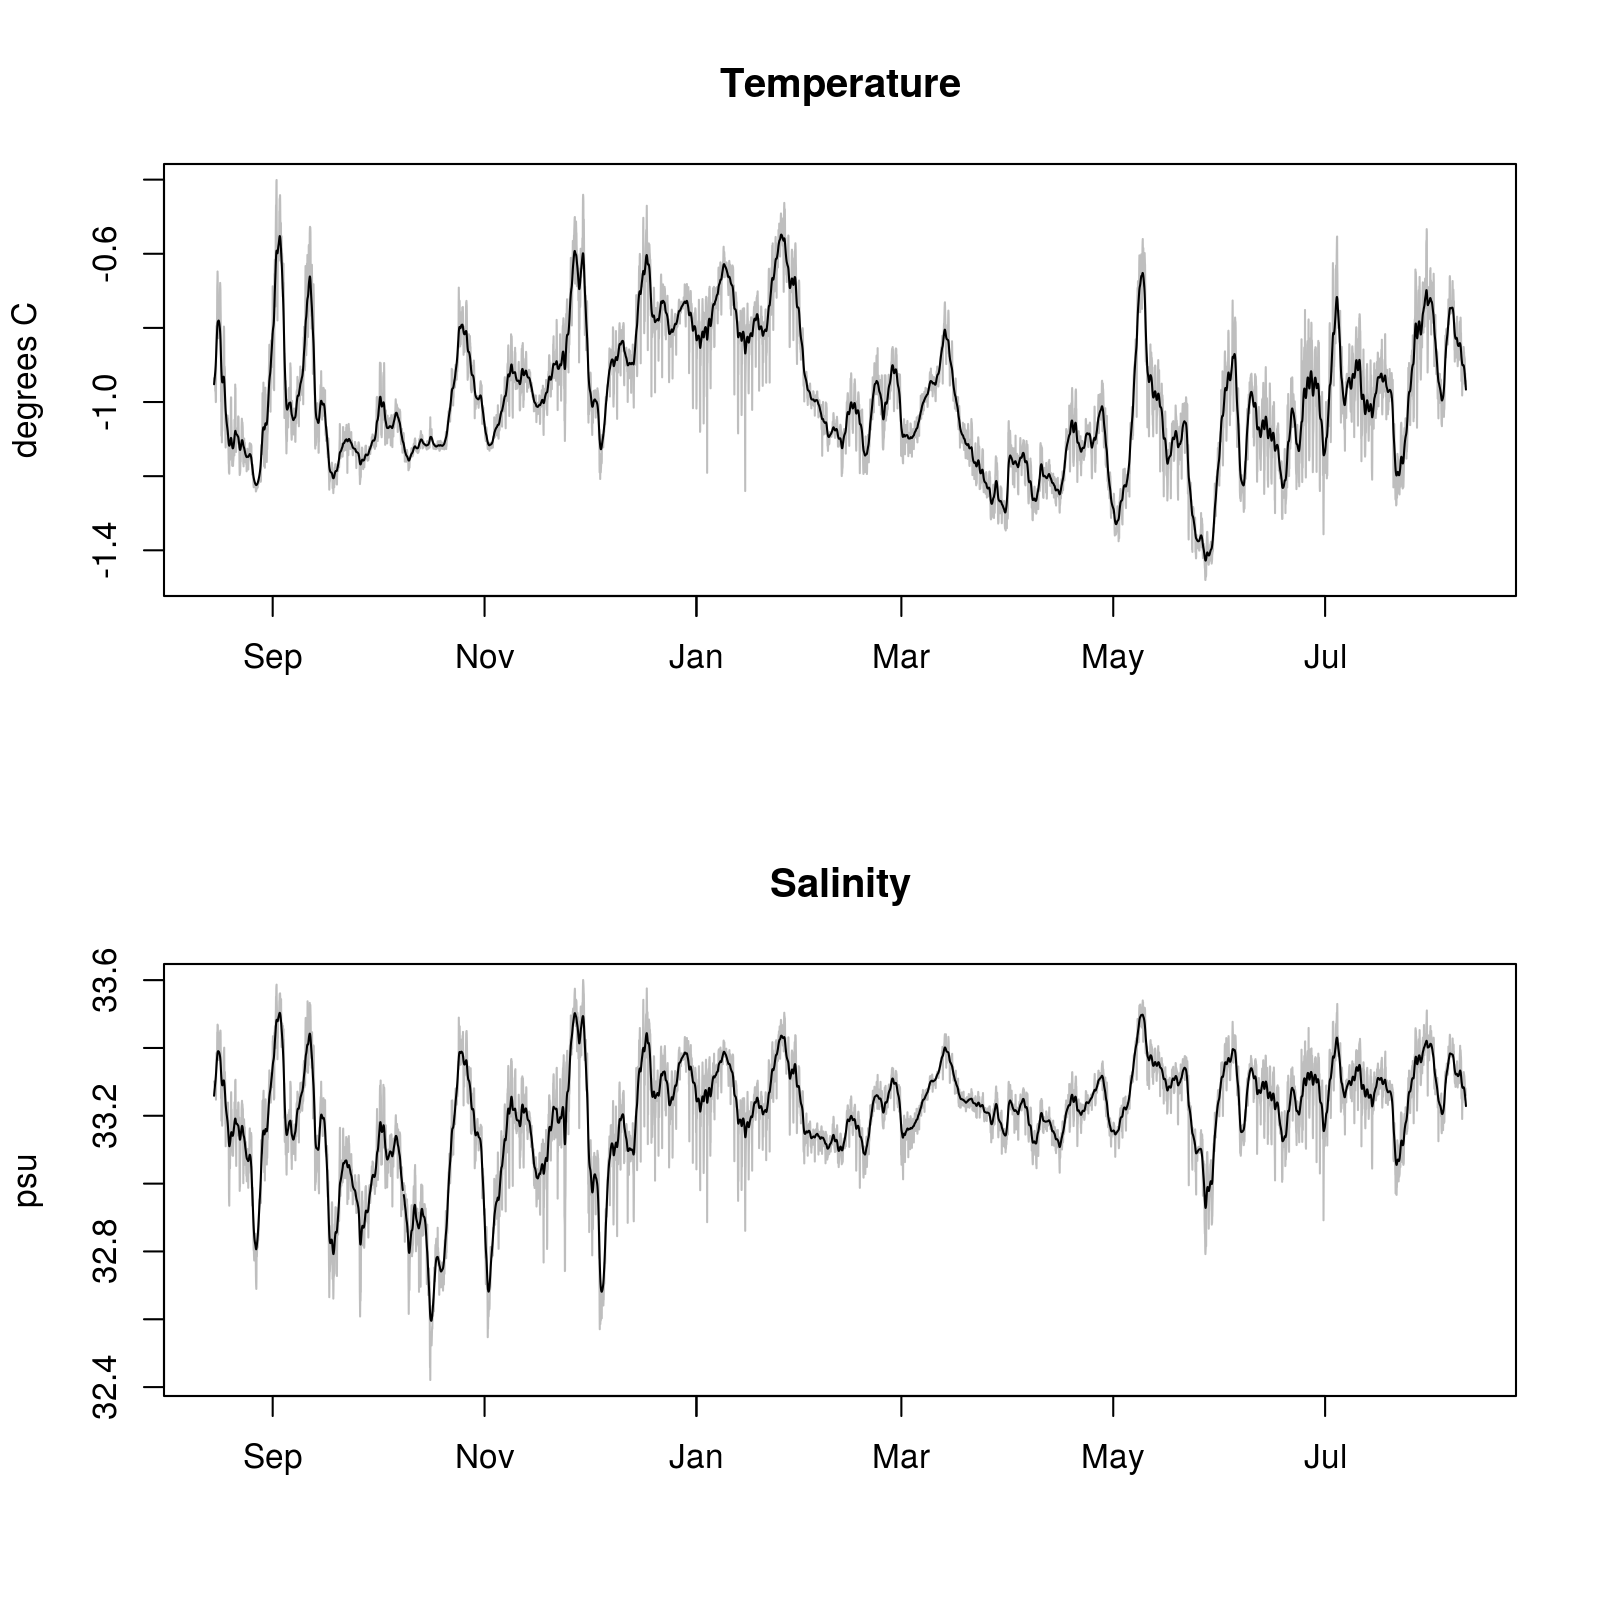
\includegraphics[width = 0.8\textwidth]{./figures/27_lpf_TS_155m_2013_2014.png}
\caption[Low-pass filtered T, S (155 m), 2013-2014]{Low-pass filtered T, S (155 m), August 2013 - August 2014}
\label{f:ctd_155_lpf_2013_2014}
\end{figure}


\begin{figure}  
\centering
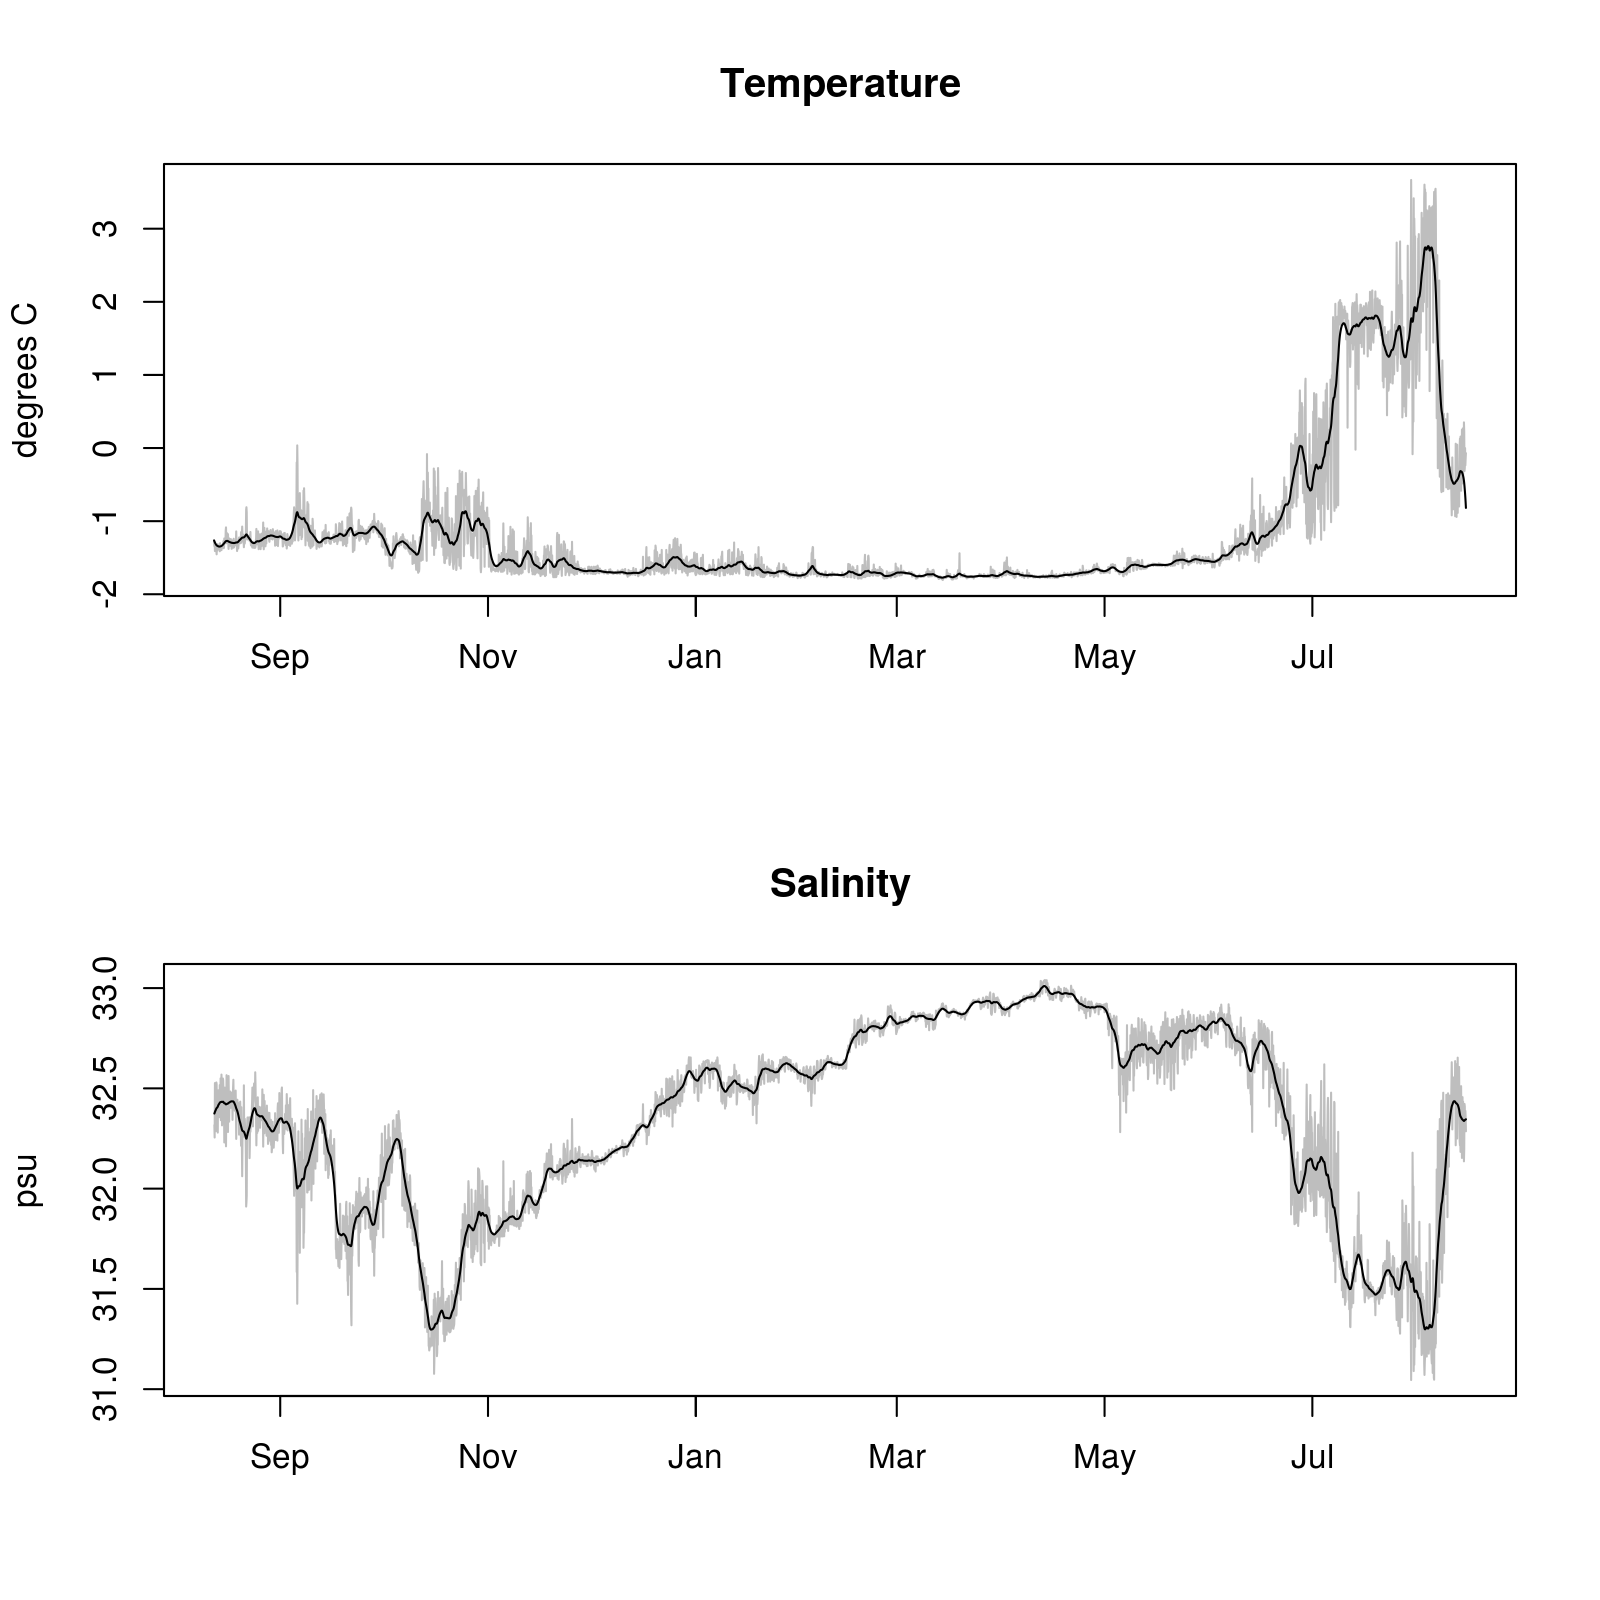
\includegraphics[width = 0.8\textwidth]{./figures/28_lpf_TS_35m_2014_2015.png}
\caption[Low-pass filtered T, S (35 m), 2014-2015]{Low-pass filtered T, S (35 m), August 2014 - August 2015}
\label{f:ctd_35_lpf_2014_2015}
\end{figure}

\begin{figure}  
\centering
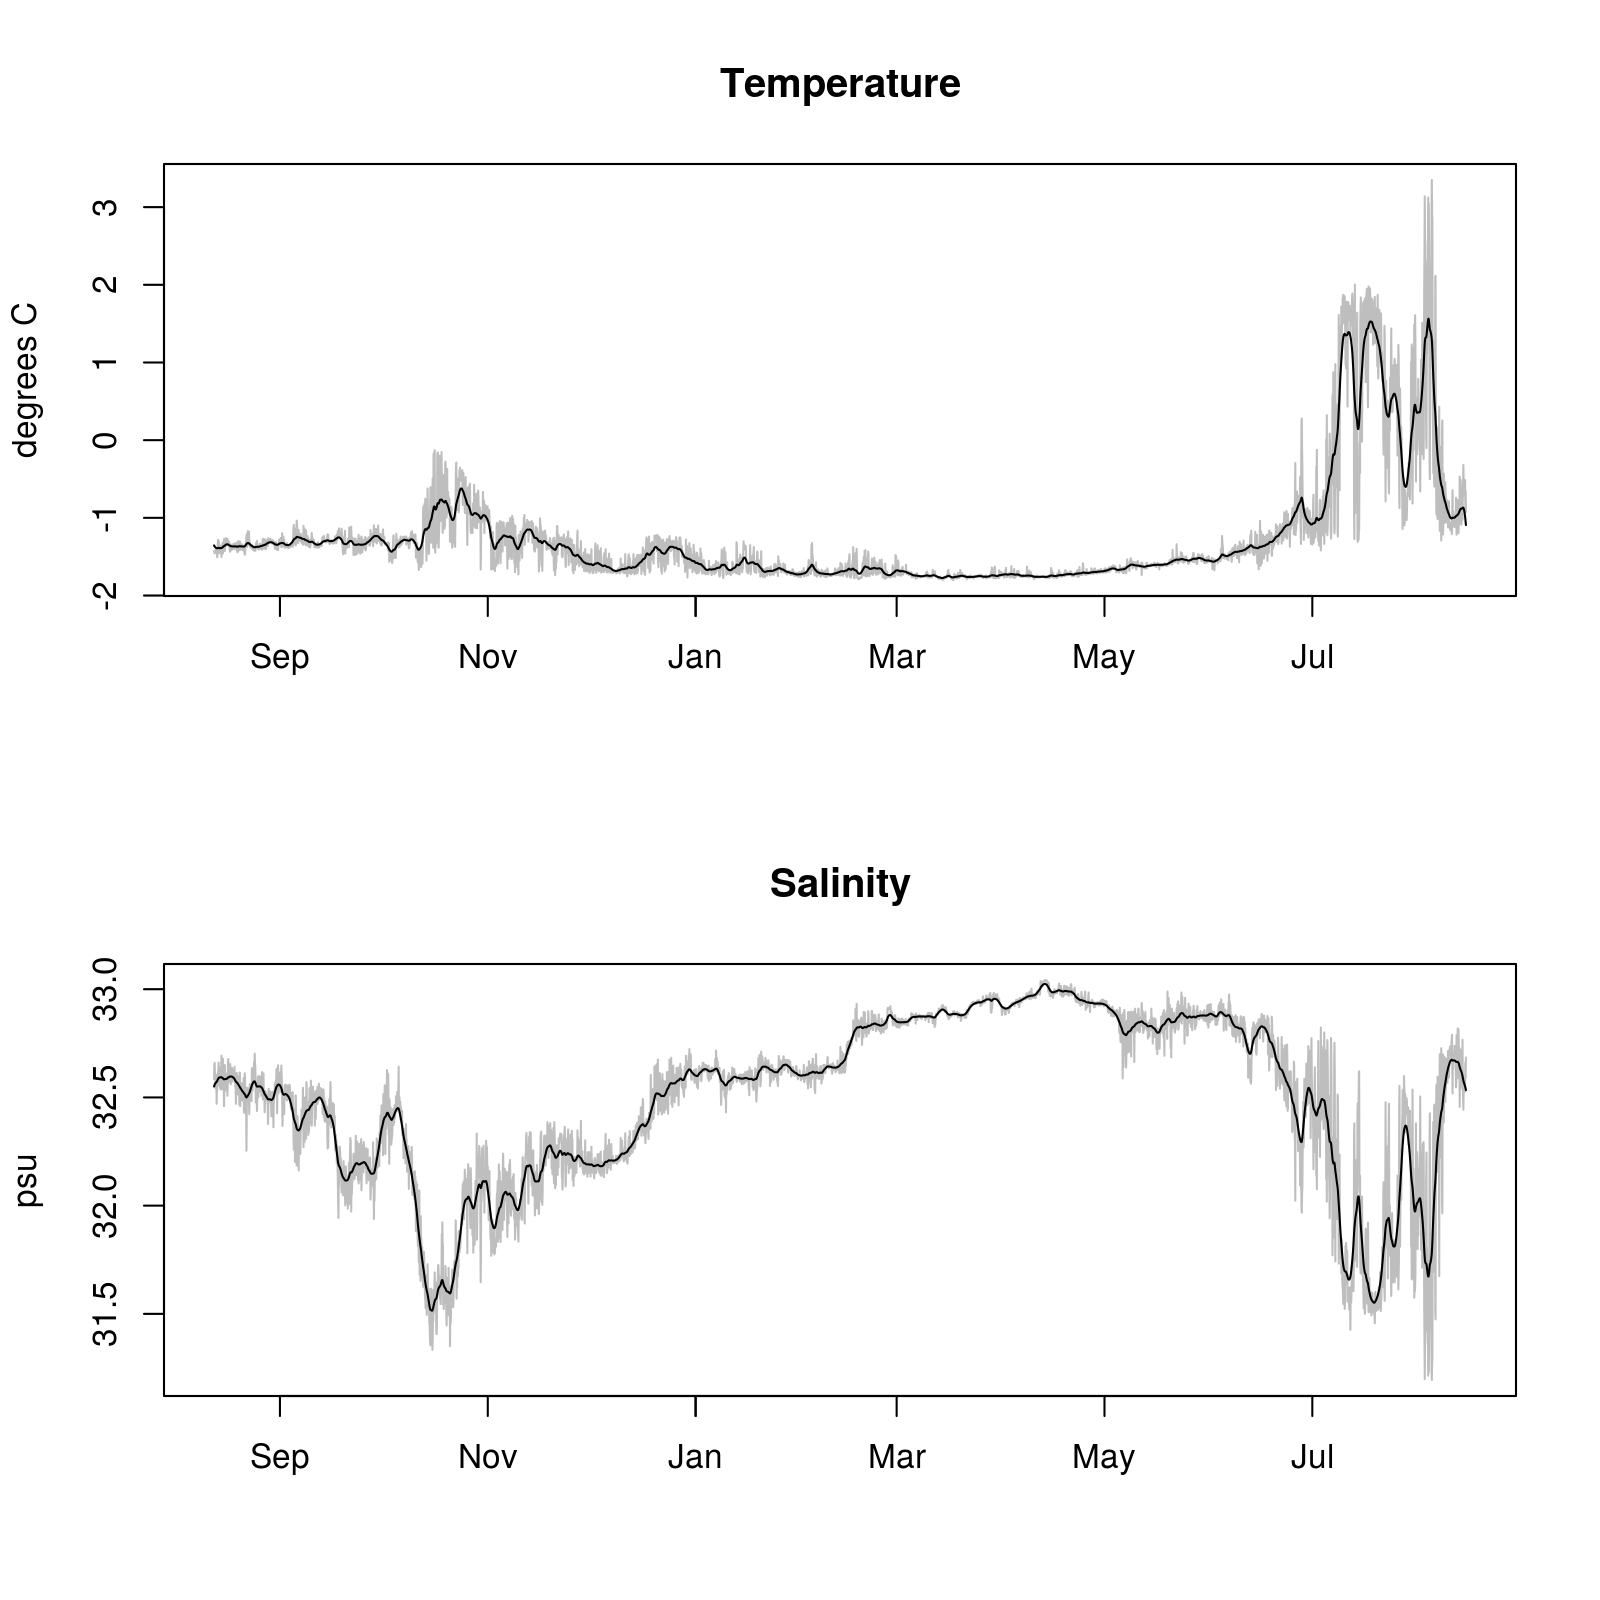
\includegraphics[width = 0.8\textwidth]{./figures/29_lpf_TS_47m_2014_2015.png}
\caption[Low-pass filtered T, S (47 m), 2014-2015]{Low-pass filtered T, S (47 m), August 2014 - August 2015}
\label{f:ctd_47_lpf_2014_2015}
\end{figure}

\begin{figure}  
\centering
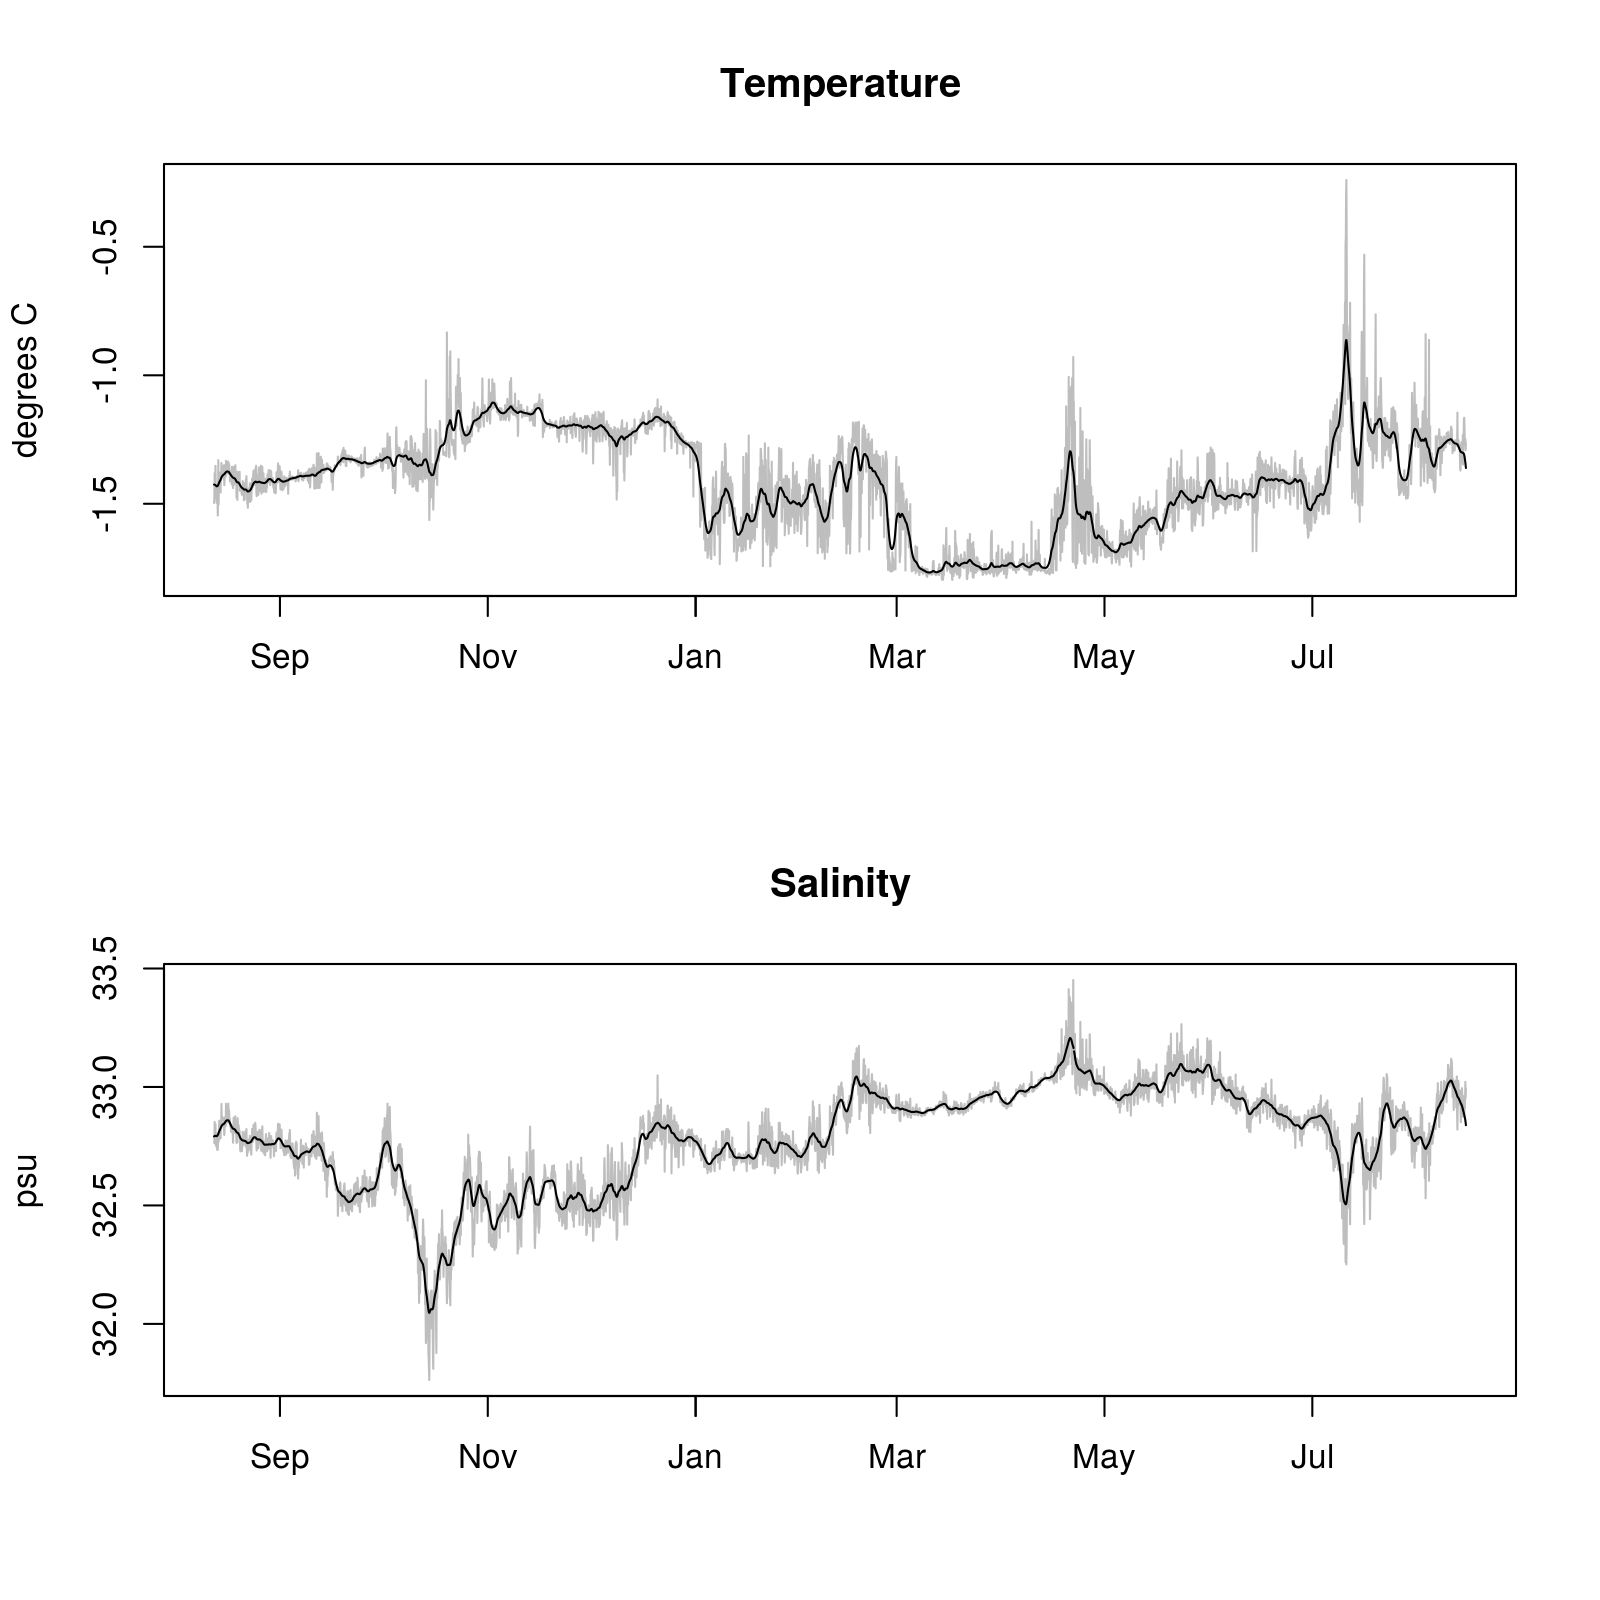
\includegraphics[width = 0.8\textwidth]{./figures/30_lpf_TS_81m_2014_2015.png}
\caption[Low-pass filtered T, S (81 m), 2014-2015]{Low-pass filtered T, S (81 m), August 2014 - August 2015}
\label{f:ctd_81_lpf_2014_2015}
\end{figure}

\begin{figure}  
\centering
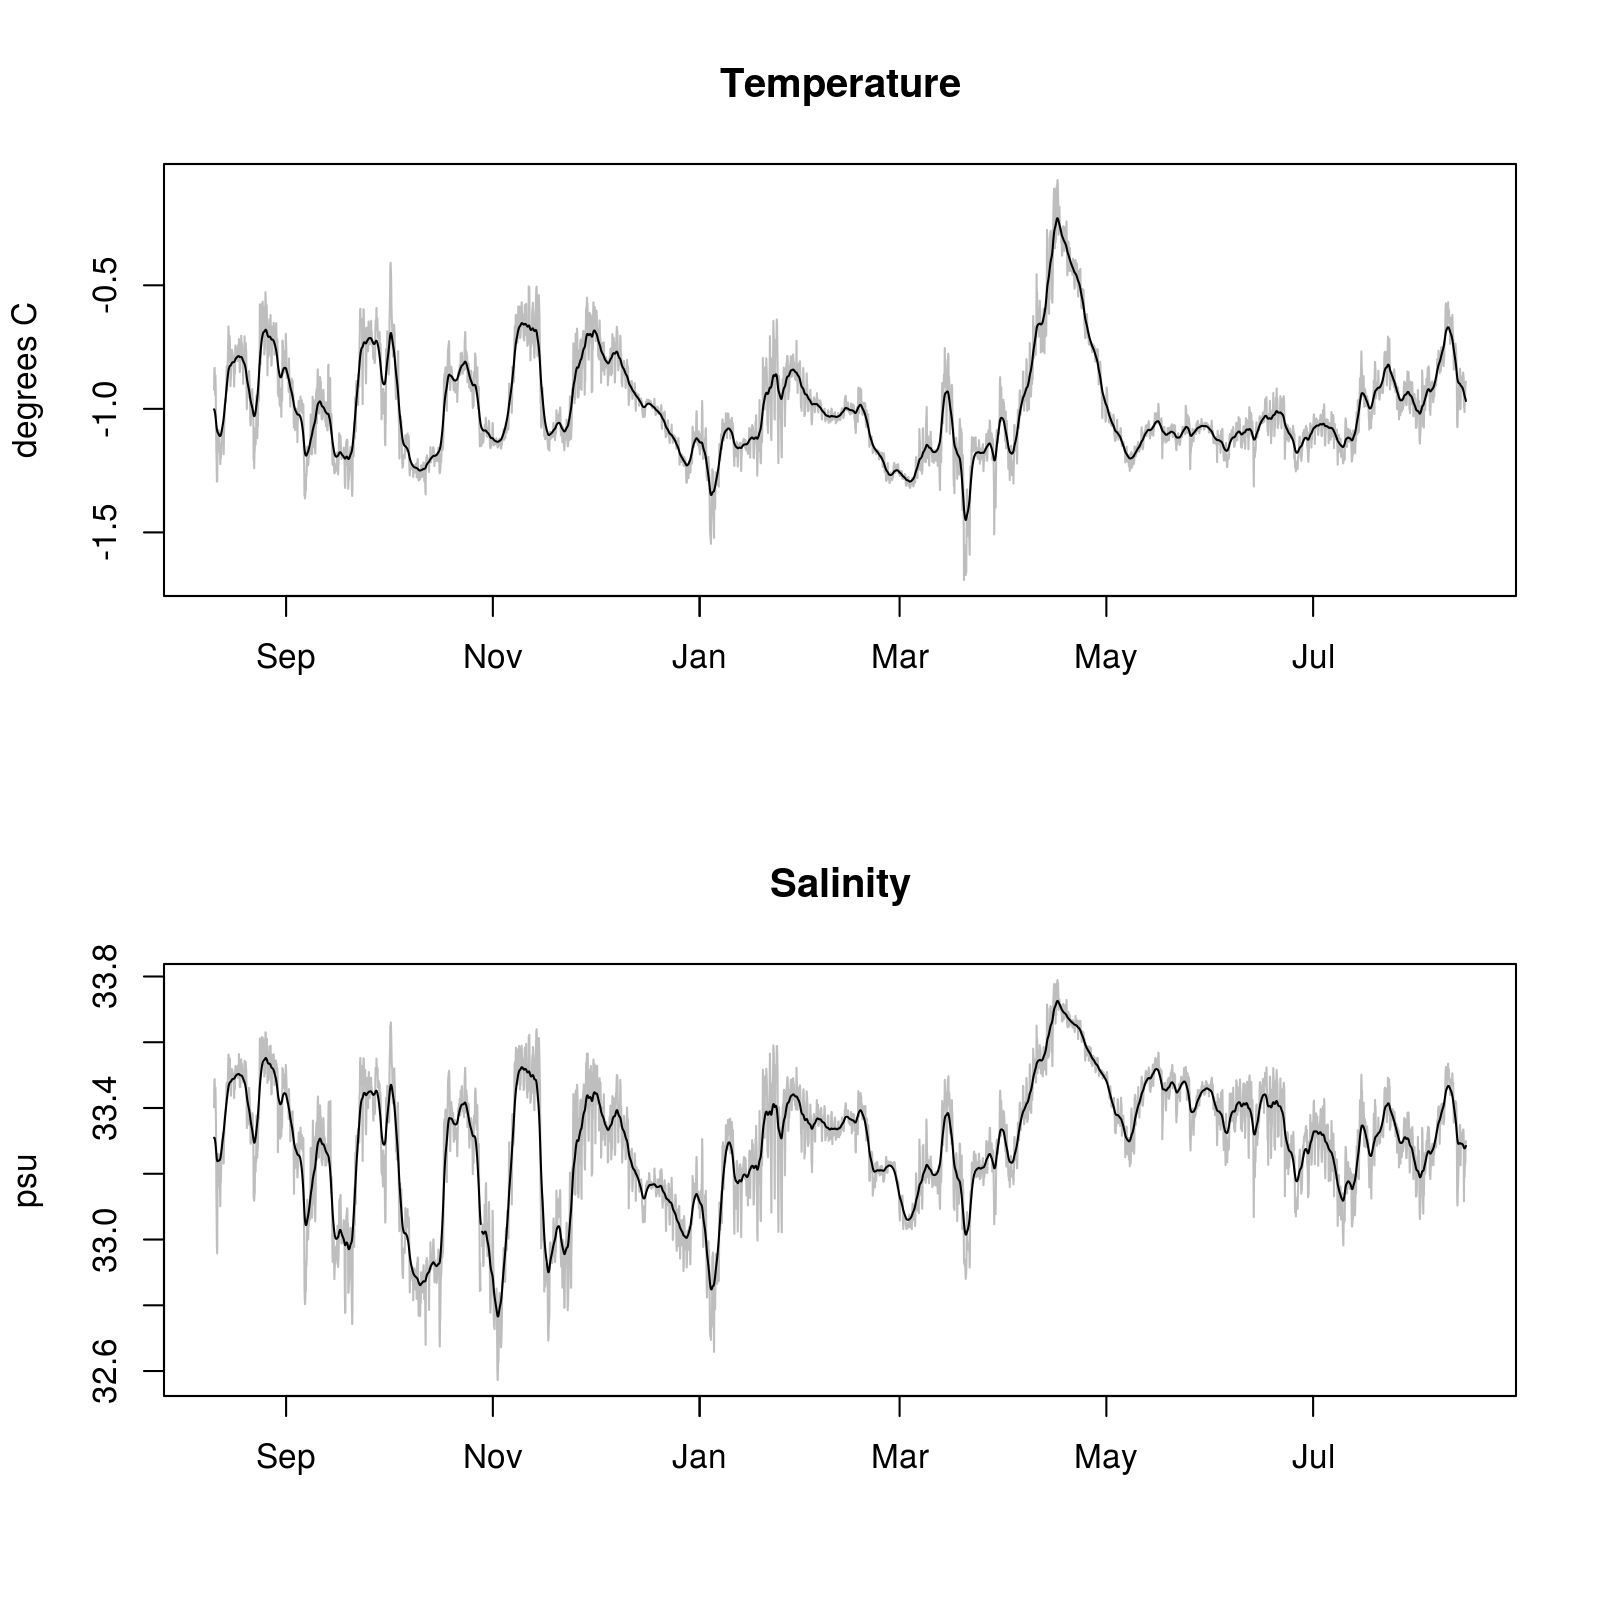
\includegraphics[width = 0.8\textwidth]{./figures/31_lpf_TS_155m_2014_2015.png}
\caption[Low-pass filtered T, S (155 m), 2014-2015]{Low-pass filtered T, S (155 m), August 2014 - August 2015}
\label{f:ctd_155_lpf_2014_2015}
\end{figure}


\begin{figure}  
\centering
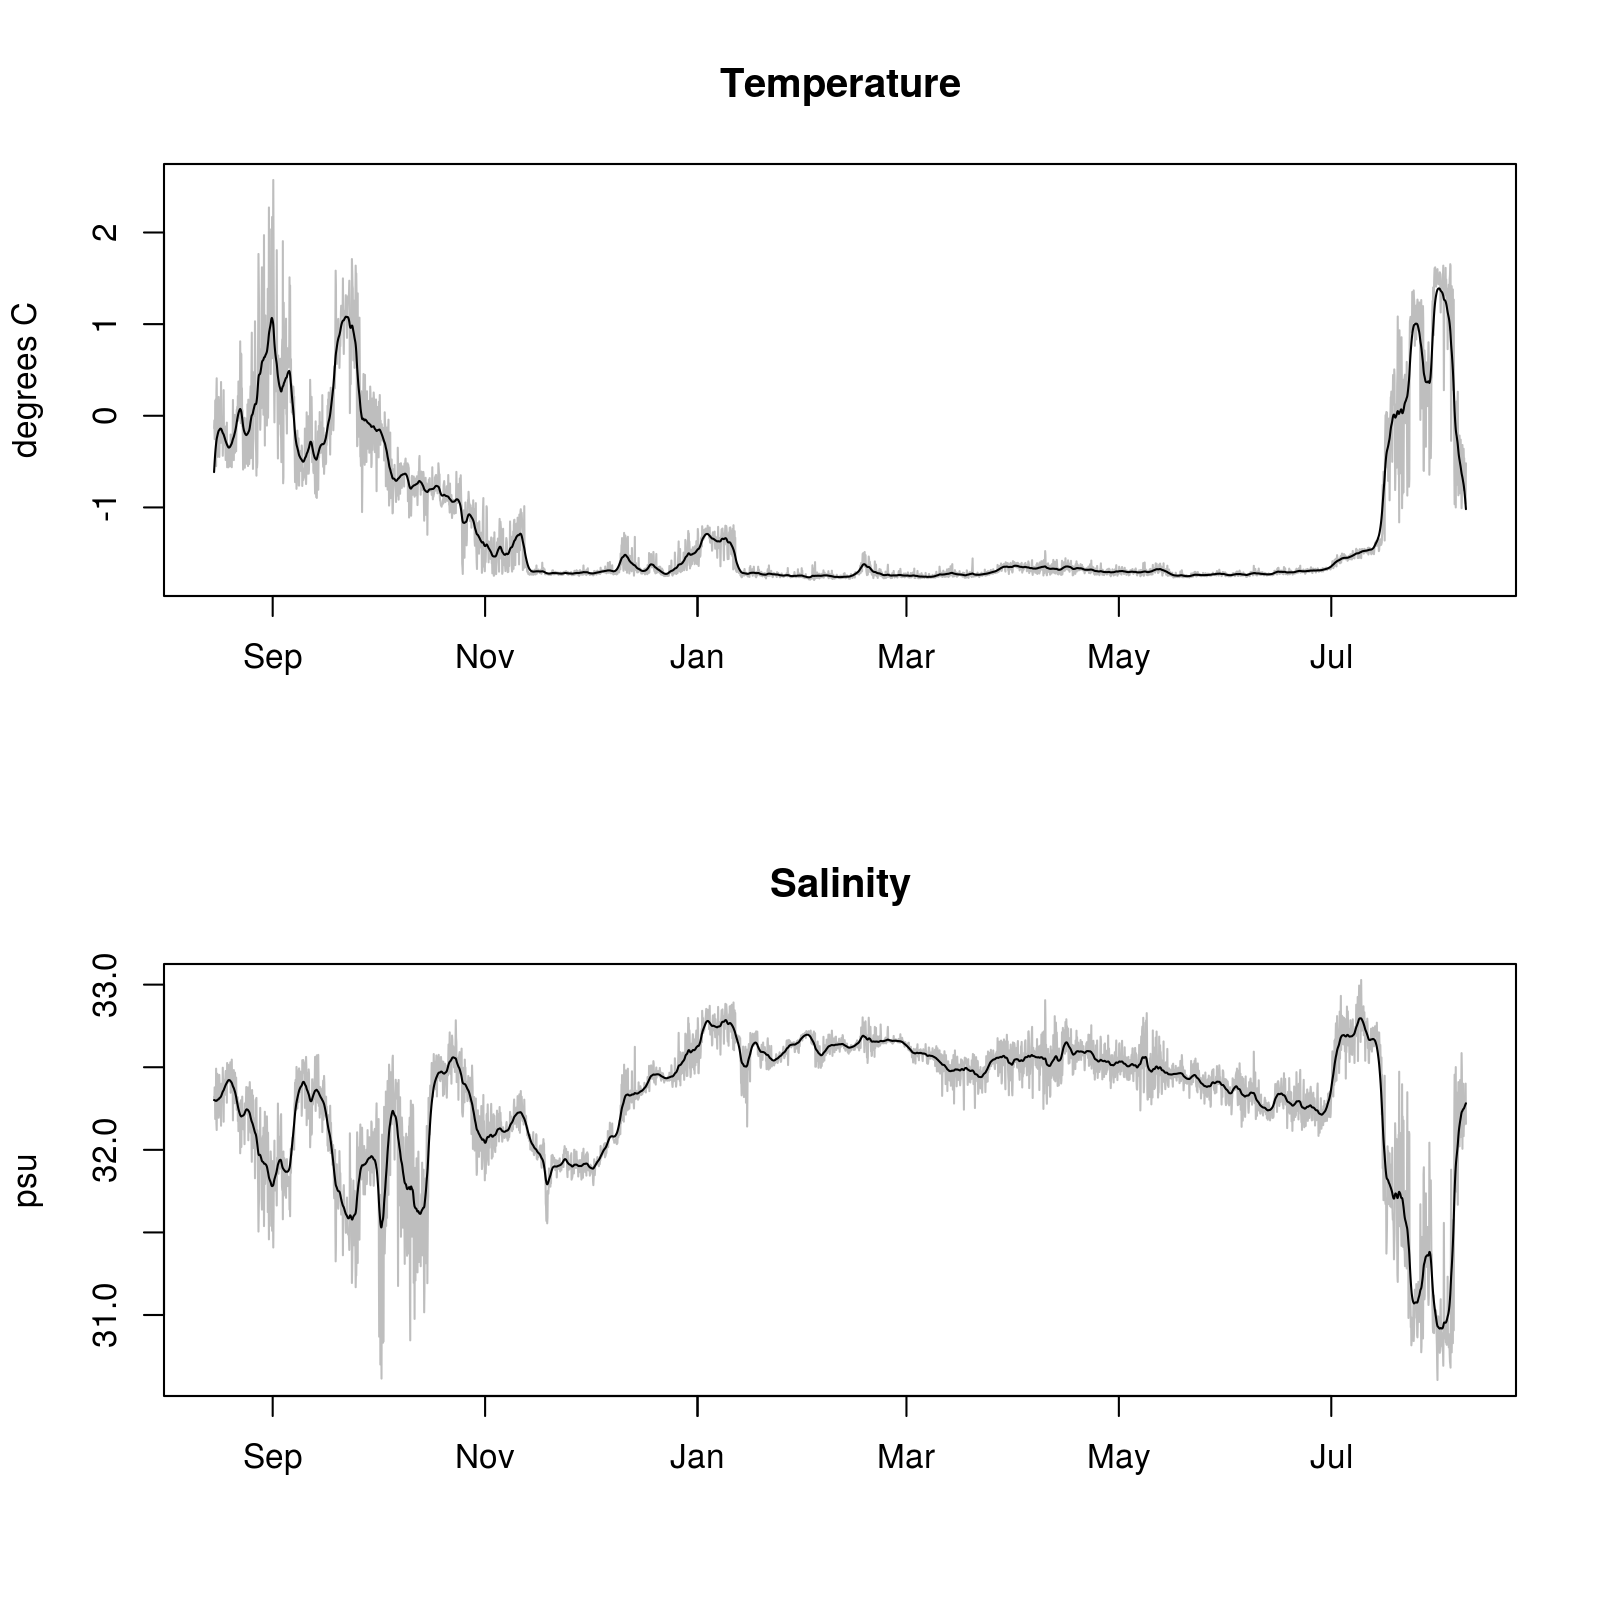
\includegraphics[width = 0.8\textwidth]{./figures/32_lpf_TS_35m_2015_2016.png}
\caption[Low-pass filtered T, S (35 m), 2015-2016]{Low-pass filtered T, S (35 m), August 2015 - August 2016}
\label{f:ctd_35_lpf_2015_2016}
\end{figure}

\begin{figure}  
\centering
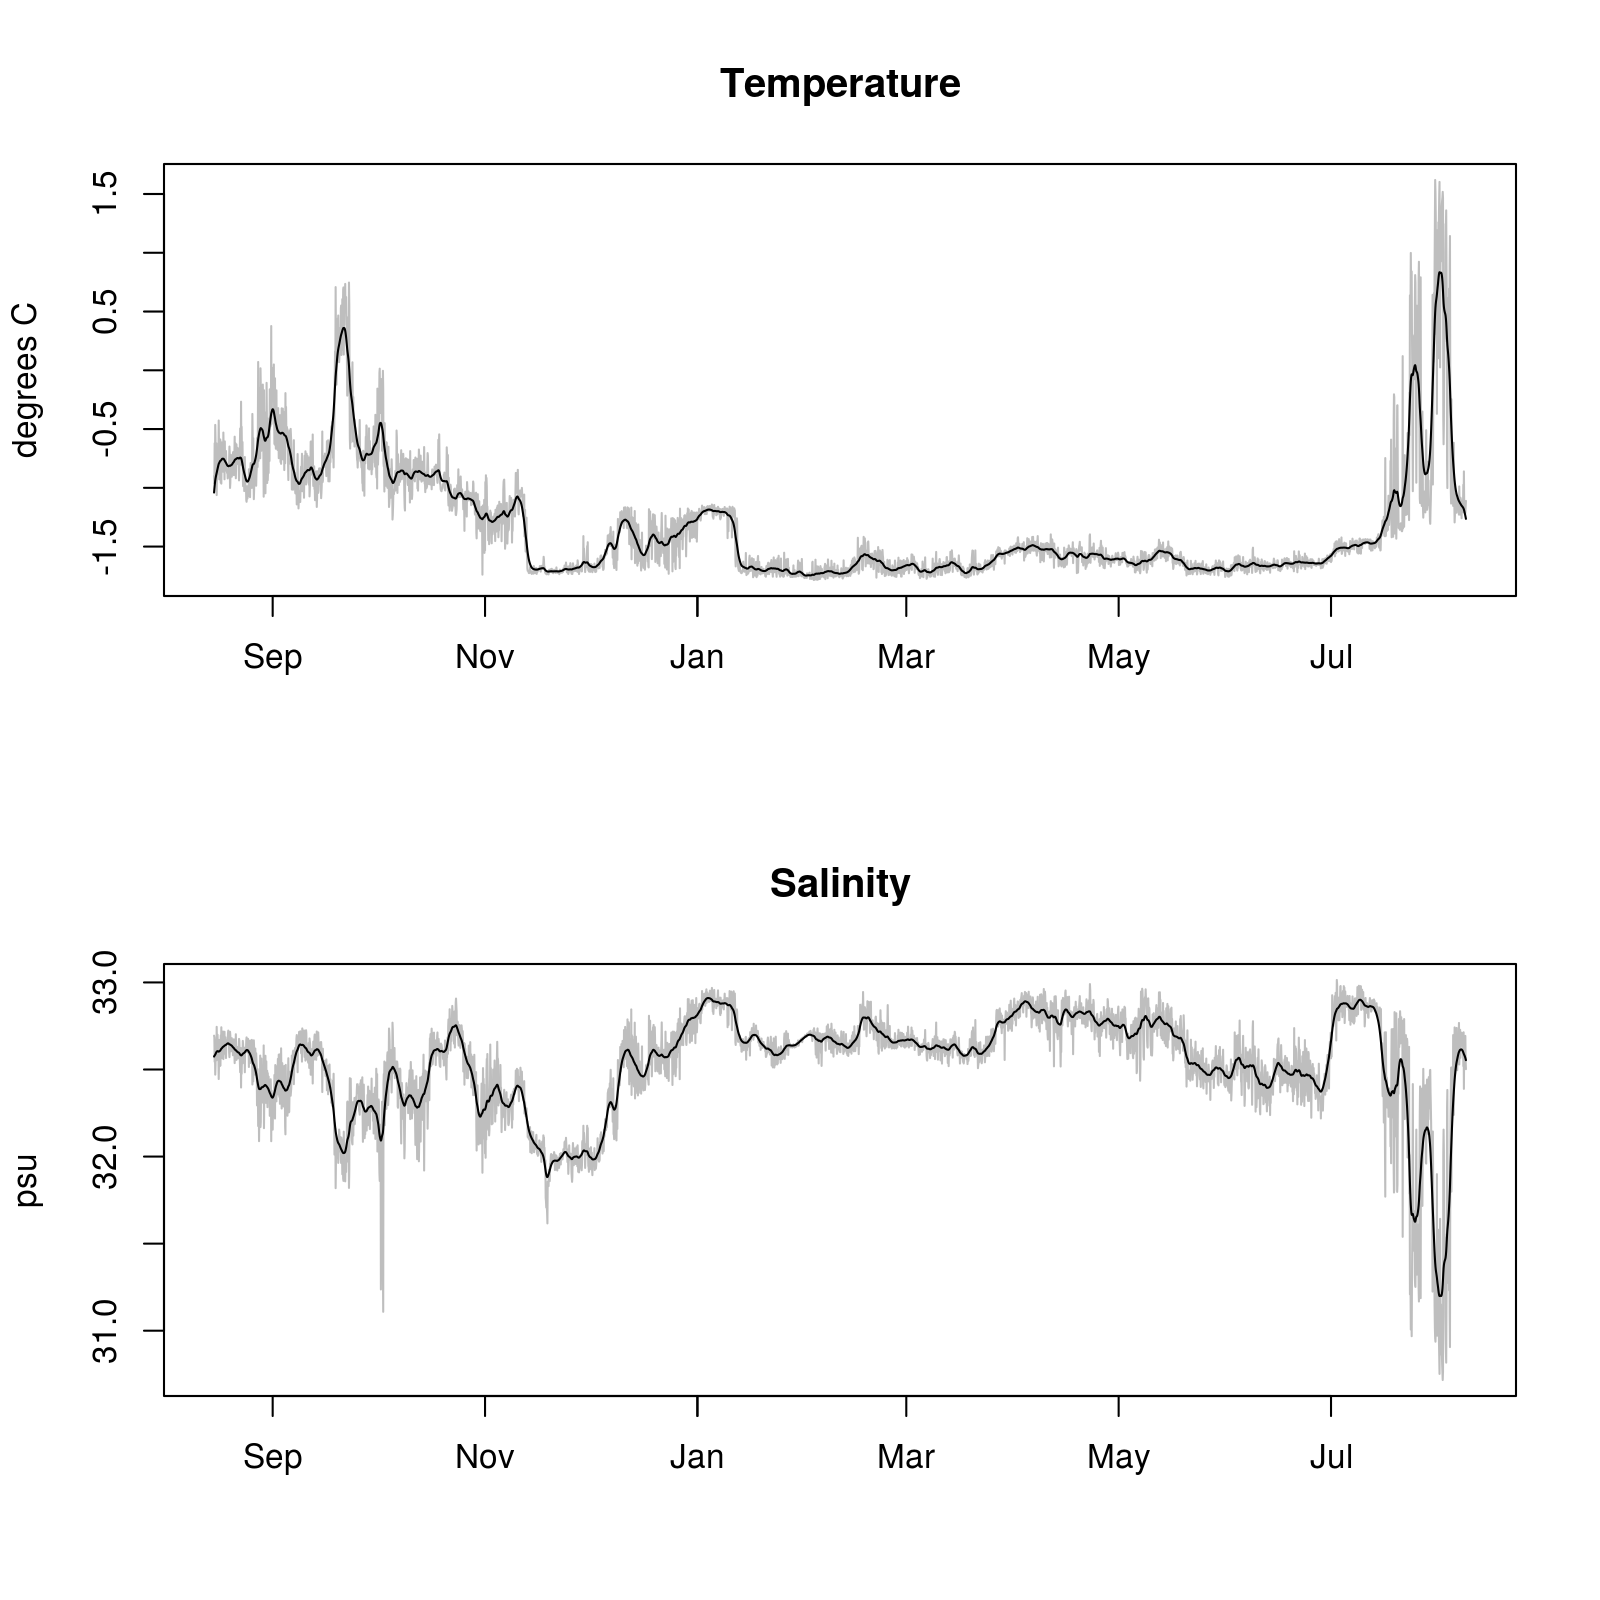
\includegraphics[width = 0.8\textwidth]{./figures/33_lpf_TS_47m_2015_2016.png}
\caption[Low-pass filtered T, S (47 m), 2015-2016]{Low-pass filtered T, S (47 m), August 2015 - August 2016}
\label{f:ctd_47_lpf_2015_2016}
\end{figure}

\begin{figure}  
\centering
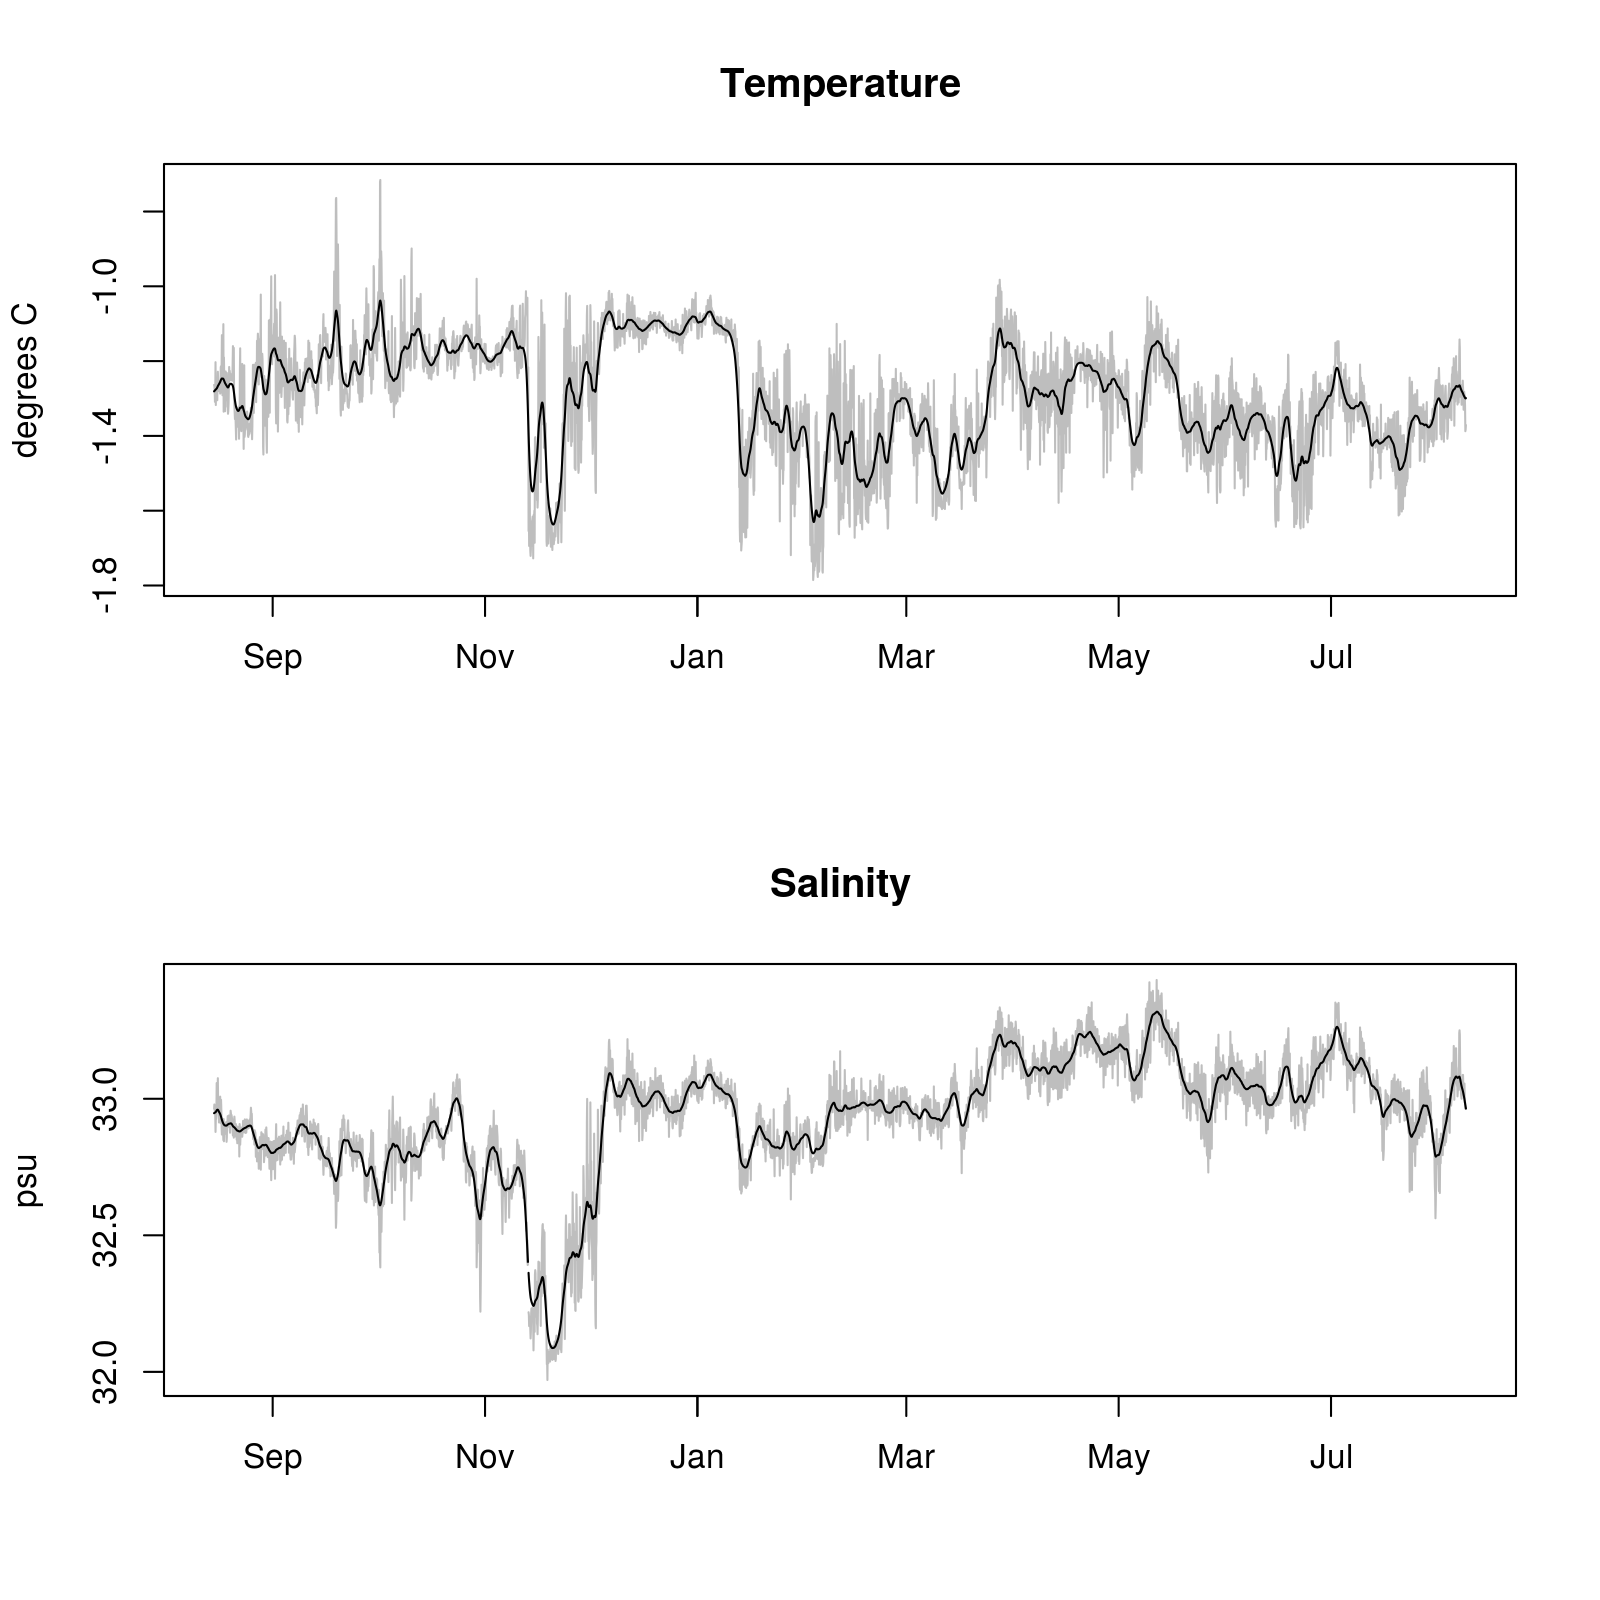
\includegraphics[width = 0.8\textwidth]{./figures/34_lpf_TS_81m_2015_2016.png}
\caption[Low-pass filtered T, S (81 m), 2015-2016]{Low-pass filtered T, S (81 m), August 2015 - August 2016}
\label{f:ctd_81_lpf_2015_2016}
\end{figure}

\begin{figure}  
\centering
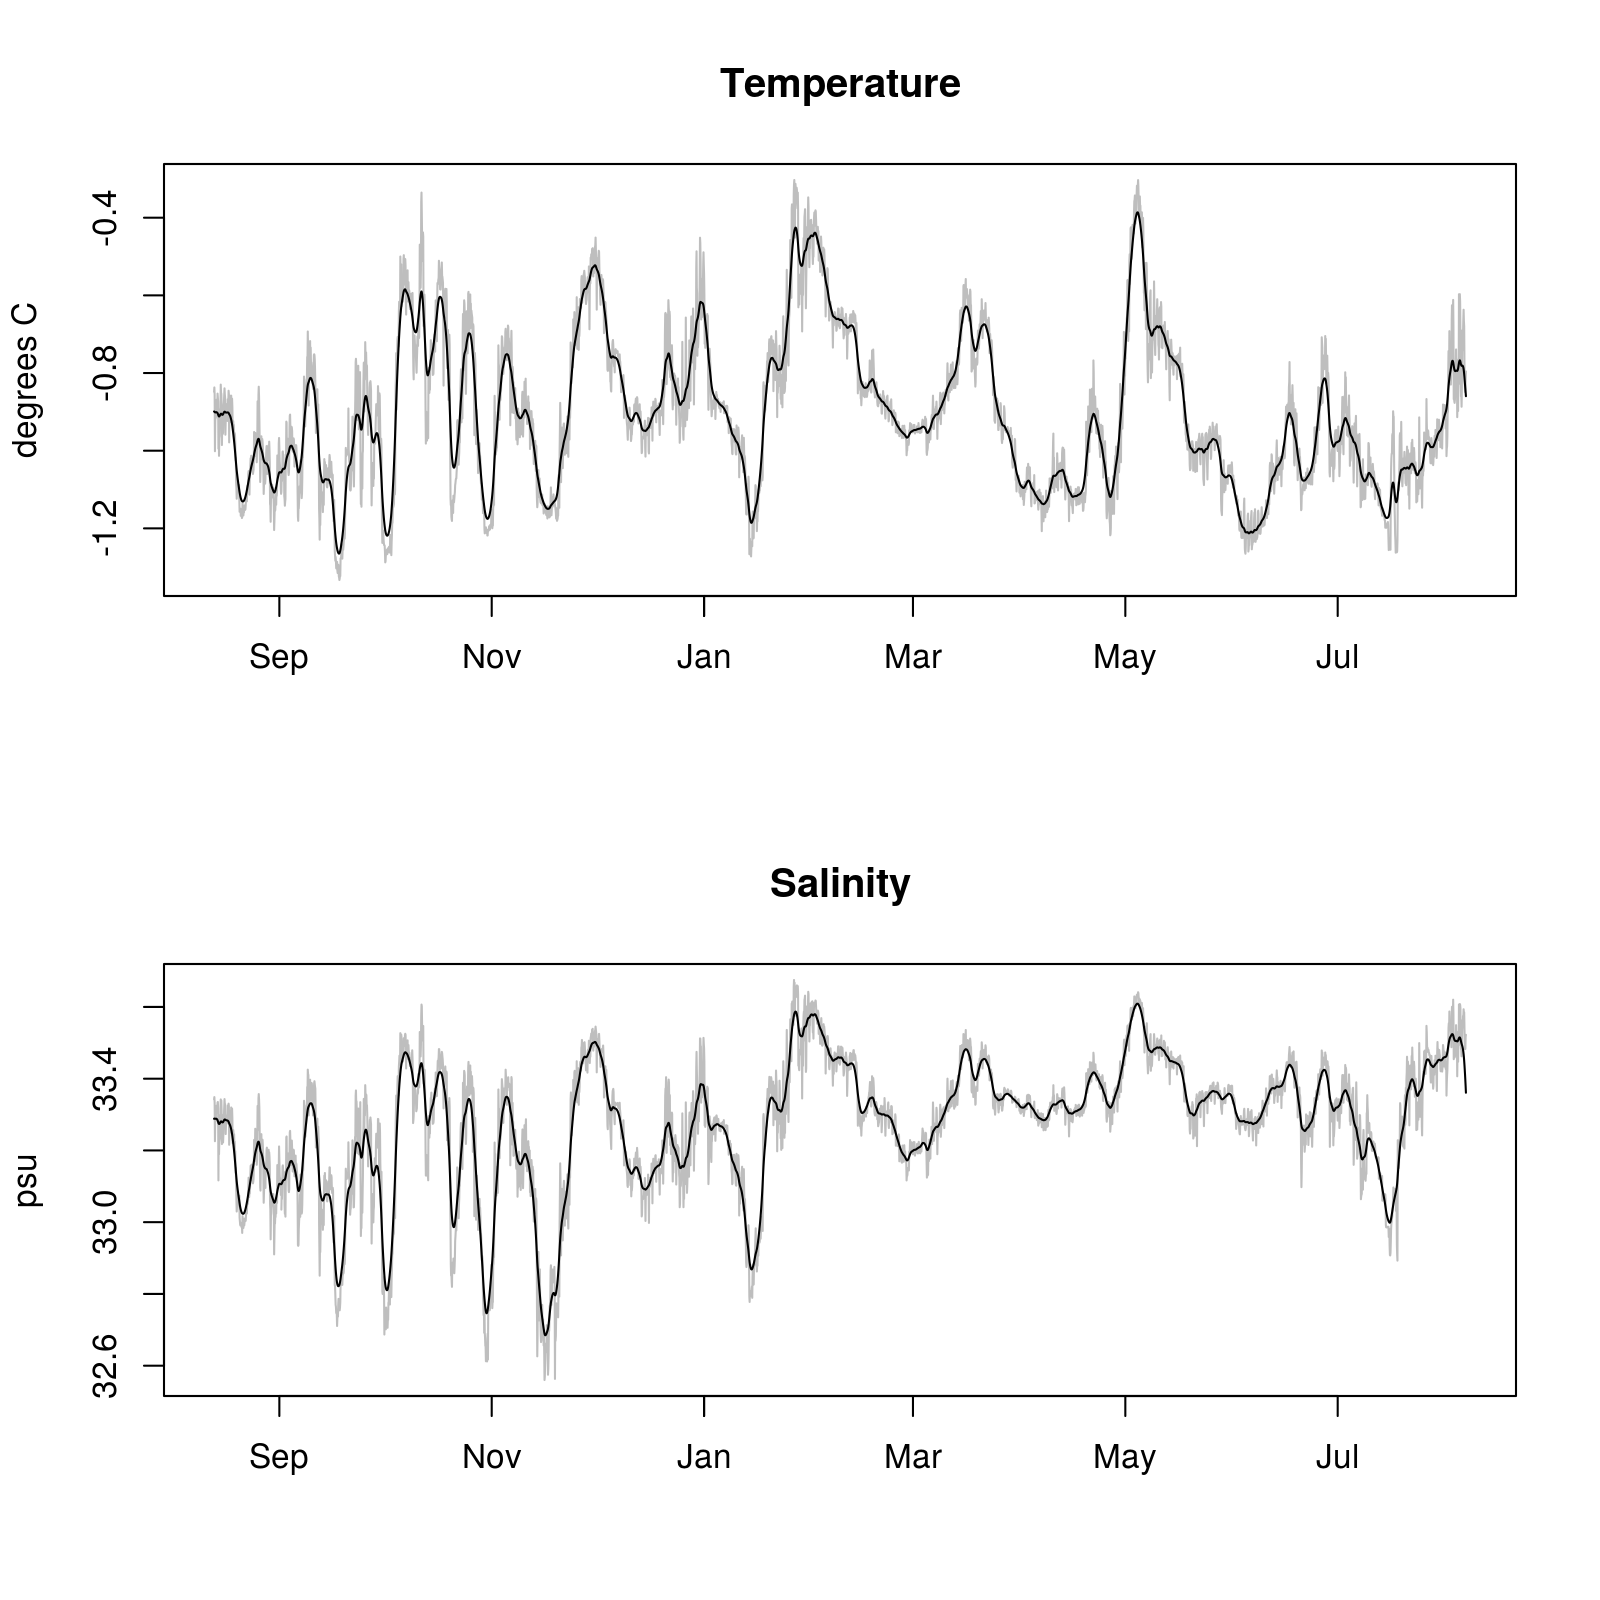
\includegraphics[width = 0.8\textwidth]{./figures/35_lpf_TS_155m_2015_2016.png}
\caption[Low-pass filtered T, S (155 m), 2015-2016]{Low-pass filtered T, S (155 m), August 2015 - August 2016}
\label{f:ctd_155_lpf_2015_2016}
\end{figure}

\pagebreak
\newpage

\begin{figure}  
\centering
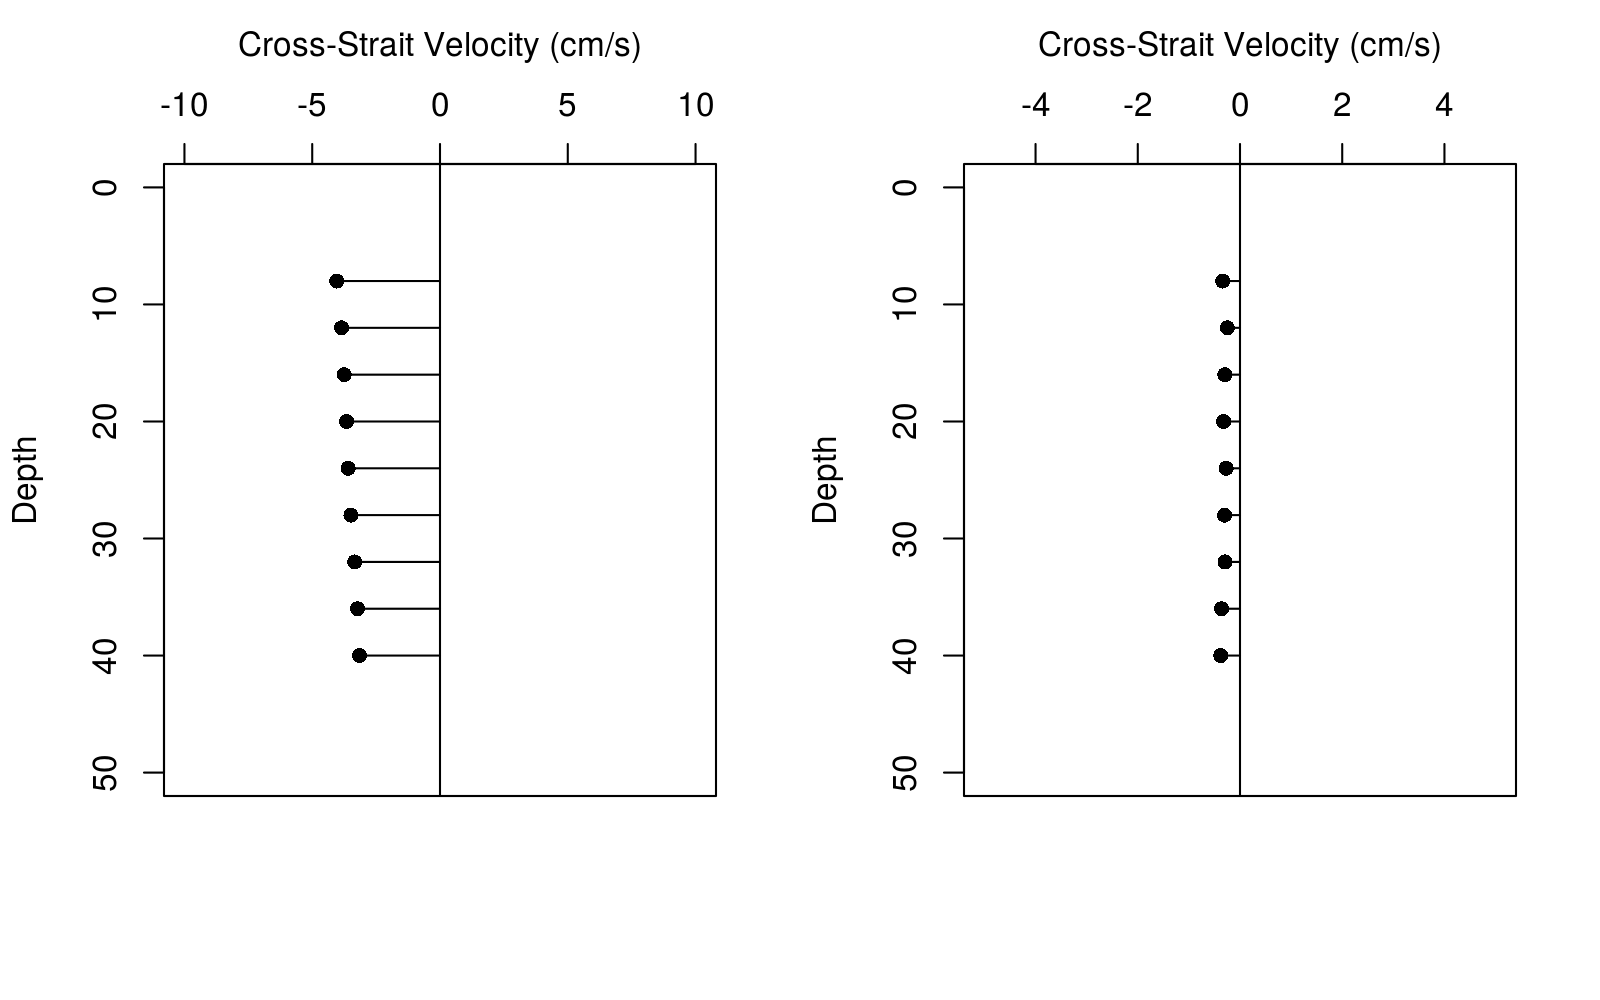
\includegraphics[width = 0.8\textwidth]{./figures/36_amf_2014_2015.png}
\caption[Mean flow, 2014-2015]{Mean flow, August 2014 - August 2015}
\label{f:amf_2014_2015}
\end{figure}

\begin{figure}  
\centering
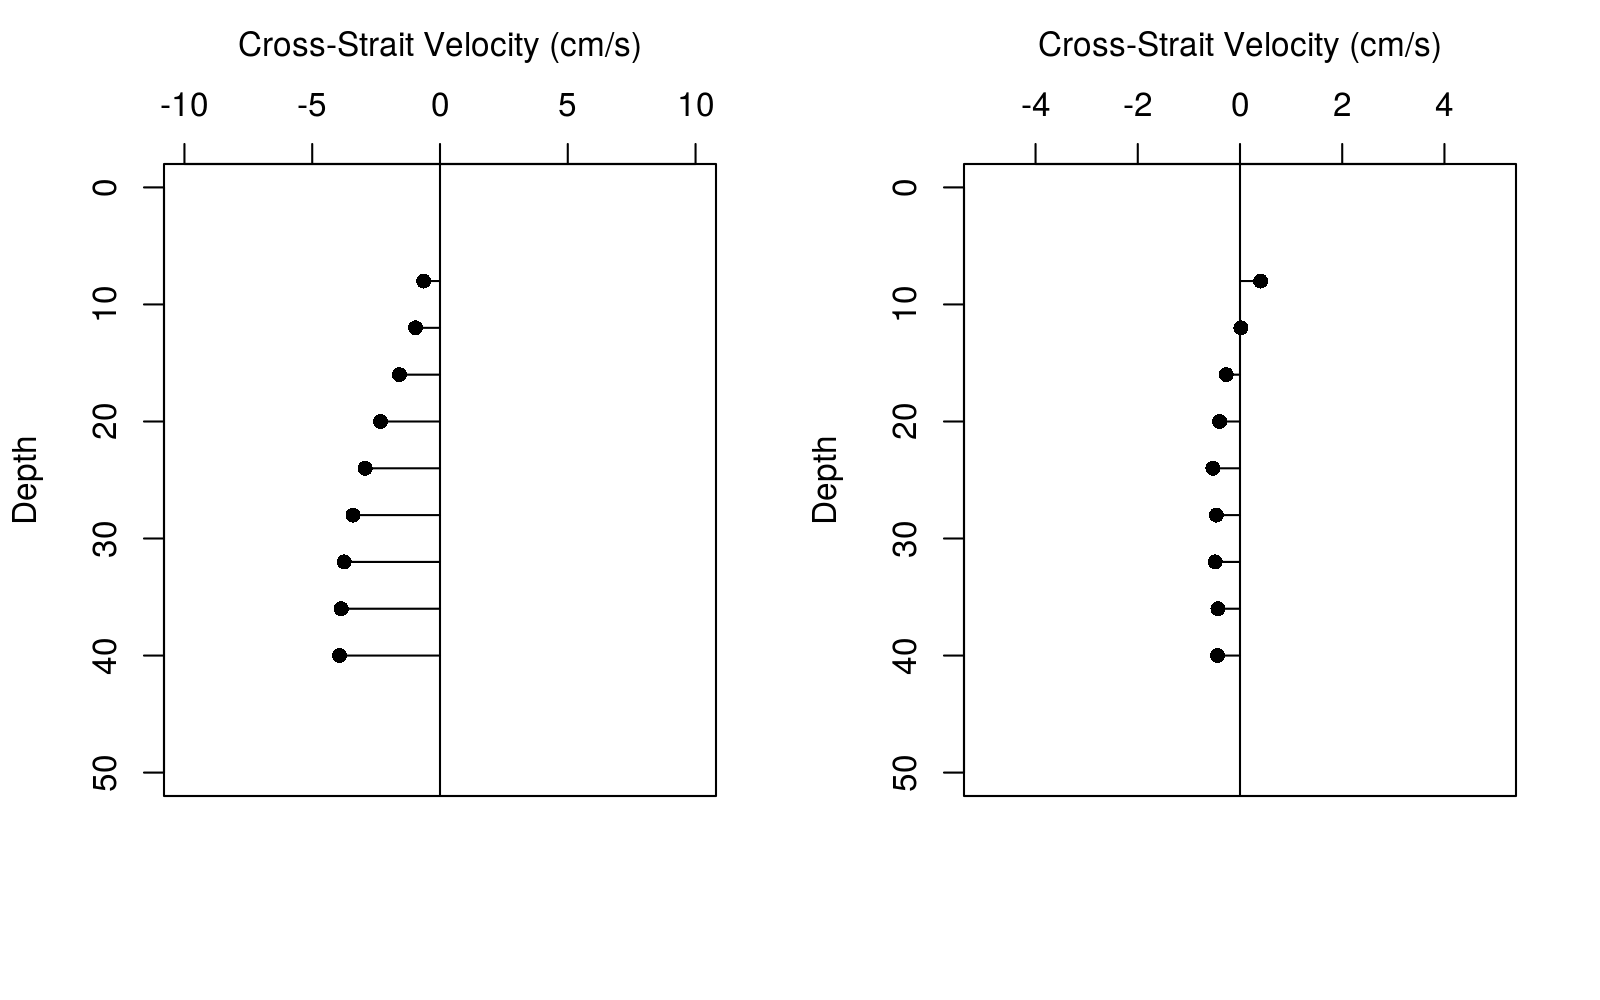
\includegraphics[width = 0.8\textwidth]{./figures/37_amf_2015_2016.png}
\caption[Mean flow, 2015-2016]{Mean flow,, August 2015 - August 2016}
\label{f:amf_2015_2016}
\end{figure}


\begin{figure}  
\centering
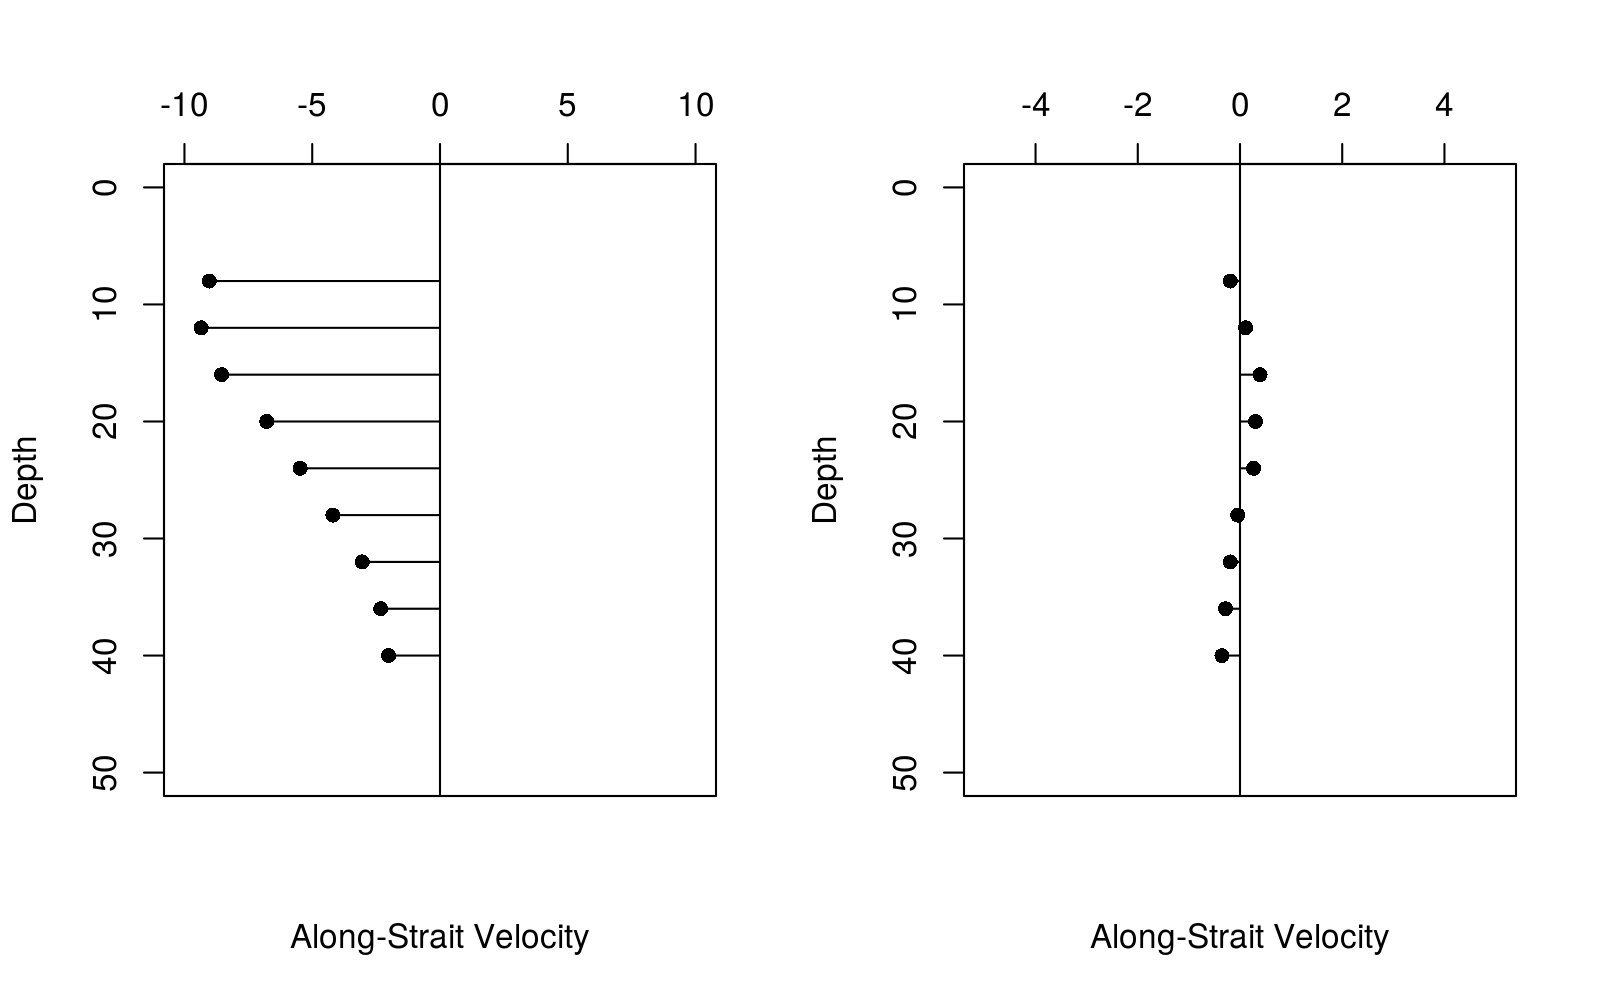
\includegraphics[width = 0.8\textwidth]{./figures/38_smf_lateSummer_2014.png}
\caption[Mean flow, Late Summer, 2014]{Mean flow, Late Summer: August 2014 to September 2014}
\label{f:smf_ls_2014}
\end{figure}

\begin{figure}  
\centering
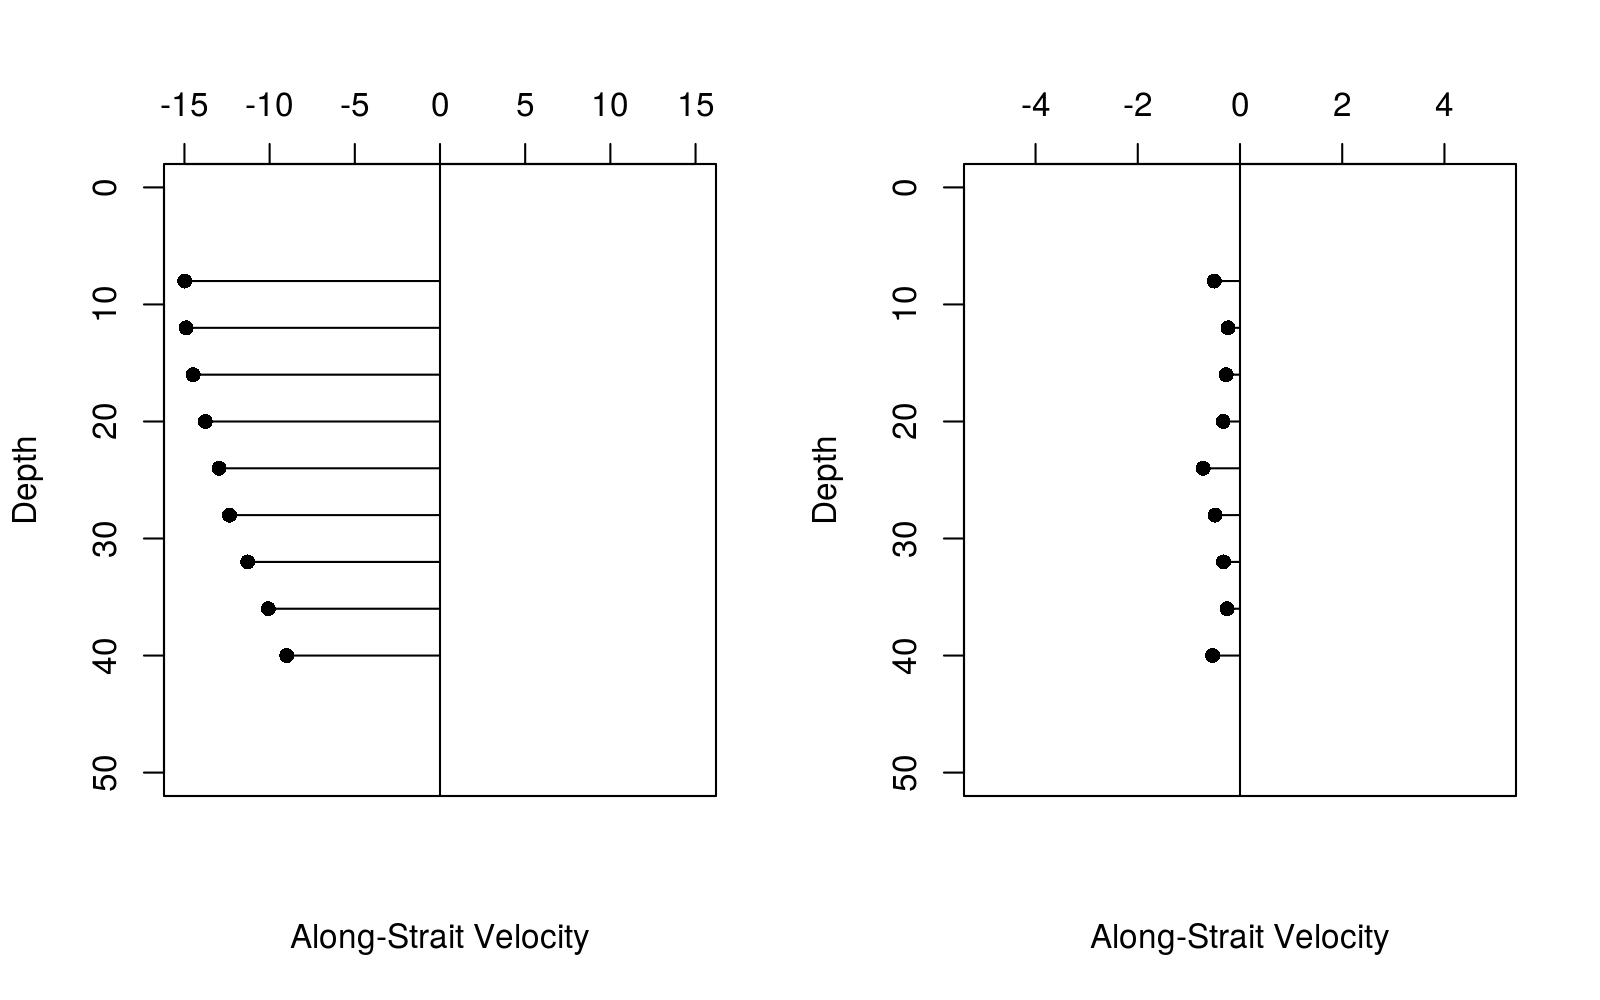
\includegraphics[width = 0.8\textwidth]{./figures/39_smf_lateSummer_2015.png}
\caption[Mean flow, Late Summer, 2015]{Mean flow, Late Summer: August 2015 to September 2015}
\label{f:smf_ls_2015}
\end{figure}


\begin{figure}  
\centering
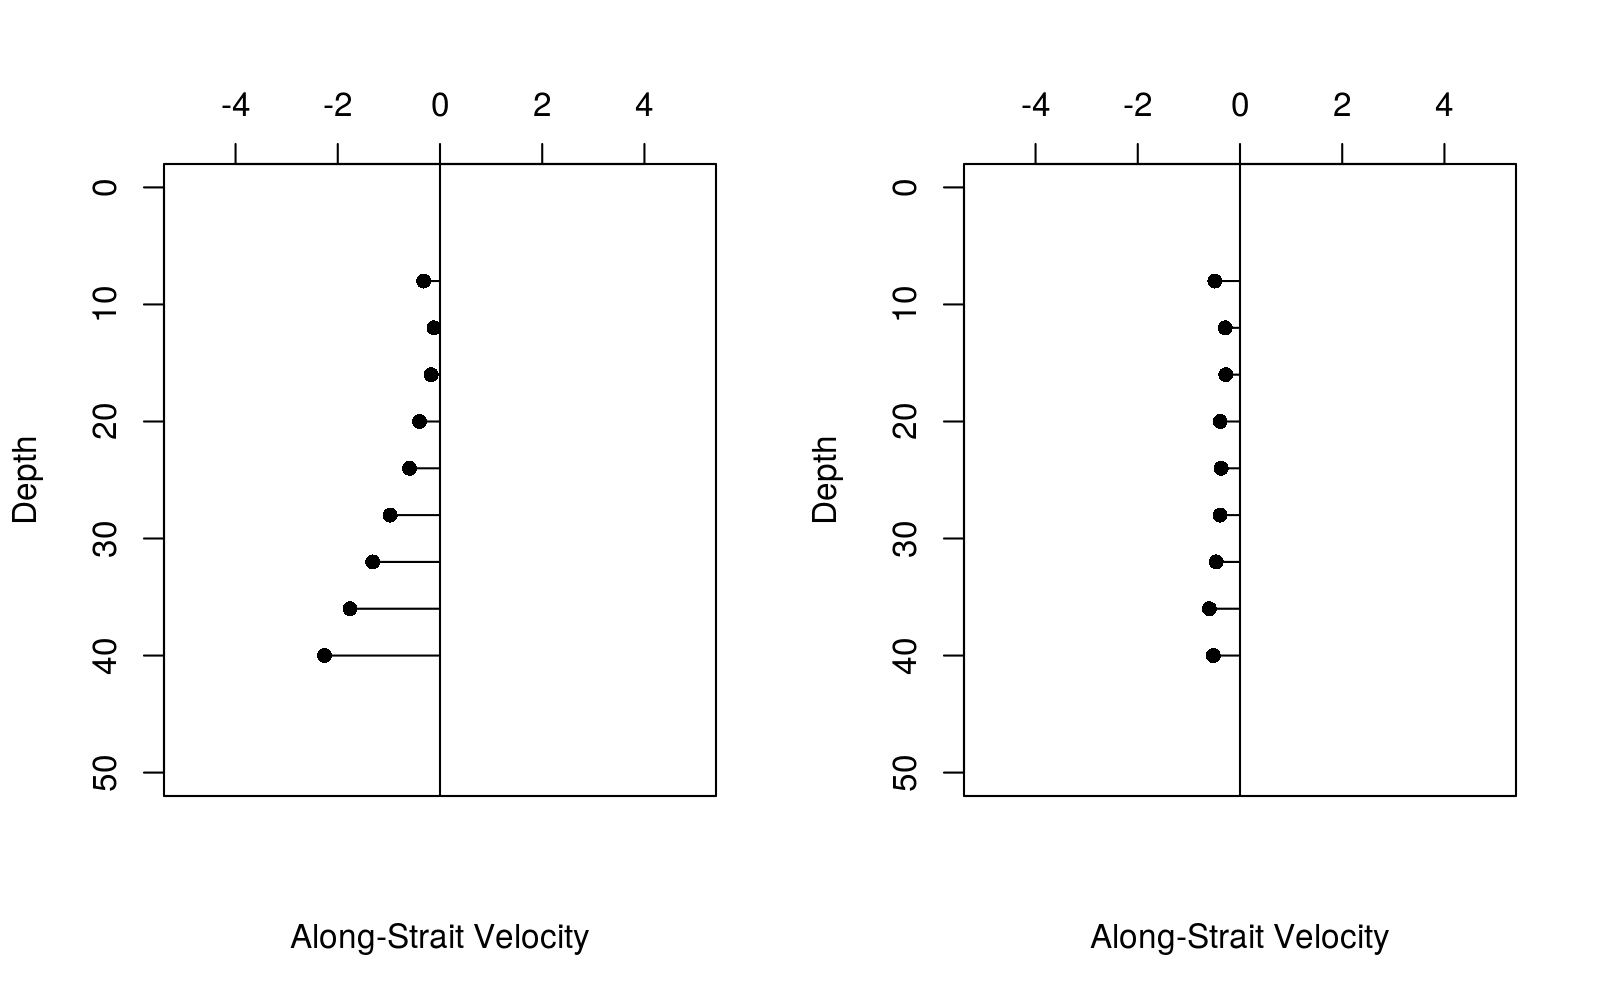
\includegraphics[width = 0.8\textwidth]{./figures/40_smf_fall_2014.png}
\caption[Mean flow, Fall, 2014]{Mean flow, Fall: October 2014 - December 2014}
\label{f:smf_f_2014}
\end{figure}

\begin{figure}  
\centering
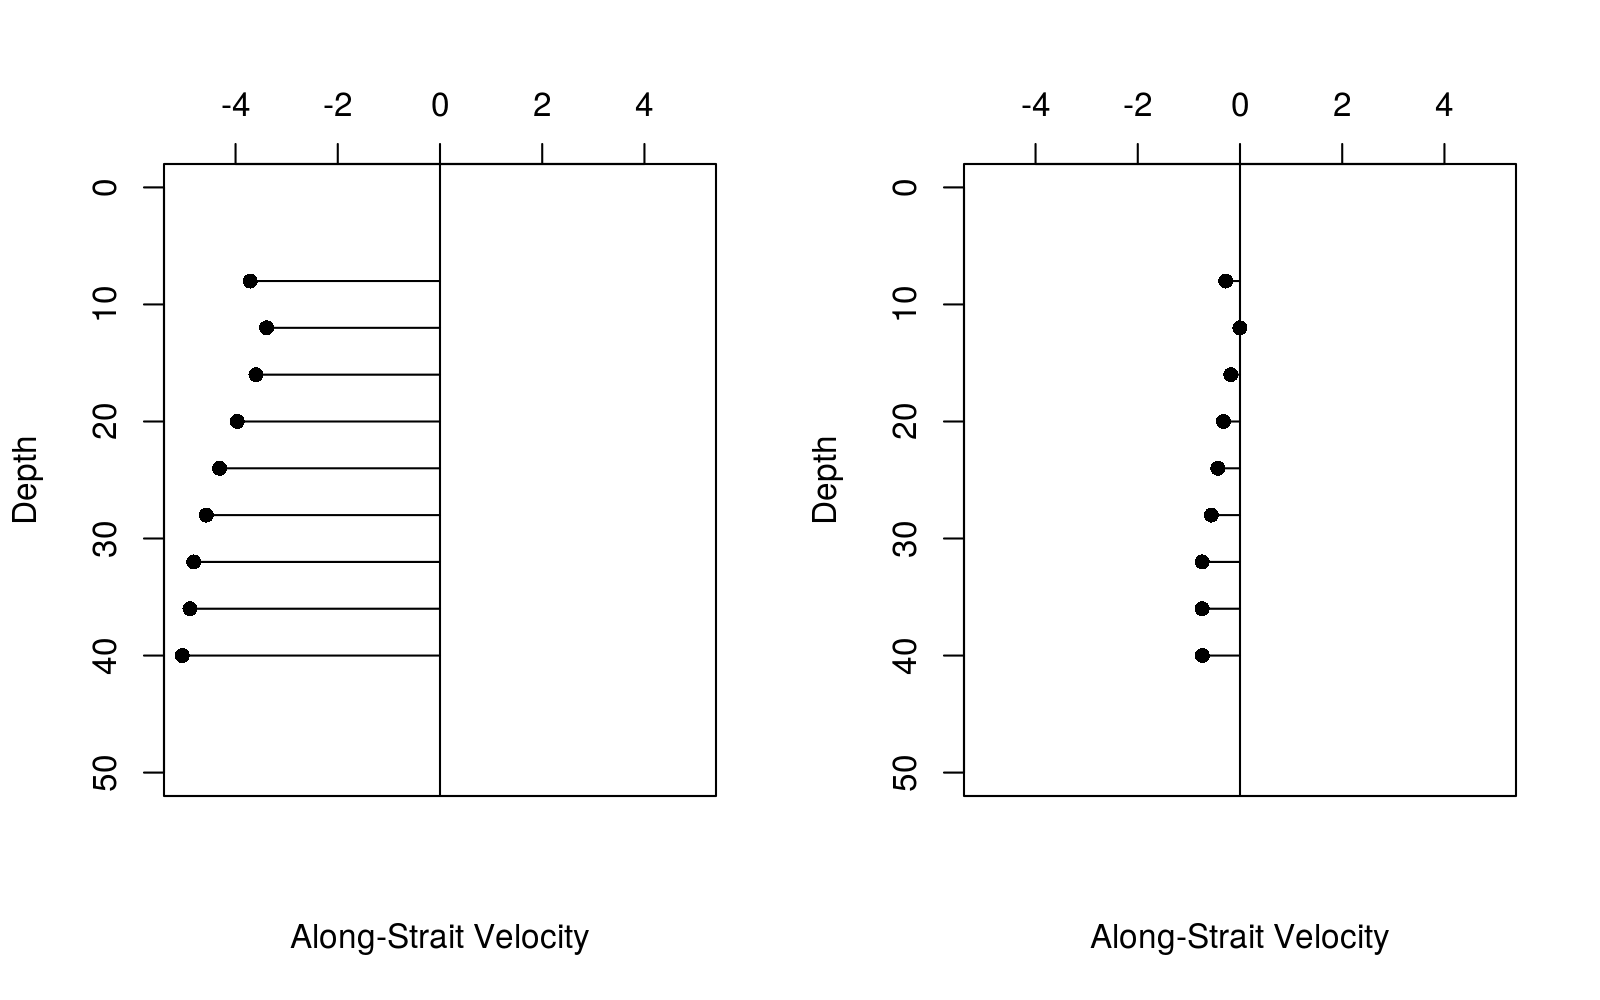
\includegraphics[width = 0.8\textwidth]{./figures/41_smf_fall_2015.png}
\caption[Mean flow, Fall, 2015]{Mean flow, Fall: October 2015 - December 2015}
\label{f:smf_f_2015}
\end{figure}


\begin{figure}  
\centering
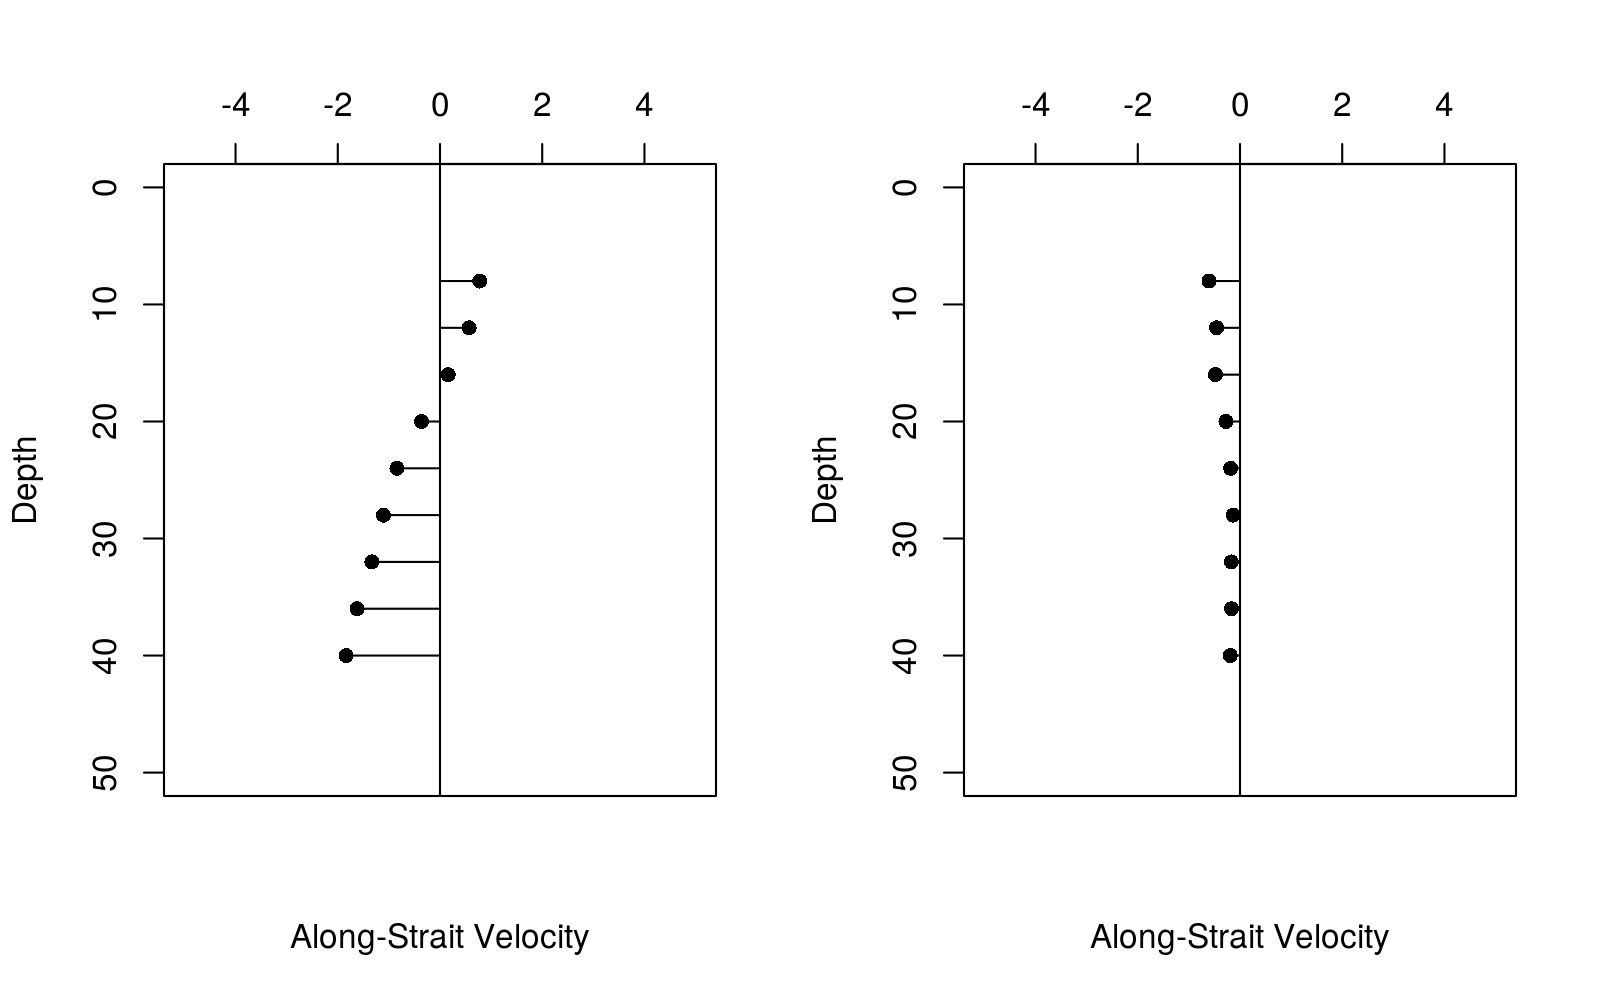
\includegraphics[width = 0.8\textwidth]{./figures/42_smf_winter_2015.png}
\caption[Mean flow, Winter, 2015]{Mean flow, Winter: January 2015 - March 2015}
\label{f:smf_w_2015}
\end{figure}

\begin{figure}  
\centering
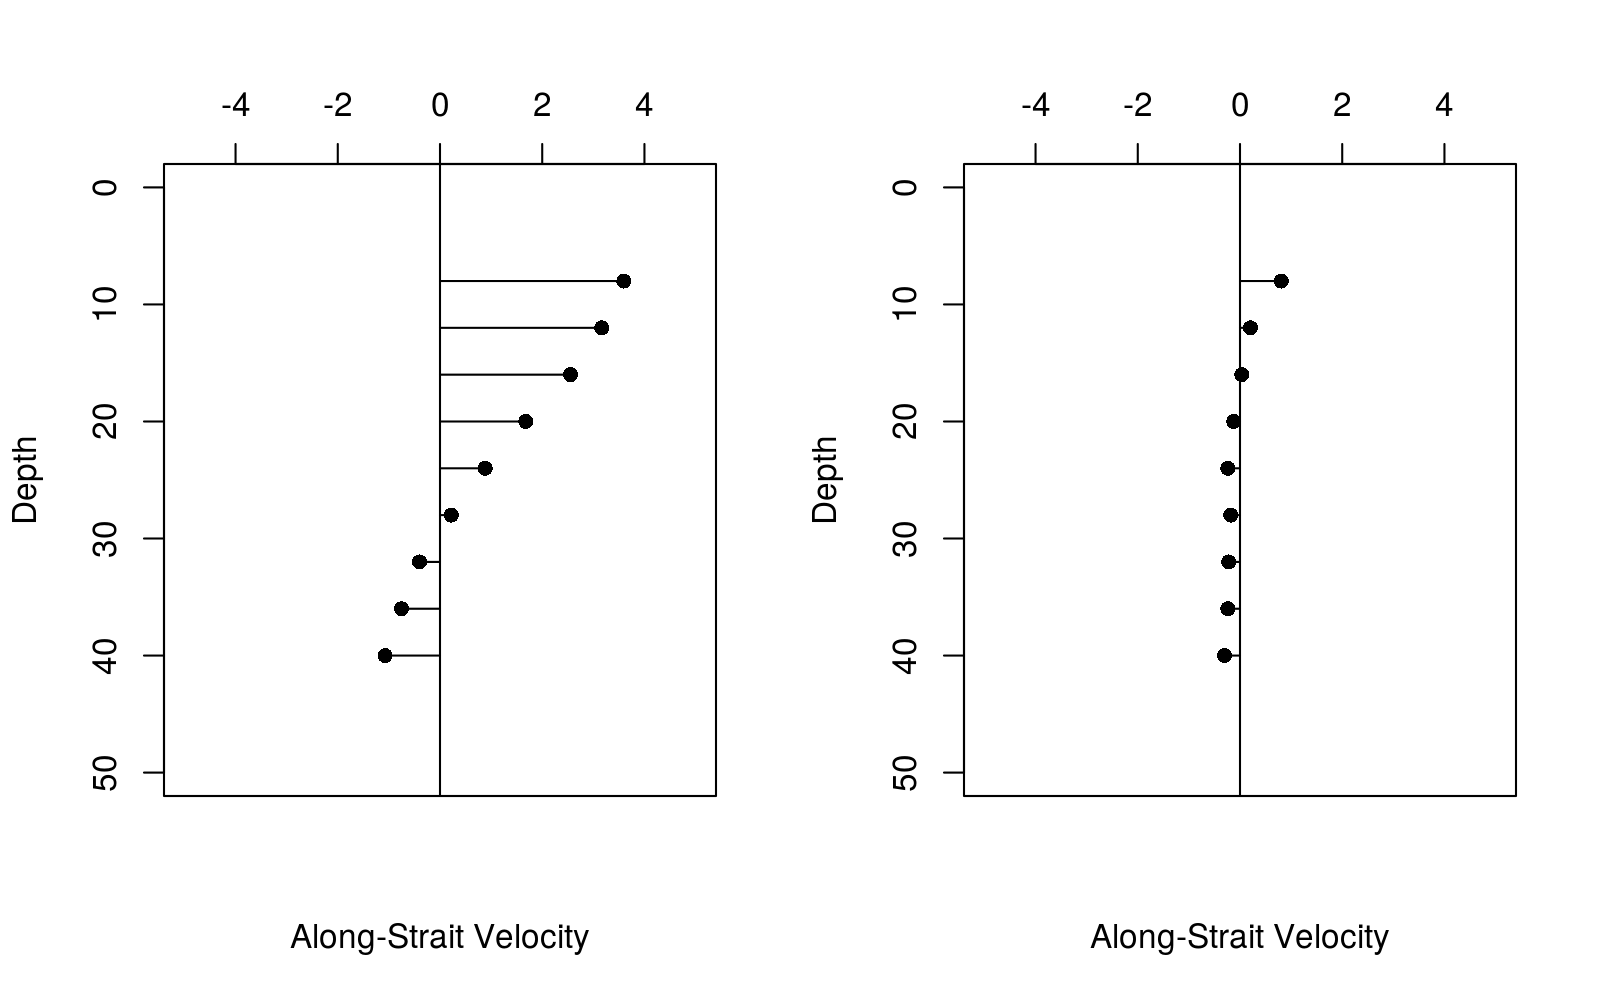
\includegraphics[width = 0.8\textwidth]{./figures/43_smf_winter_2016.png}
\caption[Mean flow, Winter, 2016]{Mean flow, Winter: January 2016 - March 2016}
\label{f:smf_w_2016}
\end{figure}


\begin{figure}  
\centering
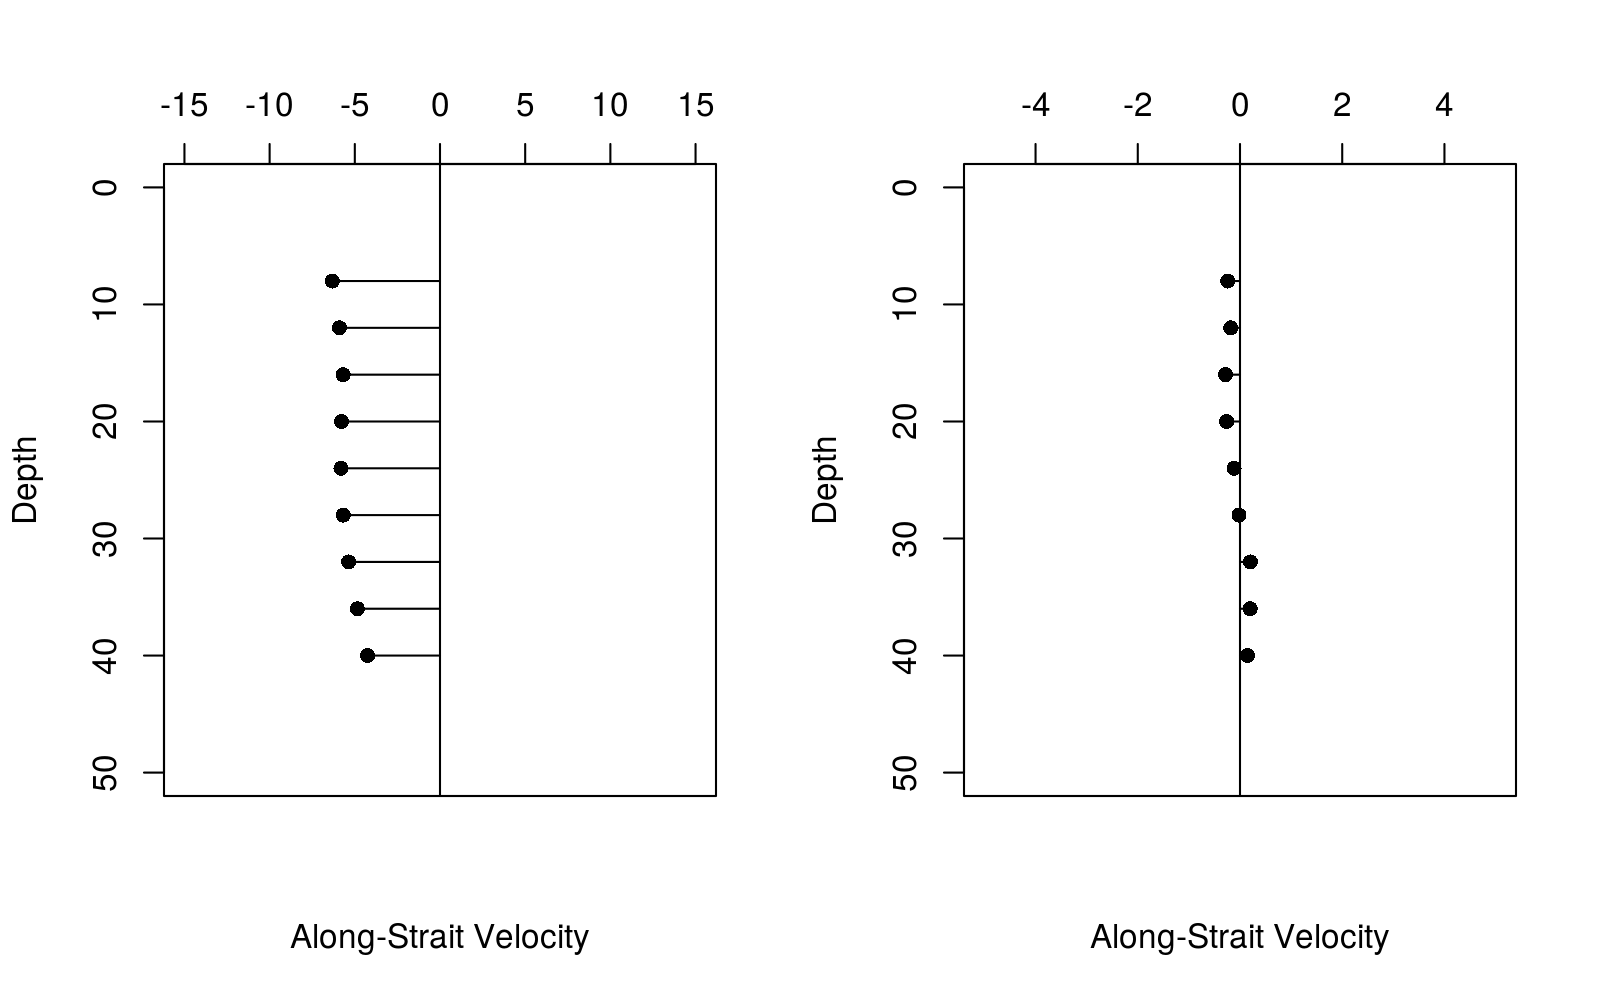
\includegraphics[width = 0.8\textwidth]{./figures/44_smf_spring_2015.png}
\caption[Mean flow, Spring, 2015]{Mean flow, Spring: April 2015 - June 2015}
\label{f:smf_s_2015}
\end{figure}

\begin{figure}  
\centering
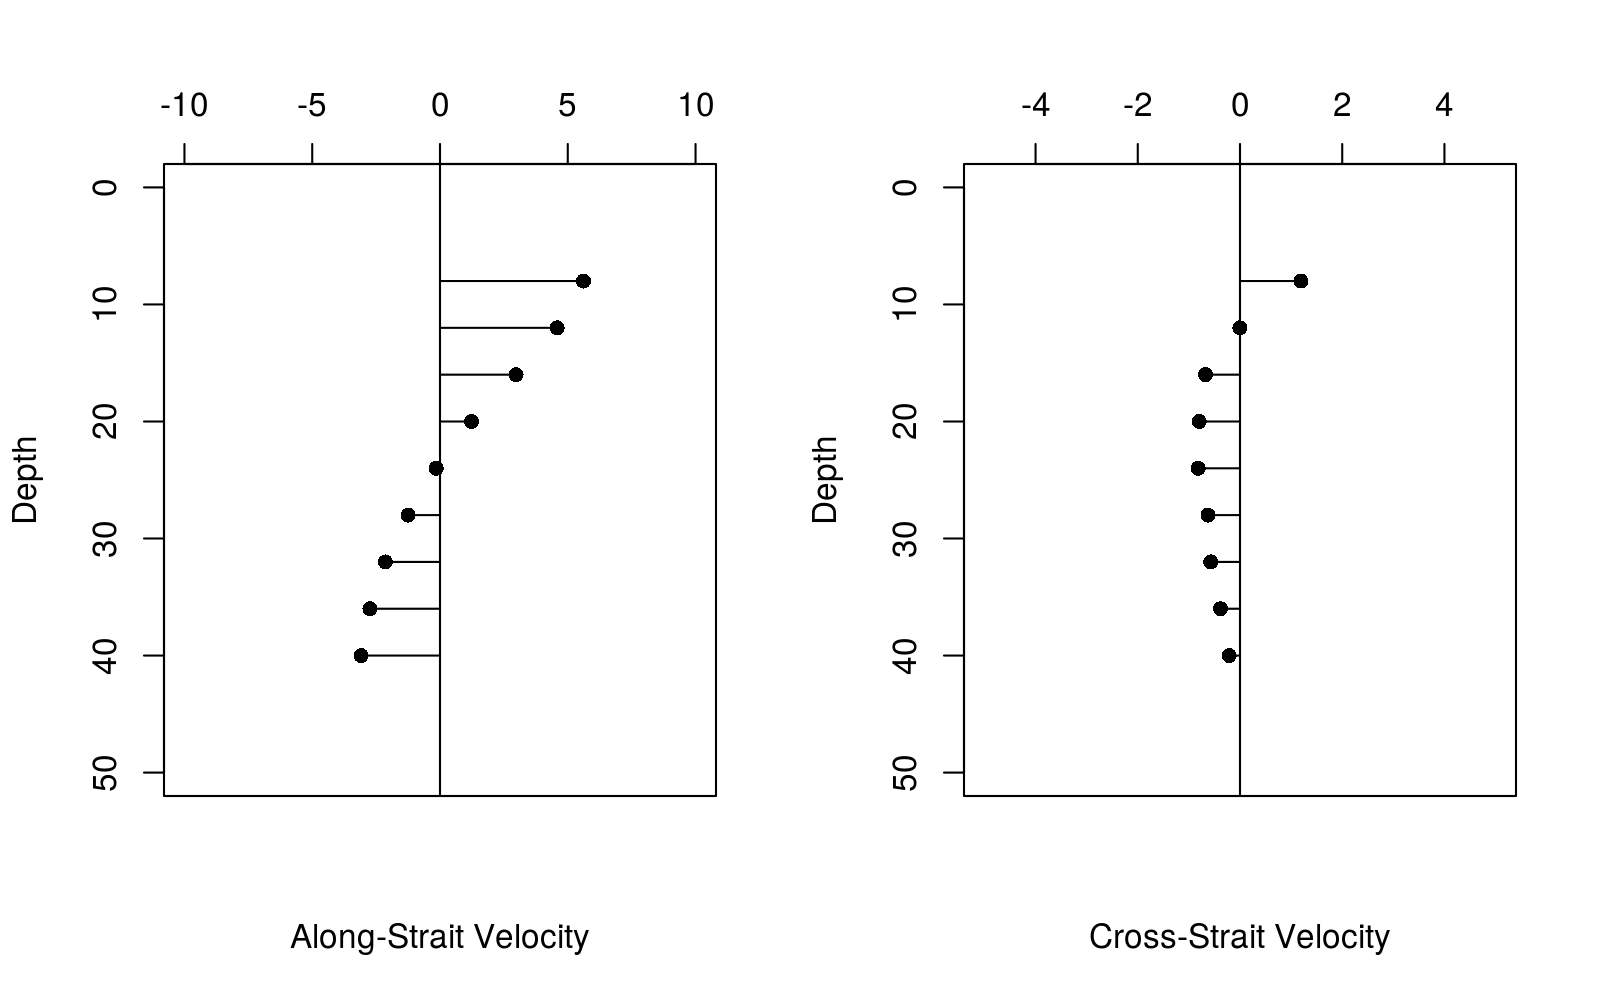
\includegraphics[width = 0.8\textwidth]{./figures/45_smf_spring_2016.png}
\caption[Mean flow, Spring, 2016]{Mean flow, Spring: April 2016 - June 2016}
\label{f:smf_s_2016}
\end{figure}


\begin{figure}  
\centering
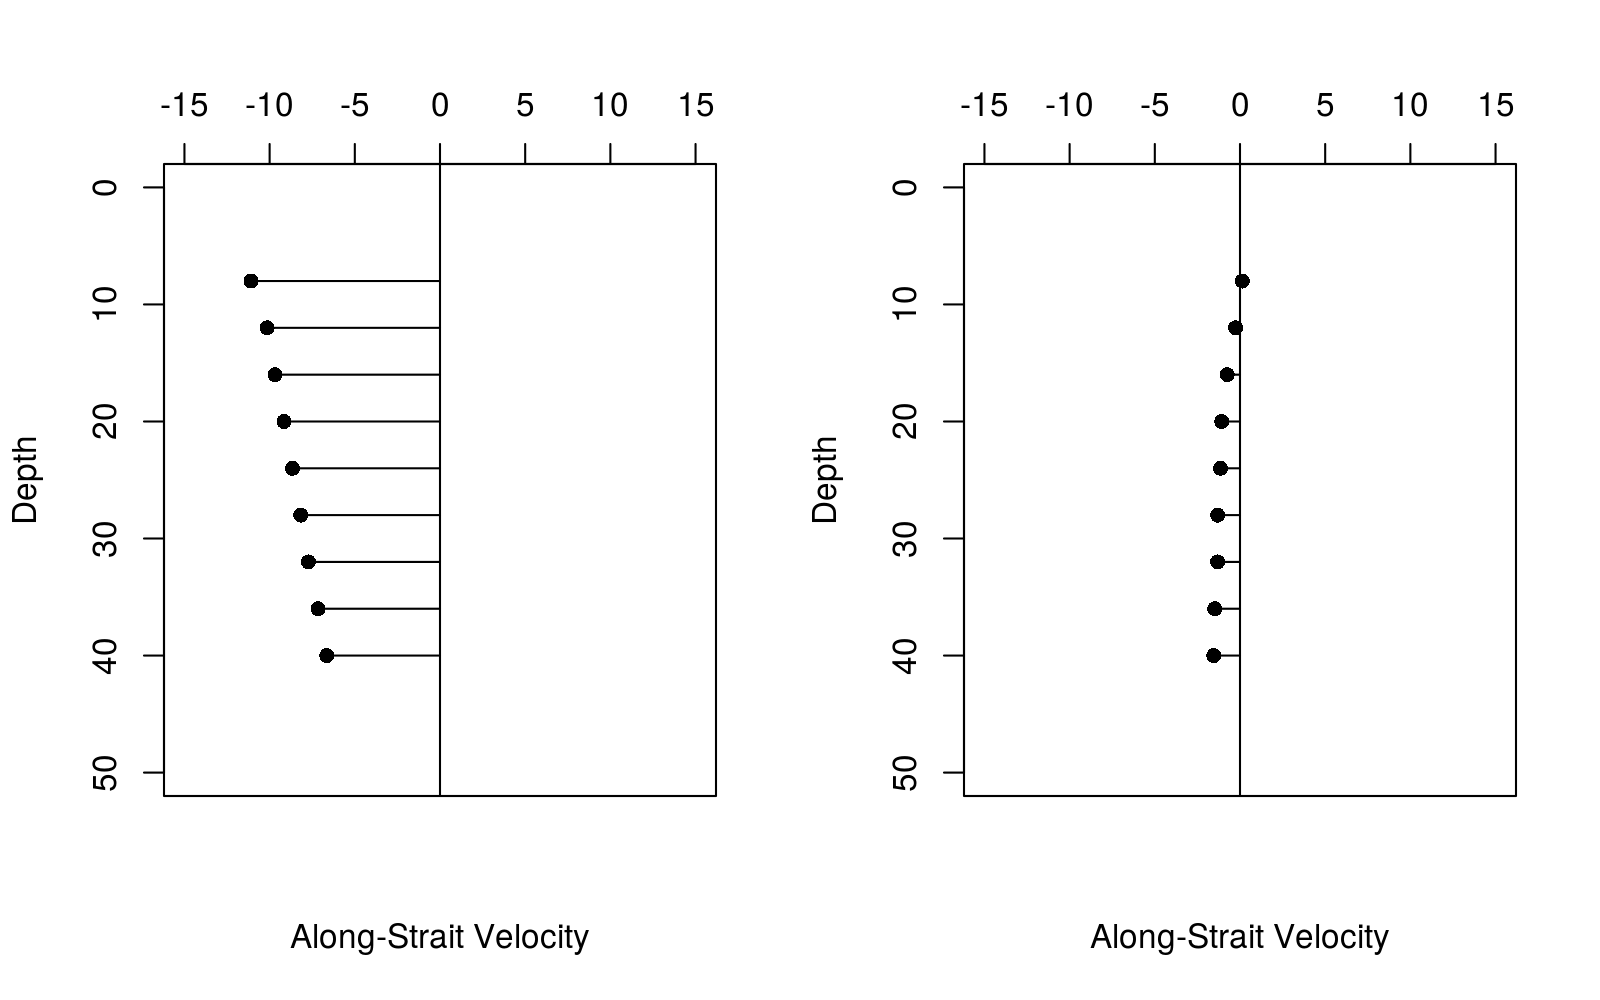
\includegraphics[width = 0.8\textwidth]{./figures/46_smf_earlySummer_2015.png}
\caption[Mean flow, Early Summer, 2015]{Mean flow, Early Summer: July 2015 - August 2015}
\label{f:smf_es_2015}
\end{figure}

\begin{figure}  
\centering
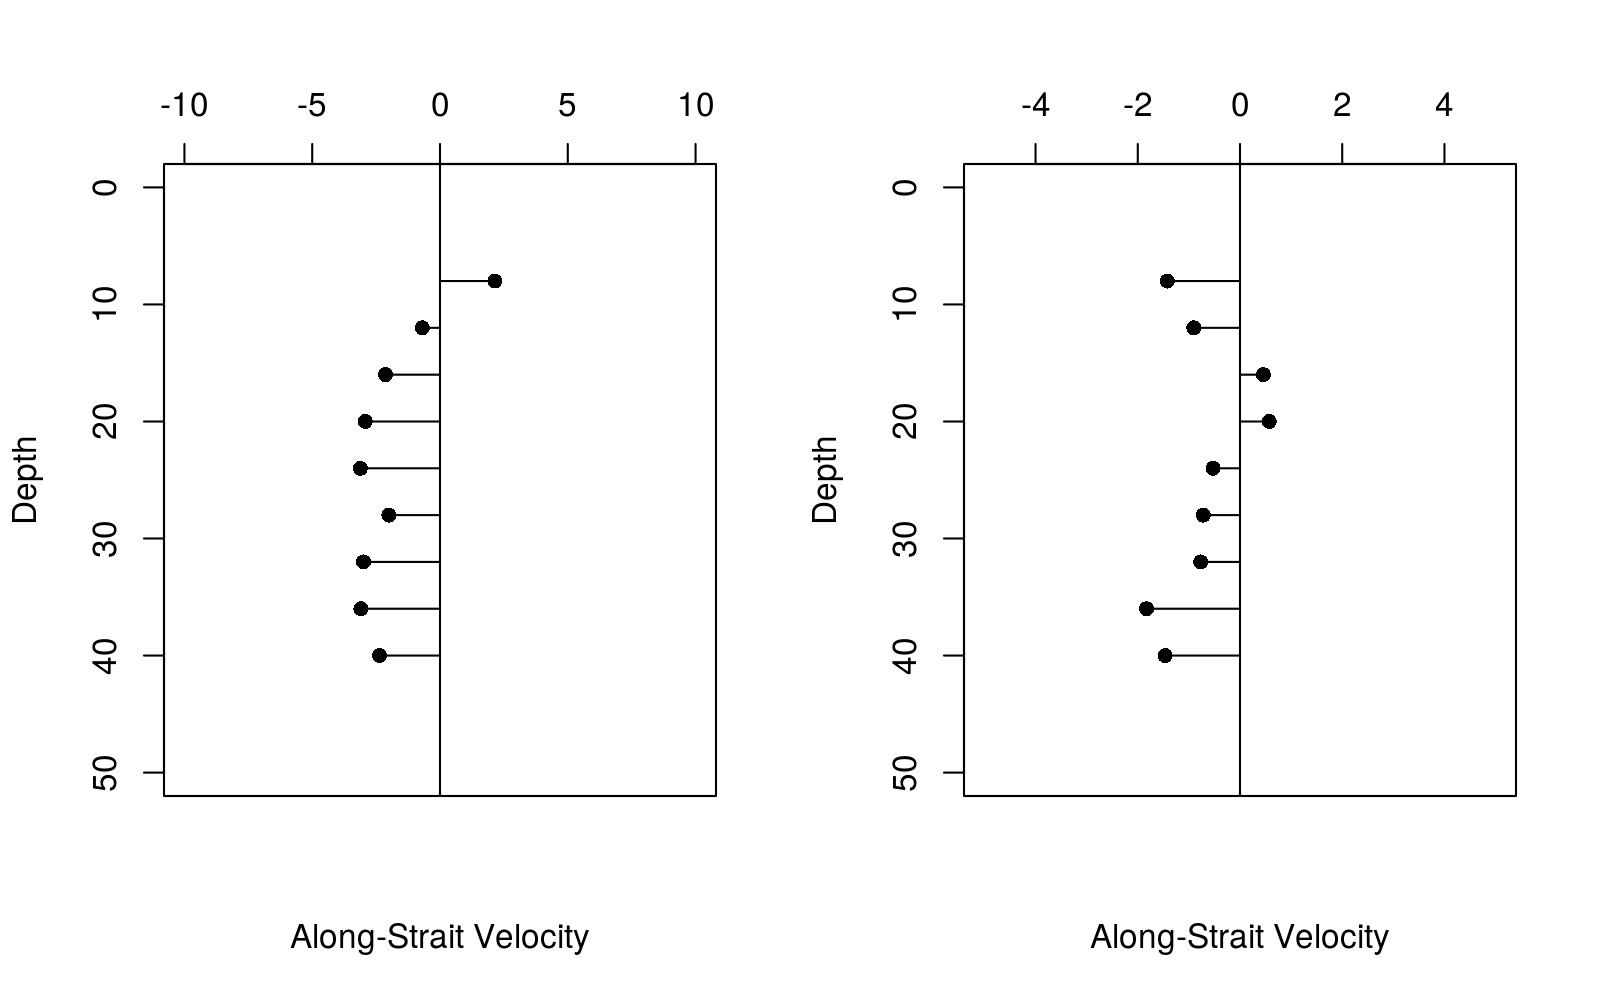
\includegraphics[width = 0.8\textwidth]{./figures/47_smf_earlySummer_2016.png}
\caption[Mean flow, Early Summer, 2016]{Mean flow, Early Summer: July 2016 - August 2016}
\label{f:smf_es_2016}
\end{figure}



\begin{figure}  
\centering
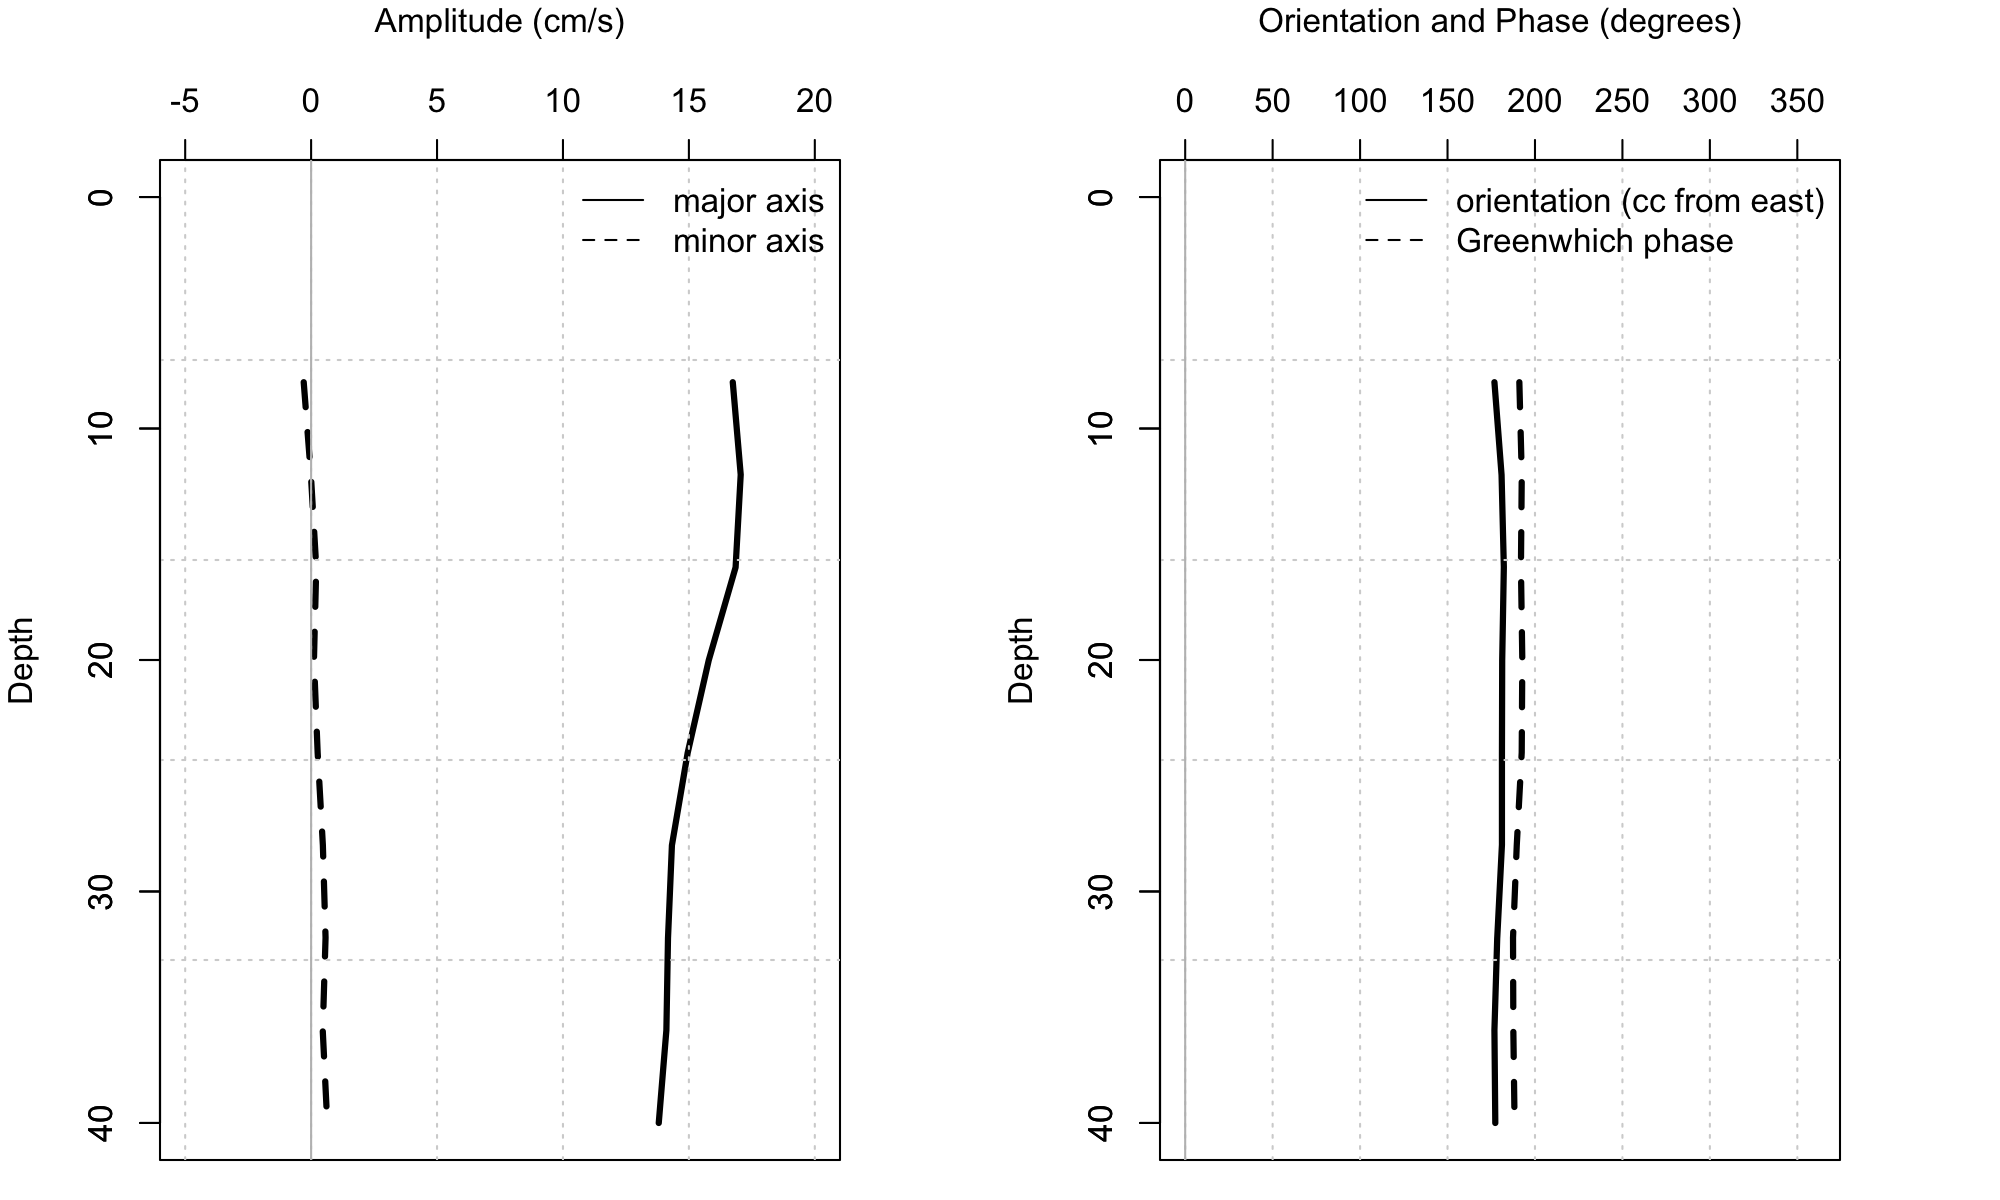
\includegraphics[width = 0.8\textwidth]{./figures/48_M2TC_if_2014.png}
\caption[M2 Tidal Constituents, Ice free, 2014]{M2 Tidal Constituents, Ice Free Period (August 12 2014 - September 27 2014)}
\label{f:m2_if_2014}
\end{figure}

\begin{figure}  
\centering
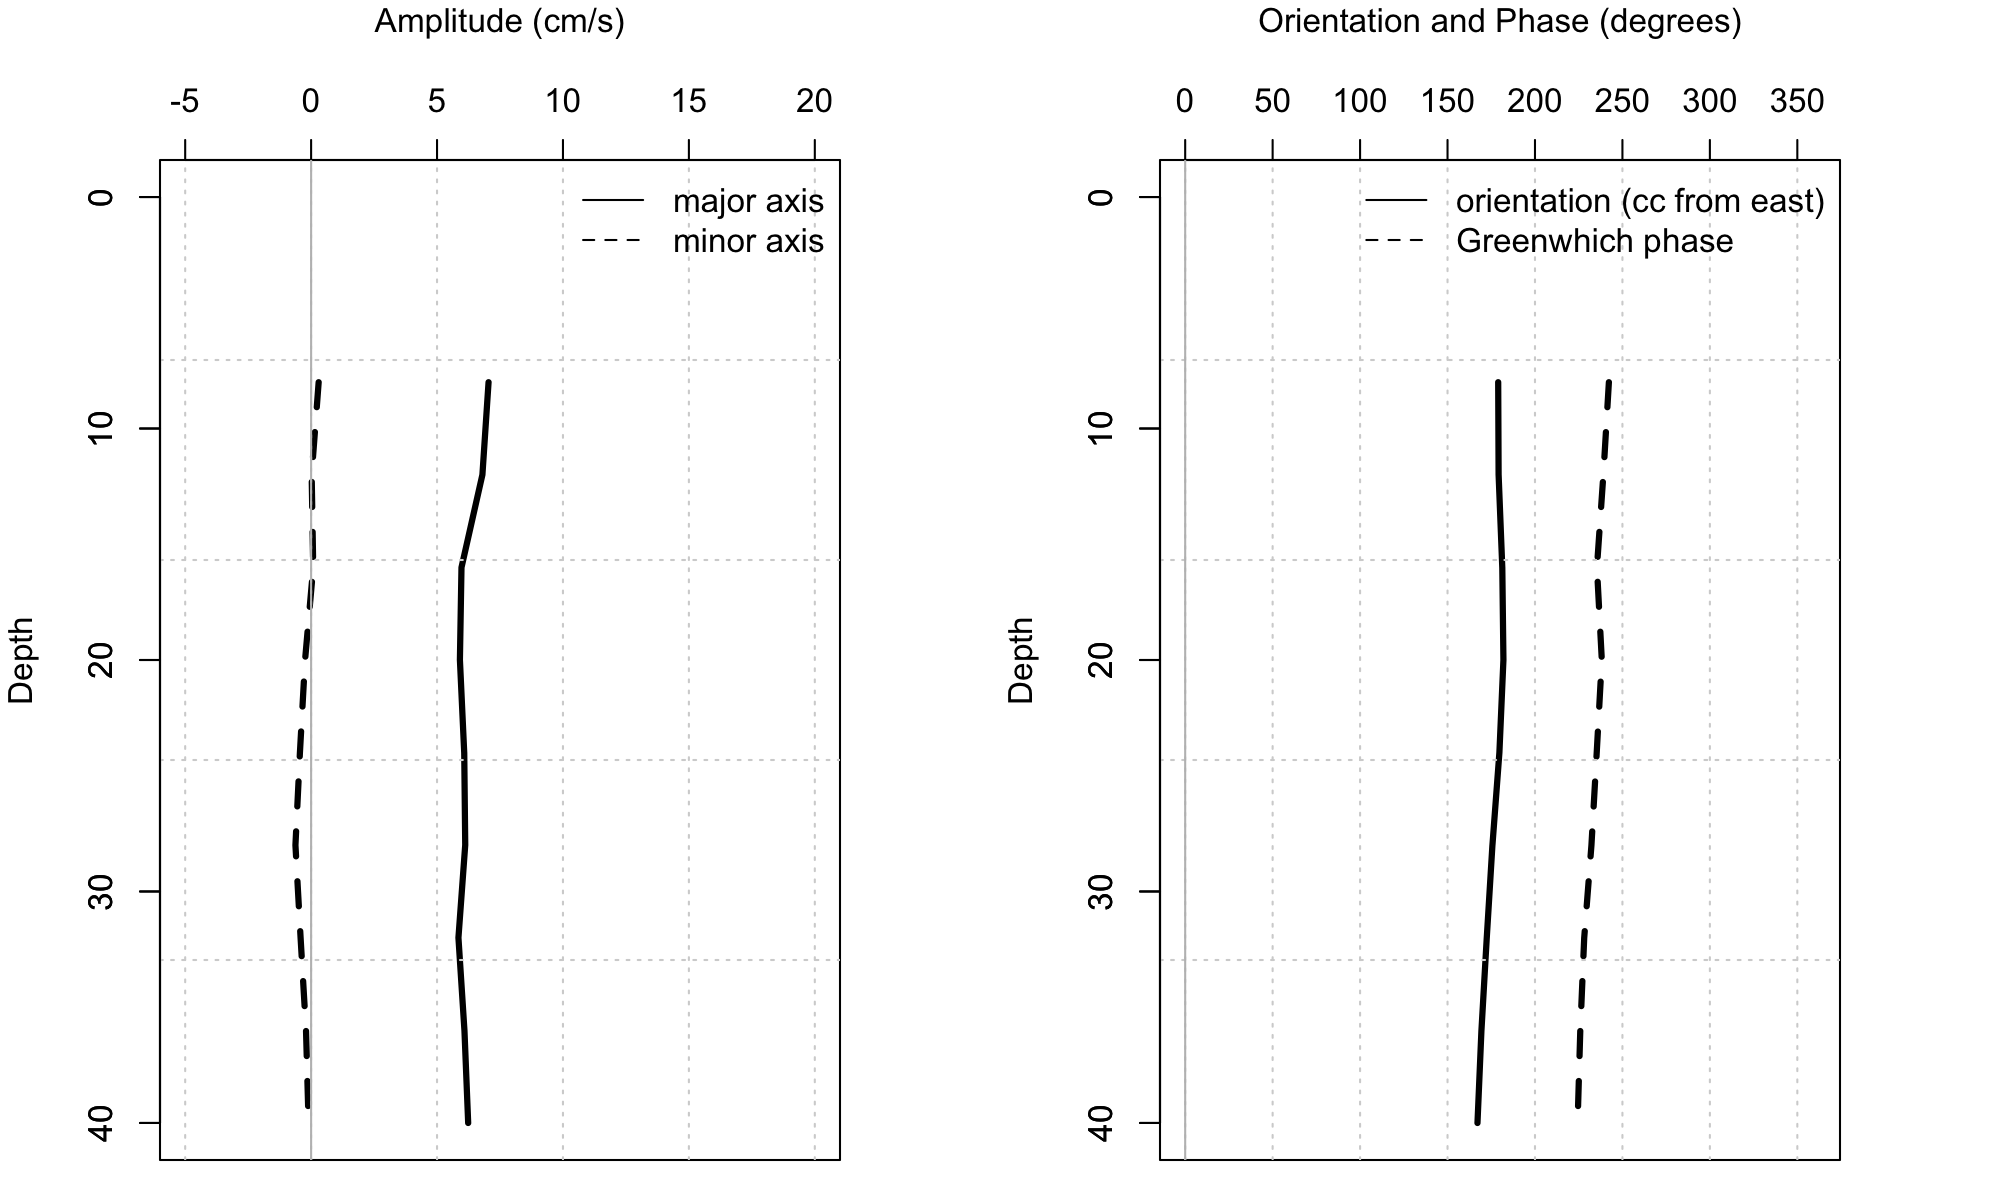
\includegraphics[width = 0.8\textwidth]{./figures/49_S2TC_if_2014.png}
\caption[S2 Tidal Constituents, Ice free, 2014]{S2 Tidal Constituents, Ice Free Period (August 12 2014 - September 27 2014)}
\label{f:s2_if_2014}
\end{figure}

\begin{figure}  
\centering
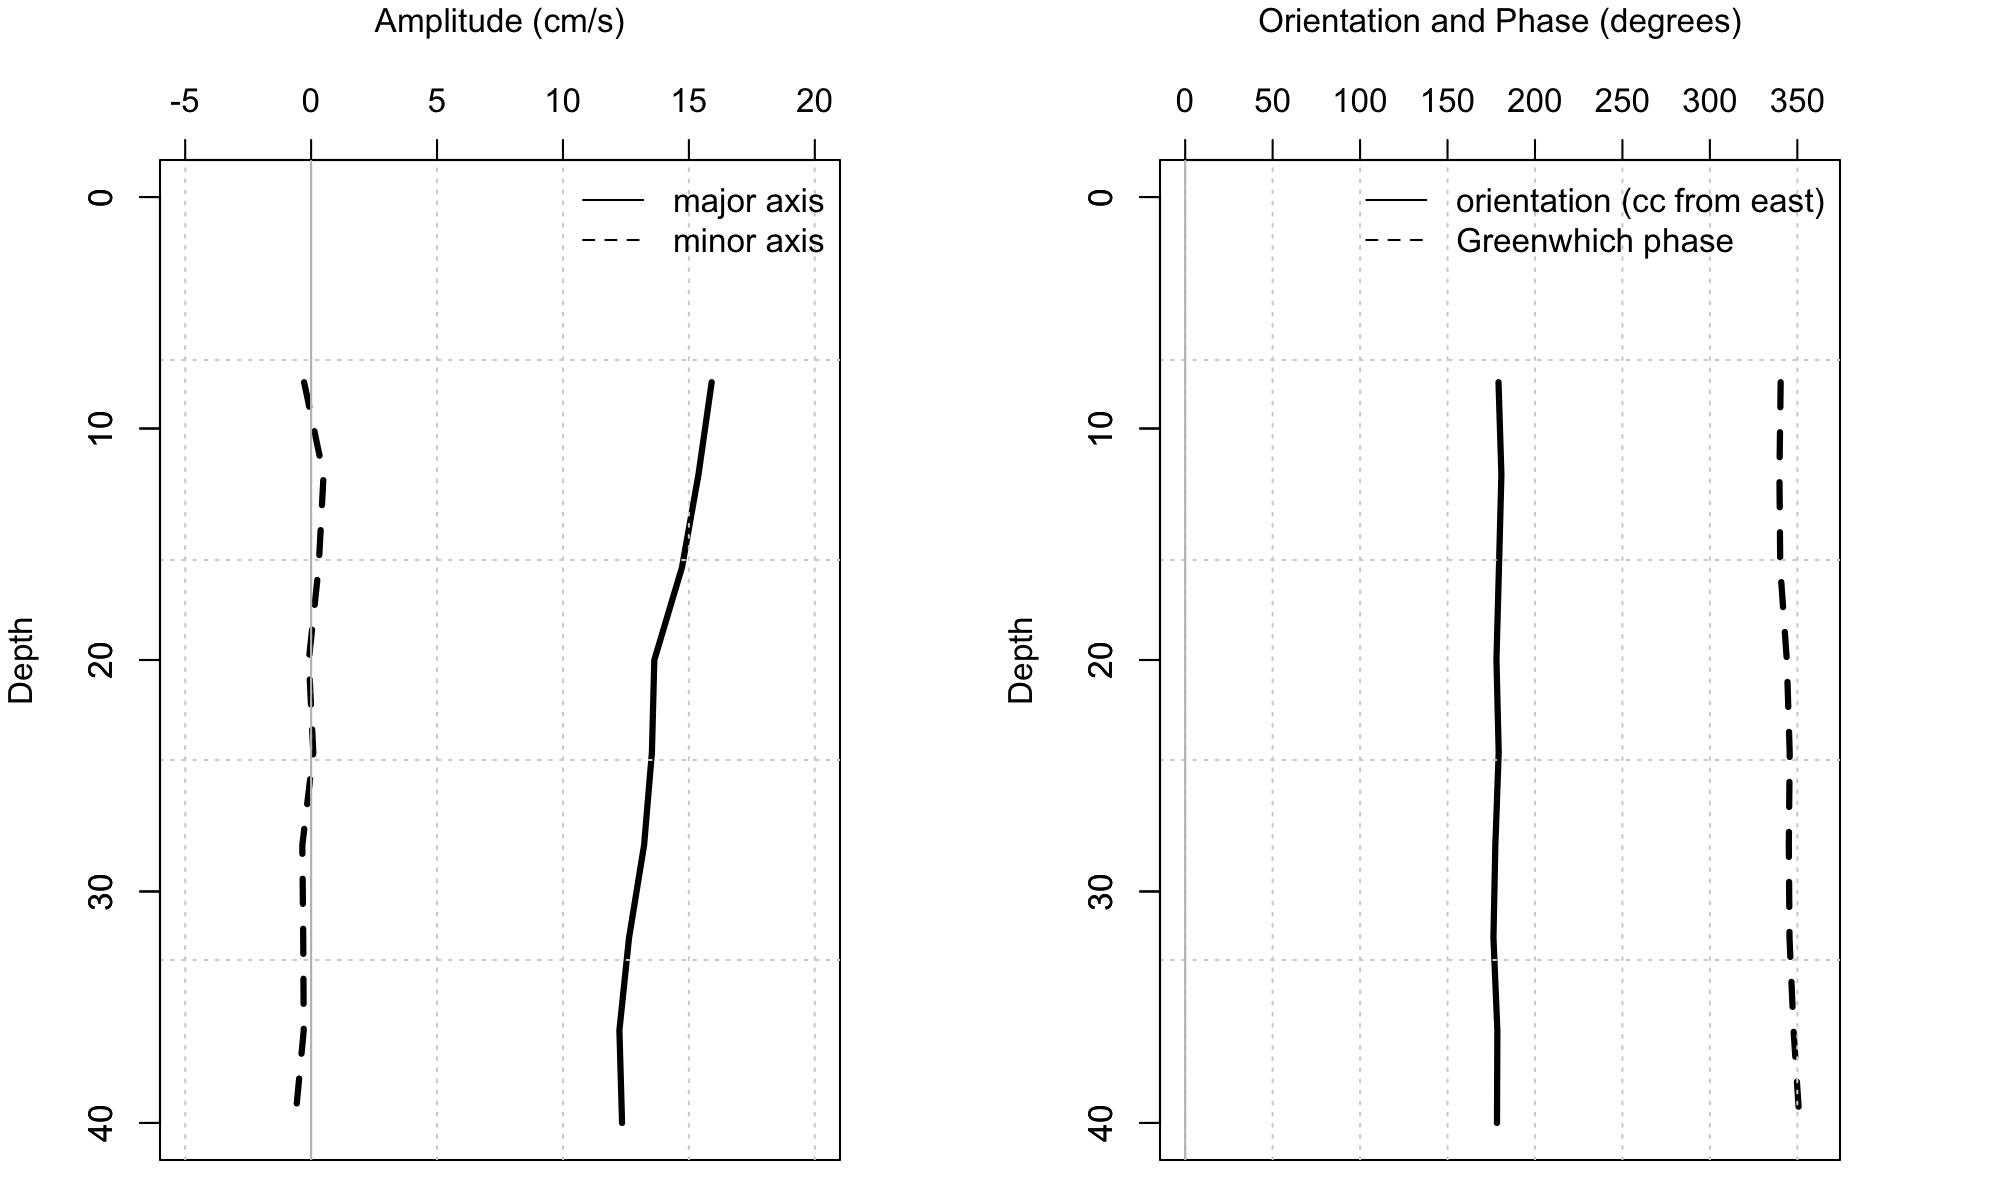
\includegraphics[width = 0.8\textwidth]{./figures/50_K1TC_if_2014.png}
\caption[K1 Tidal Constituents, Ice free, 2014]{K1 Tidal Constituents, Ice Free Period (August 12 2014 - September 27 2014)}
\label{f:k1_if_2014}
\end{figure}

\begin{figure}  
\centering
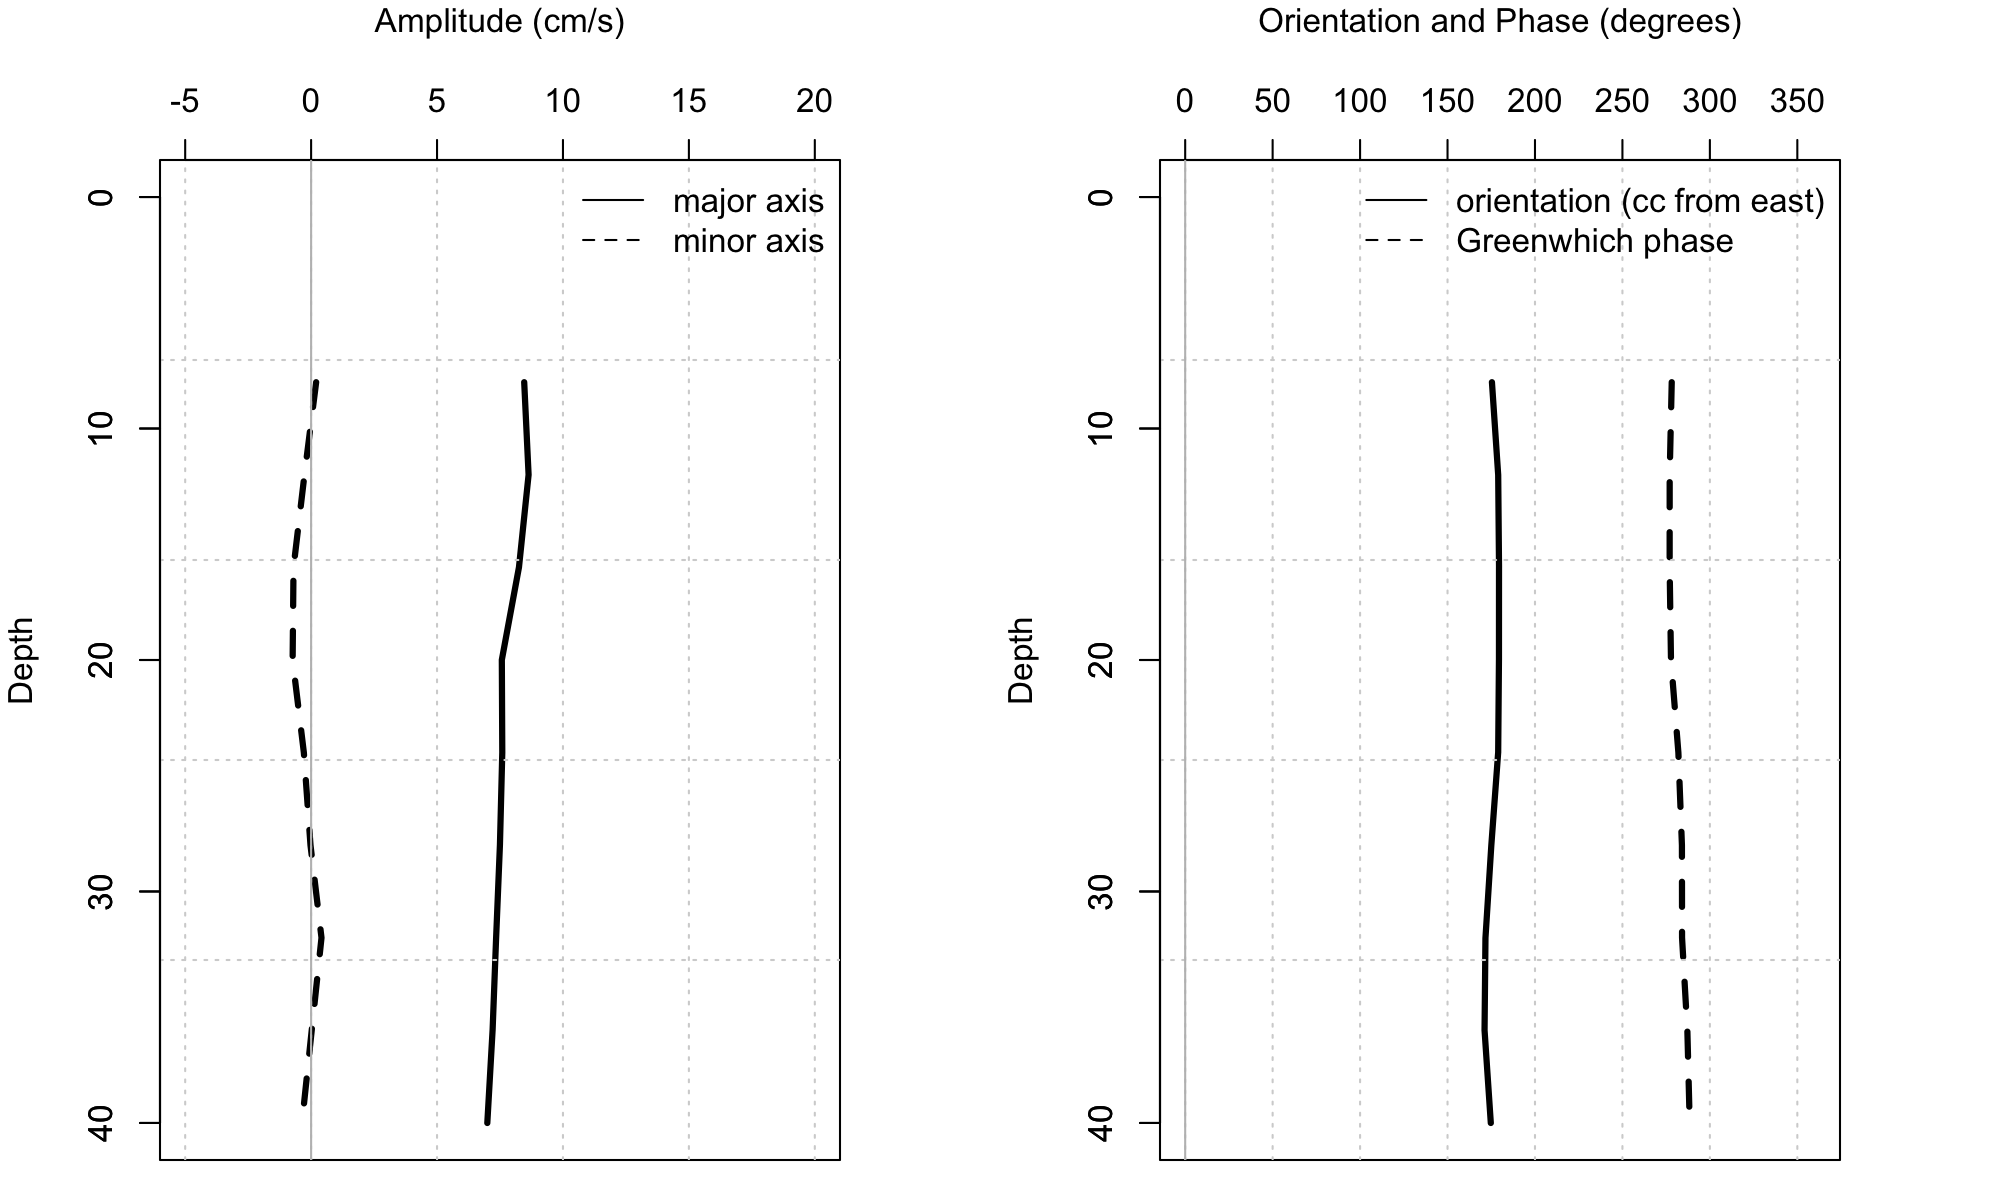
\includegraphics[width = 0.8\textwidth]{./figures/51_O1TC_if_2014.png}
\caption[O1 Tidal Constituents, Ice free, 2014]{O1 Tidal Constituents, Ice Free Period (August 12 2014 - September 27 2014)}
\label{f:o1_if_2014}
\end{figure}

\begin{figure}  
\centering
\includegraphics[width = 0.8\textwidth]{./figures/52_P1TC_if_2014.png}
\caption[P1 Tidal Constituents, Ice free, 2014]{P1 Tidal Constituents, Ice Free Period (August 12 2014 - September 27 2014)}
\label{f:p1_if_2014}
\end{figure}


\begin{figure}  
\centering
\includegraphics[width = 0.8\textwidth]{./figures/53_M2TC_if_2015.png}
\caption[M2 Tidal Constituents, Ice free, 2015]{M2 Tidal Constituents, Ice Free Period (July 15 2015 - September 27 2015)}
\label{f:m2_if_2015}
\end{figure}

\begin{figure}  
\centering
\includegraphics[width = 0.8\textwidth]{./figures/54_M2TC_si_2015.png}
\caption[M2 Tidal Constituents, Solid Ice, 2015]{M2 Tidal Constituents, Solid Ice Period (March 1 2016 - July 1 2016)}
\label{f:m2_si_2015}
\end{figure}


\begin{figure}  
\centering
\includegraphics[width = 0.8\textwidth]{./figures/55_S2TC_if_2015.png}
\caption[S2 Tidal Constituents, Ice free, 2015]{S2 Tidal Constituents, Ice Free Period (July 15 2015 - September 27 2015)}
\label{f:s2_if_2015}
\end{figure}

\begin{figure}  
\centering
\includegraphics[width = 0.8\textwidth]{./figures/56_S2TC_si_2015.png}
\caption[S2 Tidal Constituents, Solid Ice, 2015]{S2 Tidal Constituents, Solid Ice Period (March 1 2016 - July 1 2016)}
\label{f:s2_si_2015}
\end{figure}


\begin{figure}  
\centering
\includegraphics[width = 0.8\textwidth]{./figures/57_K1TC_if_2015.png}
\caption[K1 Tidal Constituents, Ice free, 2015]{K1 Tidal Constituents, Ice Free Period (July 15 2015 - September 27 2015)}
\label{f:k1_if_2015}
\end{figure}

\begin{figure}  
\centering
\includegraphics[width = 0.8\textwidth]{./figures/58_K1TC_si_2015.png}
\caption[K1 Tidal Constituents, Solid Ice, 2015]{K1 Tidal Constituents, Solid Ice Period (March 1 2016 - July 1 2016)}
\label{f:k1_si_2015}
\end{figure}


\begin{figure}  
\centering
\includegraphics[width = 0.8\textwidth]{./figures/59_O1TC_if_2015.png}
\caption[O1 Tidal Constituents, Ice free, 2015]{O1 Tidal Constituents, Ice Free Period (July 15 2015 - September 27 2015)}
\label{f:o1_if_2015}
\end{figure}

\begin{figure}  
\centering
\includegraphics[width = 0.8\textwidth]{./figures/60_O1TC_si_2015.png}
\caption[O1 Tidal Constituents, Solid Ice, 2015]{O1 Tidal Constituents, Solid Ice Period (March 1 2016 - July 1 2016)}
\label{f:o1_si_2015}
\end{figure}


\begin{figure}  
\centering
\includegraphics[width = 0.8\textwidth]{./figures/61_P1TC_if_2015.png}
\caption[P1 Tidal Constituents, Ice free, 2015]{P1 Tidal Constituents, Ice Free Period (July 15 2015 - September 27 2015)}
\label{f:p1_if_2015}
\end{figure}

\begin{figure}  
\centering
\includegraphics[width = 0.8\textwidth]{./figures/62_P1TC_si_2015.png}
\caption[P1 Tidal Constituents, Solid Ice, 2015]{P1 Tidal Constituents, Solid Ice Period (March 1 2016 - June 1 2016)}
\label{f:p1_si_2015}
\end{figure}



\begin{figure}  
\centering
\includegraphics[width = 0.8\textwidth]{./figures/63_iceDraft_2014_2015.png}
\caption[Ice Draft, 2014-2015]{Ice Draft: monthly time series, August 2014 - July 2015}
\label{f:id_2014_2015}
\end{figure}

\begin{figure}  
\centering
\includegraphics[width = 0.8\textwidth]{./figures/64_iceDraft_2015_2016.png}
\caption[Ice Draft, 2015-2016]{Ice Draft: monthly time series, August 2015 - July 2016}
\label{f:id_2015_2016}
\end{figure}




\begin{figure}  
\centering
\includegraphics[width = 0.8\textwidth]{./figures/65_iceHist_2014_2015.png}
\caption[Histograms of ice draft, 2014-2015]{Monthly Histograms of Ice Draft, August 2014 - August 2015}
\label{f:ih_2014_2015}
\end{figure}

\begin{figure}  
\centering
\includegraphics[width = 0.8\textwidth]{./figures/66_iceHist_2015_2016.png}
\caption[Histograms of ice draft, 2015-2016]{Monthly Histograms of Ice Draft, August 2015 - August 2016}
\label{f:ih_2015_2016}
\end{figure}



\begin{figure}  
\centering
\includegraphics[width = 0.8\textwidth]{./figures/67_iceDraftStat_2014_2015.png}
\caption[Ice draft Statistics, 2014-2015]{Ice Draft Statistics from Ice Profiling Sonar, August 2014 - July 2015}
\label{f:ids_2014_2015}
\end{figure}

\begin{figure}  
\centering
\includegraphics[width = 0.8\textwidth]{./figures/68_iceDraftStat_2015_2016.png}
\caption[Ice draft Statistics, 2015-2016]{Ice Draft Statistics from Ice Profiling Sonar, August 2015 - July 2016}
\label{f:ids_2015_2016}
\end{figure}
  


\begin{figure}  
\centering
\includegraphics[width = 0.8\textwidth]{./figures/69_iceVel_2014_2015.png}
\caption[Ice Velocity, 2014-2015]{Ice Velocity, August 2014 - August 2015}
\label{f:ivel_2014_2015}
\end{figure}

\begin{figure}  
\centering
\includegraphics[width = 0.8\textwidth]{./figures/70_iceVel_2015_2016.png}
\caption[Ice Velocity, 2015-2016]{Ice Velocity, August 2015 - August 2016}
\label{f:ivel_2015_2016}
\end{figure}



% latex table generated in R 3.6.1 by xtable 1.8-4 package
\begin{landscape}

\begin{table}[ht]
\centering
\caption[Mooring and Instrument Summary, 2011-2016]{Mooring and Instrument Summary, 2011-2016.} 
\label{t:mooringSummary}
\begin{tabular}{p{0.3in}p{.7in}p{.7in}p{.7in}p{.7in}p{.7in}p{.7in}p{.7in}p{.7in}p{.7in}p{.7in}p{.7in}}
 Year & BIO Consecutive Mooring Number & Mooring Name & Instrument Type & Serial Number & Moored Depth (m) & Sounding (m) & Latitude ($^\circ$ N) & Longitude ($^\circ$ W) & Start Date-Time (UTC) & End Date-Time (UTC) & Sampling Interval (Seconds) \\ 
  \hline
2011 & 1801 & Hub & CTD & 361 & 120 & 122 & 74.62443 & -91.29958 & 07-Aug-2011 00:00 & 07-Aug-2012 00:00 & 3600 \\ 
   \hline
\end{tabular}
\end{table}


\begin{table}[ht]
\centering
\caption[Microcat/ADCP statistical summary, 2011-2012]{Microcat/ADCP statistical summary, 2011-2016.} 
\label{t:ss_2011_2012}
\begin{tabular}{p{0.3in}p{0.3in}p{.2in}p{.2in}p{.2in}p{.2in}p{.2in}p{.2in}p{.2in}p{.2in}p{.2in}p{.2in}p{.2in}p{.2in}p{.2in}p{.2in}p{.2in}p{.2in}p{.2in}p{.2in}p{.2in}p{.2in}p{.2in}p{.2in}p{.2in}p{.2in}}

\multicolumn{2}{c}{Depth (m)} & \multicolumn{4}{c}{\textbf{Temperature ($^\circ$ C)}} & \multicolumn{4}{c}{\textbf{Salinity (psu)}} & \multicolumn{4}{c}{\textbf{Density (Sigma-T)}} & \multicolumn{4}{c}{\textbf{Along-Strait Velocity (cm/s)}} & \multicolumn{4}{c}{\textbf{Cross-Strait Velocity (cm/s)}}\\\hline
CTD & ADCP & Avg & SD & Min & Max & Avg & SD & Min & Max & Avg & SD & Min & Max & Avg & SD & Min & Max & Avg & SD & Min & Max \\ 
\hline
x & x & x & x & x & x & x & x & x & x & x & x & x & x & x & x & x & x & x & x & x & x 
\\ 
\hline  
\end{tabular}
\end{table}






\end{landscape}


\end{document}

